
\documentclass[10pt,openany]{ctexbook}
\usepackage{geometry}
%\usepackage{wallpaper}
\geometry{a4paper,left=3cm,right=2.2cm,top=3cm,bottom=2.5cm,headsep=16pt,headheight=2cm,}
%\usepackage[bookmarksopenlevel=2]{hyperref}
\usepackage{chemfig}
\usepackage{amsmath}
\begin{document}
\begin{titlepage}
\begin{center}
~~~~~~~~~~~~~~~~~~~~~~~~~~~~~~~~~~~~~\\
%\ThisCenterWallPaper{1}{666.pdf}
\vspace{6cm}\zihao{-0}{\heiti 洁~~净~~煤~~技~~术} \\ {\zihao{-0}PPT\zihao{-0}\heiti{排版} } \\ \vspace{3cm}
\zihao{3}刘~志~红~~~~~教~授
\thispagestyle{empty}
\end{center}
\end{titlepage}
\thispagestyle{empty}
\newpage
%~~~~~~~~~
%\newpage
\thispagestyle{empty}
~~\par
\vspace{1.5cm}
{\center \kaishu \zihao{3}声~~~明\par }
\vspace{0.6cm}

本排版为了期末考试,及平时学习所用,不作其他用途,本排版全部来源于刘志红教授PPT,在这里感谢感谢刘志红教授,还有感谢Zhuyong同学的封面设计,感谢http://bbs.ctex.org/论坛的技术支持。在这过程中用了半天时间,会有诸多错误,望日后在改。\par
\vspace{2.6cm}\hspace{10cm}——{\zihao{4}$Chen~yinghong$}\par
\vspace{0.2cm}\hspace{12.2cm}2014~年~5~月
\newpage
~
\thispagestyle{empty}
\newpage
\pagenumbering{arabic}
\tableofcontents

%\setcounter{page}{1}



\chapter{绪论}
\pagenumbering{arabic}
本章主要讲述洁净煤技术的概念;我国洁净煤技术重点发展的领域 ;国内外洁净煤技术发展状况及意义;清洁生产概念。
要求重点掌握洁净煤技术的概念及我国洁净煤技术重点发展的4个领域和10个方面;一般掌握国内洁净煤技术的发展状况、清洁生产概念;了解国外洁净煤技术的发展状况及洁净煤技术的意义。\par
我国是世界第一产煤大国,煤炭产量占世界的37\%。煤炭是我国的主要能源,分别占一次能源生产和消费总量的76\%和69\%,在未来相当长的时期内,我国仍将是以煤为主的能源结构。随着煤炭工业经济增长方式的转变、煤炭用途的扩展,煤炭的战略地位仍然十分重要。\par
据2010年《中国环境公报》资料显示,全国废气中SO$_2$、烟尘排放总量分别为2185.1万吨、829.1万吨工业粉尘排放量448.7万吨,导致酸雨的覆盖面积已达国土面积的30\%。据粗略统计,SO$_2$等大气污染造成的经济损失总量达到GDP的2\%以上。燃煤造成的二氧化硫及总悬浮颗粒物的排放量分别约占85\%和70\%,造成的经济损失年高达1000亿元以上。由于中国落后的燃煤技术及装备,导致中国主要工业产品能耗比先进国家高出20\%~60\%,能源效率为34\%,比先进国家低10个百分点。因此,发展洁净煤技术是提高中国能源效率、减少环境污染的重要途径。
\section{洁净煤技术基本概念及框架体系}
洁净煤技术(Clean Coal Technology,简称CCT)的概念是20世纪80年代中期美国首先提出的,是指在煤炭开发和加工利用全过程中旨在减少污染与提高利用效率的加工﹑燃烧﹑转换及污染控制等技术的总称,是使煤作为一种能源应达到最大限度潜能的利用,而释放的污染物控制在最低水平,达到煤的高效清洁利用的技术。\par
  我国煤炭工业洁净煤技术重点发展为4个领域10个方面,即煤炭加工:选煤、型煤、动力配煤、水煤浆;洁净燃煤:循环流化床锅炉;煤炭转化:煤炭气化(含地下气化)与煤炭直接液化;资源化利用:煤矸石综合利用、矿井水与煤泥水净化及利用和煤层气开发利用。
\section{国内外洁净煤技术研究发展状况}
\subsection{国外洁净煤技术研究发展状况}
1985年,美国基于本国经济发展与环境保护的迫切需要,率先提出洁净煤技术,并于1986年3月制定出洁净煤开发研究和示范的综合计划,即所谓的《洁净煤示范计划》。此计划共有60个项目入选。到1995年末,该示范计划投入的总费用已超过72亿美元,至1997年,已实施39个项目。\par
  继美国之后,英国、德国等欧盟国家和日本也相继成立有关机构,制定了相应的发展计划,投入巨资来开展此项技术的研究。欧盟制定了“兆卡计划”,旨在促进欧洲能源利用新技术的开发,减少对石油的依赖和煤炭利用造成的环境污染。\par
  1993年,日本政府开始执行“新阳光计划”。1995年在新能源综合开发机构内组建了一个“洁净煤技术中心”,专门负责开发21世纪的煤炭利用技术。日本已在整体煤气化联合循环发电、加压流化床气化、烟气净化、焦炭生产、燃料电池等方面开展了新技术的研究和示范。目前,致力于洁净煤技术研究的还有澳大利亚、加拿大、韩国、波兰等国。\par
\subsection{国内洁净煤技术研究发展现状}
在有关部门的配合与支持下,我国洁净煤技术开发、应用、推广方面有显著的进展。主要表现在:煤炭的深加工有所进步,煤炭入洗比重逐年提高;工业型煤和水煤浆技术开发和应用开始起步,已有示范性项目投入使用;煤炭气化技术已比较成熟,煤气已成为城市民用燃料的重要组成部分;正在进行煤炭液化的性能和工艺条件试验,以及煤炭液化商业性示范厂的可行性研究。但是,我国在洁净煤技术研究和产业化方面还存在许多问题,主要是我国洁净煤技术层次不高,还没有形成推进洁净煤技术产业化的有效机制,推进洁净煤技术产业化的法规不健全,政策不配套,措施不具体,力量不集中,资金筹集渠道不畅。
\subsubsection{煤炭加工技术}
\paragraph{选煤技术} 煤炭洗选加工,是根据原煤(毛煤)、矿物杂质和煤矸石的粒度、密度、硬度、润湿性等物理化学性质的差别,采用人工拣矸、机械筛分、物理选煤、物理化学选煤、化学选煤和微生物选煤等处理方法,清除原煤中的有害杂质,排除矸石,降低灰分、硫分、水分,提高回收率,回收伴生物矿,改善煤炭质量,按照市场所需求的产品分选加工生产出不同规格品种及不同用途的煤炭产品,以供不同用户的过程,是煤炭达洁净、高效利用的目的及后续深加工的必要前提。\par
现阶段,煤炭洗选加工在技术上已经较为成熟,发展的重点已由过去炼焦煤转为动力煤,由过去单纯注重降灰转为降灰与脱硫并举以及回收洗矸中的黄铁矿。在产量上,也由1995年的1.9亿吨增至2.8亿吨,提高了47.3\%。尽管如此,目前中国原煤入洗比例还是很低,仅为30\%,在主要产煤国中是最低的,这为煤炭行业的洗选煤加工技术及水平的发展带来了较大的空间。\par
选煤发展趋势:
\begin{itemize}
\item 原煤洗选比率将不断扩大。
\item 厂型和设备向大型化、工艺简化发展。
\item 生产自动化程度将越来越高。
\item 主要方向是发展深度加工,开发洁净煤技术。

\end{itemize}

煤炭洗选加工是开发洁净煤技术的重要和首要环节,其重点在于主攻细粒级和极细粒级煤的精选,开发生产超纯煤技术和脱除杂质、脱硫技术,特别是脱除有机硫的技术,更是当前开发洁净煤技术的关键。
\paragraph{动力配煤技术}
动力配煤是煤的机械加工的一种简单实用方式,其生产工艺是将2种或2种以上不同性质的煤根据用户对煤炭产品质的技术要求,经过筛分、破碎、均匀掺配,使其成为一个新的品种。 20世纪80年代初期,我国京、津、沪等大城市开始采用动力配煤技术,近几年来,动力配煤技术在我国得到了广泛应用,实践表明,动力配煤有着投入及生产成本低,均化煤质与节煤效益显著,产品适应面广的特点,配煤生产线建设投入约为20元/t$\sim$40元/t,加工成本约2元/t$\sim$4元/t,使用配煤的平均节煤率约为5\%$\sim$10\%。因此,积极发展动力配煤技术,提高动力用煤的配煤比重,是一种符合当前我国技术、经济水平和煤炭产销状况的行之有效的途径。\par
据统计,烧动力配煤比烧单种煤的TSP排放量降低41\%,SO2排放量降低26.7\%,节煤率提高6.8\%。目前全国燃料企业已有247条配煤生产线,全国动力配煤生产能力超过20Mt/a。但总体技术水平低,缺乏系统的配煤理论作指导,配煤工艺及混配设备落后;质量监督技术落后,难以实现自动控制;生产规模小,产品品种单一。
\paragraph{型煤技术} 中国是世界上制作和使用型煤最早的国家。我国古代劳动人民早在16世纪以前,已以末煤为主,用黄土做粘结剂加水,用手工工具制作型煤。至今仍有部分城镇、农村还延用这一传统做法制作“煤球”、“煤棒”、“煤糕”等型煤,用于做饭、取暖和一些饮食业、手工业炉灶使用。型煤技术已作为中国洁净煤技术的重要组成部分和优先发展的领域,在今后相当长时期内具有十分广阔的发展前景,对提高煤炭利用效率,减轻用煤造成的环境污染,满足部分工业生产和不断提高城乡人民的生活需要具有重要意义。\par
1997年底全国民用型煤产量达7000万t,民用型煤中80\%以上是蜂窝煤,其余为煤球、和其他成型煤。民用型煤普及率65\%,其中浙江、江苏、广东、广西、四川等省的一些城市75\%左右,北京、天津和沈阳等城市基本上达到100\%。工业型煤有锅炉、型焦、化肥、城市煤气、机车、燃料气型煤等。工业型煤分为化肥造气型煤和锅炉燃料型煤,目前全国工业型煤年产能力量约3000万t以上,主要是中小型化肥厂和小高炉型焦。全国约有60\%的中小化肥厂用型煤做原料,替代了相应数量的焦炭或块煤,具有较好的经济效益和环境效益。其他型煤则处于示范或商业性示范阶段。由于技术、价格、市场等原因,锅炉燃料型煤工业化推广较慢。
\paragraph{水煤浆技术} 水煤浆是70年代兴起的新型煤基液体燃料,许多国家基于长期的能源战略考虑,将其作为以煤代油的燃料技术进行研究、开发和储备,且已实现商业化使用。水煤浆是一种良好的煤基燃料,灰分及含硫量低,燃烧时火焰中心温度较低,燃烧效率高,烟尘、SO$_2$及NO$_x$排放量都低于燃油和燃煤,是新型的煤代油燃料。\par
我国的水煤浆研究工作起步于70年代末,80年代初,与国外同步。中国是一个富煤、少气、贫油的国家,因此,怎样高效、环保地开发和利用煤炭资源几乎成为中国惟一的也是最好的选择。\par
正因为如此,我国在20年的时间里没有间断对水煤浆的研发工作,并于1983年5月攻关研制出了第一批水煤浆试燃烧成功。
 近年来,我国的水煤浆制备技术和燃料技术发展很快,并达到了国际水平。先后完成了动力锅炉、电厂锅炉、轧钢加热炉、热处理炉、干燥窑等炉窑燃用水煤浆的工程试验。水煤浆是国家科委认定的高新技术,为国家重点发展新产品,也是当今世界研究热点——洁净煤技术中的重要分支。
\section{洁净燃煤发电技术}
受我国能源结构的影响,电力工业在煤炭消费中占有及其重要的地位。近年来,发电及供热用煤占到我国煤炭总产量的40\%左右。随着国民经济的发展,这一比例还将进一步提高,根据目前我国的国情,在未来相当长的时间内,仍将是以燃煤发电为主的电源结构。随着现代技术的发展,提高常规燃煤电站效率将会付出越来越大的代价,污染物排放的处理费用随着环保标准的日益严格也将大大增加,电力行业正面临着发展与环境两方面的挑战。在新的世纪,电力发展必须依靠科技进步来实现与环境的协调发展,洁净煤发电技术具有对环境污染小、发电效率高、占地少等优越性。洁净煤发电技术是指"洁净煤技术"中与发电相关的技术项目。它的重点是为了提高发电机组的效率和控制因燃煤炭而引起的污染物的排放。
\subsection{整体煤炭气化燃气-蒸汽联合循环发电(IGCC)}
IGCC发电技术是煤气化和蒸汽联合循环的结合,是当今国际正在兴起的一种先进的洁净煤(CCT)发电技术,具有高效、低污染、节水、综合利用好等优点。它的原理是:煤经过气化和净化后,除去煤气中99\%以上的硫化氢和接近100\%的粉尘,将固体燃料转化成燃气轮机能燃用的清洁气体燃料,以驱动燃气轮机发电,再使燃气发电与蒸汽发电联合起来。
我国IGCC发电技术的研究开发工作经历了约二十年,一些单项技术如气化炉、空分设备、煤气脱硫、余热锅炉等有一定的技术基础。国外发展情况。目前IGCC发电技术正处于第二代技术的成熟阶段,燃气轮机初温达到1288℃,单机容量可望超过400MW。世界在建、拟建的IGCC电站24座,总容量8400MW,最大单机300MW。
\subsection{循环流化床燃烧(CFBC)技术}
循环流化床燃烧(CFBC)技术系指小颗粒的煤与空气在炉膛内处于沸腾状态下,即高速气流与所携带的稠密悬浮煤颗粒充分接触燃烧的技术。\par
循环流化床(CFBC)锅炉煤种适应性广,是当前世界上煤炭洁净燃烧的首选炉型,具有氮氧化物排放低、燃料适应性广、燃烧效率高、脱硫率可达到98%、排出灰渣易于综合利用、负荷调节范围大等突出的高效低污染优点,是重要的洁净燃烧技术。我国的CFBC技术开发工作始于八十年代中期,由中科院工程热物理所、清华大学、浙江大学和哈尔滨工业大学等单位组织开发研制的循环流化床锅炉分别于九十年代相继投入运行,最大容量达到了75t/h。目前国内已具备设计、制造75t/h及以下的小型CFBC锅炉的能力,但在工艺及辅机配套、连续运行时间、负荷、磨损、漏烟、脱硫等技术方面还有待完善。
\subsection{煤炭转化技术}
\begin{itemize}
\item 煤液化技术
\item 煤气化技术
\end{itemize}
\subsection{污染控制与资源合理开发利用技术}
\begin{itemize}
\item 烟气脱硫
\item 煤层气开发利用技术
\item 矿区生态环境技术
\end{itemize}
\section{发展洁净煤技术的重大意义}
首先,采用煤炭加工技术,可有效降低原料煤的灰分和硫分,实现煤炭燃前脱硫降灰,大幅度减少大气污染物排放,减少煤炭利用的外部成本。\par
   其次,发展煤基合成燃料可以促进能源供应来源的多样性,改善单一的能源结构,在相当程度上缓解我国石油、天然气供应不足的问题,且经济投入和运行成本大大低于采用石油和天然气,有利于我国清洁能源的发展及长远的能源安全。\par
   第三,洁净煤技术汇集了电子、信息、自动化、环境科学等高新技术,已不再是传统的煤利用技术。\par
   总之,洁净煤技术的开发与应用正处方兴未艾之势,国民经济和社会发展第十个五年计划已将洁净煤技术列为能源建设的重要内容,我国洁净煤技术将进入产业化发展阶段。
\section{清洁生产 }
清洁生产概念是西方国家在总结工业污染治理经验教训后提出来的。清洁生产是世界各国推进可持续发展所采用的一项基本策略。\par
    清洁生产是将污染预防战略持继地应用于生产全过程,通过不断地改善管理和技术进步,提高资源利用率,减少污染物排放,以降低对环境和人类的危害。清洁生产的核心是从源头抓起,预防为主生产全过程控制,实现经济效益和环境效益的统一。\par
    清洁生产的内容包括清洁的能源、清洁的生产过程以及清洁的产品三个部分。 \par
\chapter{煤炭基础知识}
      本章主要讲述煤岩学基础;煤的主要性质 ;我国煤炭质量和煤的分类;煤的主要质量分级标准及工业用煤质量标准等。\par
  要求掌握煤的水分、灰分、硫分、挥发分、发热量、热稳定性、煤灰熔融软化温度等概念、煤的主要元素组成和灰成分有哪些、各种化验基准及相互换算关系;\par
 一般熟悉我国煤炭的主要分类、煤的主要显微组成及煤岩类型、煤的灰分分级标准、硫分分级标准、挥发分分级标准、发热量分级标准;\par
  了解中国煤质特征、各种煤主要用途、其它煤的质量分级标准、各种工业用煤质量标准等。\par
\section{煤岩学基础}
  煤岩学是一门研究可燃岩石的学科,是用肉眼或运用光学仪器来研究自然状态下固体可燃矿产并作为有机岩石加以研究的学科。\par
 煤岩学研究方法是在不破坏煤的原生结构、表面性质的情况下,采用以物理方法为主直接对煤的各方面性质进行研究。
\subsection{煤的形成}
煤是一种固体燃料,由于它的岩相组成、物理化学性质不同,而有着各种不同的用途,有的适用于做燃料,有的适用于高温干馏,有的适用于低温干馏和气化,有的适用于液化等。煤在加工过程中,所得到的各种产品将是冶金、化工、医药等行业的重要能源和原料。  \par
   成煤过程指从植物死亡,遗体堆积,直到转变成煤所经历的一系列演变过程。 \par
        由植物转化为煤要经历复杂而漫长的过程,一般需要几千万年到几亿年的时间。整个成煤作用可划分为两个阶段:泥炭化/腐泥化作用和煤化作用。图示如:


\begin{figure}[h]


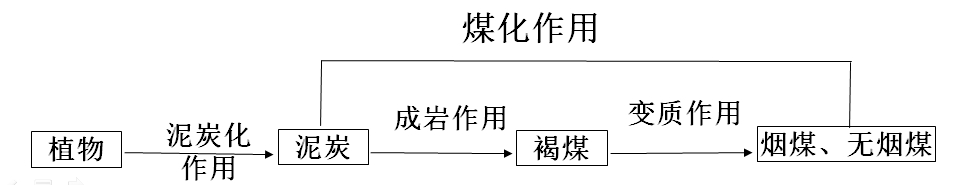
\includegraphics[scale=0.6]{1}
\caption{煤要经历的过程}

\end{figure}
\begin{figure}[h]
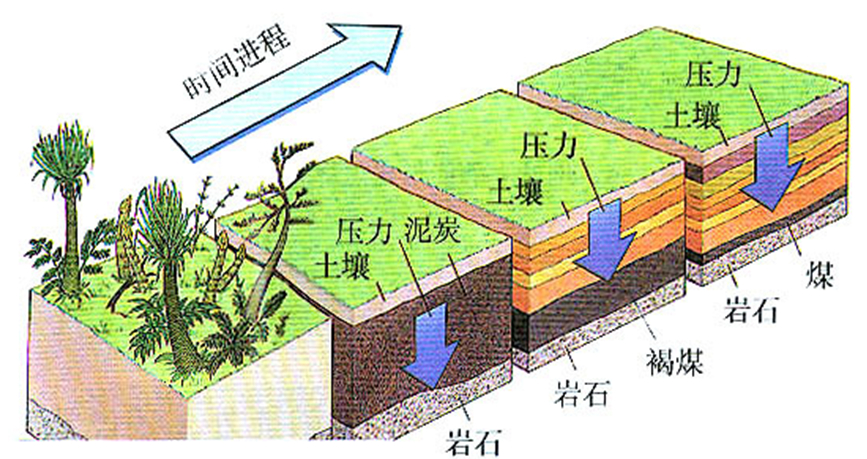
\includegraphics[scale=0.6]{2}
\caption{煤要经历的过程}
\end{figure}
根据成煤植物的不同,将煤分为腐植煤和腐泥煤两大类。\par
高等植物残骸在沼泽中经过生物化学作用,形成泥炭(一种松软的有机物);低等植物和浮游生物的残骸在缺氧条件下,经过厌氧分解,聚合和缩合作用形成腐泥,一种黑褐色的有机物(类似于污泥) \par
高等植物:包括苔藓、蕨类、裸子植物和被子植物。高等植物由低等植物长期进化而来,构造复杂,有根、茎、叶的区别。\par
低等植物:包括菌类和藻类,是由单细胞和多细胞构成的丝状体或叶状体植物,没有根、茎、叶等器官的分化。\par
泥炭和腐泥不断被上面的沉积物所覆盖,埋藏到一定深度后,在压力和温度的作用下,经过物理化学过程,分别形成腐植煤(褐煤、烟煤和无烟煤)和腐泥煤(腐泥褐煤、腐泥烟煤和腐泥无烟煤) 。\par
\subsection{煤的显微组分}
显微组分是指煤在显微镜下能够区别和辨识的最基本的组成成分,是显微镜下能观察到的煤中成煤原始植物残体转变而成的有机成分。煤的显微组分按其成因和工艺性质的不同,大致可分为镜质组、壳质组和惰质组三大类。    \par
\paragraph{镜质组}
   镜质组是由植物木质纤维组织受凝胶化作用转化形成的,是煤中最常见和最重要的显微组分组。
\paragraph{壳质组}
   壳质组包括孢子体、胶质体、木栓质体、藻类体和壳屑体等显微组分,来源于植物的孢子、角质层、木栓、树脂、蜡、脂肪和油。
\paragraph{惰质组}
   惰质组包括微粒体、粗粒体、半丝质体、丝质体、菌类体和惰屑体等显微组分。

\subsection{煤中的矿物质}

   煤是由有机成分和无机成分组成的。煤的有机成分是指煤的显微组分,是人们关注的中心。煤的无机成分是指在显微镜下能观察到的煤中矿物,以及与有机质相结合的各种金属、非金属元素和化合物。\par
按成因划分,煤中矿物质可分为三类。
\begin{itemize}
\item 植物成因的原生矿物质:来自原始植物的无机成分。
\item 陆源碎屑成因的矿物质:煤化作用第一阶段或煤矿床形成时由水或风带入其中的无机成分。
\item 化学和生物化学成因的矿物质:煤化作用第一阶段的同生-成岩矿物和煤化作用第二阶段形成的次生、后生矿物。
\end{itemize}
按矿物成分和性质,可将煤中矿物质分成以下几种类型。
\begin{itemize}

\item 粘土类矿物:常见的粘土类矿物有高岭石、水云母、伊利石等。
\item 硫化物类矿物:此类矿物包括黄铁矿、白铁矿等。
\item 碳酸盐类矿物:主要包括方解石和菱铁矿。
\item 氧化物类矿物:氧化物类矿物主要是石英等。
\item 硫酸盐类矿物:硫酸盐类矿物主要是石膏 。
\end{itemize}

\subsubsection{煤的岩石类型}
\paragraph{腐植煤的煤岩类型} 腐植煤煤层通常由镜煤(光亮条带)、亮煤(半光亮条带)、暗煤(黯淡条带)和丝炭(矿物木炭)所组成。其中镜煤和丝炭是最简单的煤岩类型,亮煤和暗煤是复杂的煤岩类型。
\subparagraph{镜煤} 镜煤呈黑色、深黑色,光泽强,明亮如镜,是煤中最颜色最深、光泽最强的类型,镜煤的挥发分和氢含量高,粘结性强,矿物质含量一般较少。
\subparagraph{亮煤} 亮煤是煤中最常见的煤岩类型。其光泽仅次于镜煤,性较脆,亮煤的各种物理、化学和工艺性质多介于镜煤和暗煤之间。
\subparagraph{暗煤}  暗煤的颜色为灰黑、暗黑,光泽暗淡,致密坚硬,韧性较大,密度大。一般富含壳质组的暗煤,往往略带油脂光泽,挥发分和氢含量高,粘结性好;富含惰质组分的暗煤略带丝绢光泽,挥发分低,粘结性差;富含粘土矿物的暗煤,则密度大、灰分高。
\subparagraph{丝炭} 丝炭外观像木炭,颜色灰黑或暗黑,具有明显的纤维状结构和丝绢光泽,疏松多孔,性脆易碎染指,丝炭在煤层中,一般数量不多。

\subsubsection{腐泥煤的煤岩类型} 腐泥煤是由低等植物和浮游生物经过部分腐解而成的煤。腐泥煤在显微镜下以其缺乏层理而区别于腐植煤。腐泥煤呈均一状结构,强度很大。低级腐泥煤的化学特征是氢含量和挥发分高,干馏时气体和焦油产率高。腐泥煤可分为烛煤和藻煤。
\subparagraph{烛煤} 宏观上烛煤为黑色,暗淡,有时具有弱油脂光泽。均一致密,贝壳状断口,韧性大。肉眼难以区分烛煤和藻煤。镜下烛煤一般显示规则的显微层理,几乎不含藻类体,但含非常丰富的孢子体,因而常被称为“孢子煤”。碎屑多,大小相近。烛煤易燃,燃烧时发出明亮的火焰,像蜡烛一样。烛煤的挥发分、氢含量和焦油产率较高。

\subparagraph{藻煤}     藻煤光泽暗淡,均一块状,贝壳状断口,韧性较大,灰分低时密度小,易燃,有沥青味。宏观上藻煤可以据其淡褐色和褐色条痕而区别于烛煤。显微镜下,显微组成以密集的藻类体为主,显微层理不明显。藻煤挥发分、氢含量和焦油产率高,有时灰分也高。

\subsubsection{煤的光泽岩石类型}
    煤岩类型是煤的岩石分类的基本单位。一般按平均光泽强度把煤的光泽岩石类型依次划分为光亮煤、半亮煤、半暗煤和暗淡煤四种基本类型。
\subparagraph{光亮煤}  主要由镜煤和亮煤组成,光泽很强。由于成分均一,条带状结构不明显。内生裂隙发育,脆度较大,机械强度小,易破碎,常具有贝壳状断口,镜煤和亮煤占组成的75\%以上,暗煤和丝炭少量或没有。粘结性较好,煤质好。
\subparagraph{半亮煤} 镜煤和亮煤含量在50\%$\sim$75\%之间,暗煤和丝炭含量较少,光泽也较强,最大的特点是条带状结构明显,内生裂隙较发育,常具有棱角状断口或阶梯状断口,是煤中常见的煤岩类型,煤质较好。
\subparagraph{半暗煤} 是由暗煤和亮煤组成,镜煤和亮煤含量在25\%$\sim$50\%之间,丝炭含量也较多。光泽较弱,硬度和韧性大,条带状、线理状或透镜状结构。内生裂隙不发育,断口参差不齐,矿物质含量常常较高,煤质较差。
\subparagraph{暗淡煤}  主要由暗煤和丝炭组成,镜煤和亮煤含量小于25\%。光泽暗淡,通常呈块状构造,致密、坚硬、韧性强,层理不明显,呈粒状结构,断口呈棱角状或参差状,矿物质含量往往很高,煤质差。

\section{煤的性质}
\subsection{煤的工业分析}
\subsubsection{煤中的水分} 煤中的水分可分为游离水和化合水。\par
    煤中游离水是指与煤呈物理态结合的水,它吸附在煤的外表面和内部孔隙中。因此,煤的颗粒越细,内部孔隙越发达,煤中吸附的水分就越高。煤中游离水分可分为两类:即在常温的大气中易于失去的水分和不愿失去的水分。前者吸附在煤的外表面和较大的毛细孔隙中,称为外在水分,用Mf表示;后者则存在于较小的孔隙中,称为内在水分,用Minh表示。煤的内在水分和外在水分质量之和就是煤的全水分,用Mt或Mar表示。\par
        外在水分和内在水分构成煤的全水分,它们的关系可用下式表示。
        $$M_{ar}=M_{inh}+M_{f}$$
        煤的化合水包括结晶水和热解水。结晶水是指煤中含结晶水的矿物质所具有的,如石膏(CaSO$_4$·4SiO$_2$·4H$_2$O)中的结晶水,通常煤中结晶水含量不大;热解水是煤炭在高温热解条件下,煤中的氧和氢结合生成的水,它取决于热解的条件和煤中的氧含量。通常,如果不作特殊说明,煤中的水分均是指煤中游离态的吸附水。
\subsubsection{煤的灰分}
 \paragraph{灰分}  将煤在815℃的条件下完全燃烧后所得的残渣为煤的灰分,用A表示。测定灰分时所用的煤样是粒度小于0.2mm的空气干燥基煤样,因此测定结果是空气干燥基的灰分产率,用Aad表示。
 \paragraph{煤中的矿物质} 煤中的矿物质是煤中的无机物的总称,包括在煤中独立存在的矿物质(高岭土、蒙脱石、硫铁矿、方解石、石英等),也包括与煤的有机质结合的无机元素,此外,煤中还有许多微量元素。
 \paragraph{煤灰成分} 煤灰是煤中矿物质在燃烧后形成的残渣。一般用主要元素的氧化物形式表示,如\chemfig{SiO_2}、\chemfig{Al_2O_3}、\chemfig{CaO}、MgO、\chemfig{Fe_2O_3}、\chemfig{TiO_2}、\chemfig{K_2O}、\chemfig{Na_2O}、\chemfig{SO_3}、\chemfig{P_2O_5}。 其中,最主要的是\chemfig{SiO_2}、\chemfig{Al_2O_3}、CaO、MgO、\chemfig{Fe_2O_3}几种,一般占95\%以上。
 \paragraph{煤灰熔融性} 煤灰熔融性是指煤灰在高温条件下软化、熔融、流动时的温度特性。通常用三个特征温度表示。
变形温度(DT)—煤灰锥体尖端开始弯曲或变圆时的温度。
软化温度(ST)—煤灰锥体弯曲至锥尖触及底板变成球形或半球形时的温度。
流动温度(FT)—煤灰锥体完全熔化展开成高度小于1.5mm薄层时的温度。
一般以煤灰软化温度ST作为衡量煤灰熔融性的指标。
\paragraph{煤中的微量元素} 在煤的矿物质和有机质中,除了上述含量较高的元素外,还含有含量较少的元素,即微量元素。从煤中提取稀有元素是重点研究的问题。一般来说,煤中锗含量达到20g/t以上、镓含量达到30g/t以上、铀含量达到300g/t以上、钍含量达到900g/t以上、铼含量达到2g/t以上就有工业利用价值。煤中常见的微量元素主要有锗、镓、铀、钒、铍、铼、钍、钛等。
\paragraph{煤中的有害元素} 煤中的有害元素主要有硫、磷、氯、砷、氟、汞、铍、镉、铅等 。
\subsubsection{挥发分和固定炭} 在高温(900℃)条件下,将煤隔绝空气加热一定时间,煤的有机质发生热解反应,形成部分小分子的化合物,呈气态析出,其余有机质则呈固体形式残留下来。由有机质热解形成并呈气态析出的化合物称为挥发物,该挥发物占煤样质量的百分数称为挥发分。以固体形式残留下来的有机质占煤样质量的百分数称为固定炭。挥发分用V表示,固定炭用FC表示。\par
挥发分和固定炭有如下关系:$$FCad=100-Mad-Aad-Vad$$
\subsection{煤的元素分析} 煤的元素分析是对组成煤的有机质主要元素的化验分析。煤的有机质主要由碳、氢、氧、氮和硫等五种元素组成。
\subsubsection{煤中的碳元素} 碳是构成煤分子骨架的最重要元素之一,也是煤燃尽过程中放出热能最主要的元素之一。随煤化程度的提高,煤中碳元素逐渐增加,腐植煤的碳含量高于腐泥煤,在不同煤岩组分中,碳含量的顺序是:惰质组>镜质组>壳质组。
\subsubsection{煤中的氢元素} 元素是煤中第二重要的元素,主要存在于煤分子的侧链和官能团上,在有机质中的含量约为2.0\%$\sim$6.5\%左右,我国无烟煤分类中采用氢元素含量作为分类指标。氢元素的发热量约为碳元素的四倍,虽然含量较低,但氢元素的变化对煤的发热量影响很大。腐泥煤的氢含量高于腐植煤,在不同煤岩组分中,氢含量的顺序是:壳质组>镜质组>惰质组。
\subsubsection{煤中的氧元素} 氧也是组成煤有机质的重要元素,主要存在于煤分子的含氧官能团上。随煤化程度的提高,煤中氧元素迅速下降,氧元素在燃烧时不产生热量,在煤液化时要消耗氢气,对煤的利用不利。腐植煤的含氧量高于腐泥煤,在不同煤岩组分中,氧含量的顺序是:镜质组>惰质组>壳质组。
\subsubsection{煤中的氮元素} 煤中的氮元素含量较少,一般为0.5\%$\sim$1.8\%,与煤化程度无规律可循。它主要来自成煤植物的蛋白质。煤中氮在燃烧时也不放热,主要以N$_2$的形式进入废气,少量形成NOx。当煤在炼焦时,煤中的氮部分形成NH$_3$、HCN及其它有机含氮化合物,其余的则留在焦炭中。
\subsubsection{煤中的硫元素} 硫是煤中主要的有害元素,在煤的焦化、气化和燃烧中均生成对工艺和环境有害的H2S和SO2等物质。\par
    煤中硫来源有两种:一是成煤植物本身所含的硫—原生硫,另一种是来自成煤环境及成岩变质过程中加入的硫—次生硫。对绝大多数煤来说,其中的硫主要来自次生硫。\par
 煤中的硫分为有机硫和无机硫。有机硫存在于煤的有机质分子上,分布均匀,极难脱除。无机硫主要以硫铁矿、硫酸盐等形式存在,其中以硫铁矿硫居多。一般情况下,煤中的硫酸盐硫是黄铁矿氧化所致,因而未经氧化的煤中的硫酸盐硫含量很少。\par
    煤中的有机硫用So表示,硫铁矿硫用Sp表示,硫酸盐硫用Ss表示,有机硫和无机硫之和称为煤的全硫,用St表示,即$$S_t=S_o+S_p+S_s$$

\subsection{煤质分析中的基准及其相互换算}
\subsubsection{基准的基本概念} 大量的分析指标是用百分比表示的,计算百分比时,有一个计算的基准。某个指标的百分数是指它占某种具体对象的百分数,这个对象就是基准。
\subsubsection{煤质分析中不同基准的物质含义}
煤质分析时煤炭组成有两种划分法,一种是将煤划分为有机质(用挥发分V、固定炭FC或C、H、O、N和St近似代替)和无机质(水分M、矿物质MM),另一种是将煤划分为可燃质(挥发分V、固定炭FC或C、H、O、N和St)和不可燃质(水分M、灰分A)。各种基准的划分含义如下:    \\
空气干燥基(分析基ad):
\begin{eqnarray}
 M_{ad}+A_{ad}+V_{ad}+FC_{ad}=100\%  \\(OR)
 M_{ad}+A_{ad}+C_{ad}+H_{ad}+O_{ad}+N_{ad}+S_{t,ad}=100\%
\end{eqnarray}
干燥基(干基d):

\begin{eqnarray}
A_d+V_d+FC_d=100 \%  \\ (OR)
A_d+C_d+H_d+O_d+N_d+S_{t,d}=100\%
\end{eqnarray}
干燥无矿物质基(有机基dmmf):
\begin{eqnarray}
A_d+V_d+FC_d=100 \%  \\ (OR)
A_d+C_d+H_d+O_d+N_d+S_{t,d}=100\%
\end{eqnarray}

\begin{eqnarray}
V_{dmmf}+FC_{dmmf}=100\% \\
(OR)C_{dmmf}+H_{dmmf}+O_{dmmf}+N_{dmmf}+S_{t,dmmf}=100\%
\end{eqnarray}
\begin{eqnarray}
V_{daf}+FC_{daf}=100\% \\
          (OR)C_{daf}+H_{daf}+O_{daf}+N_{daf}+S_{t,daf}=100\%
\end{eqnarray}
收到基(ar):
\begin{eqnarray}
          M_{ar}+A_{ar}+V_{ar}+FC_{ar}=100\%\\
          (OR)M_{ar}+A_{ar}+C_{ar}+H_{ar}+O_{ar}+N_{ar}+S_{t,ar}=100\%
\end{eqnarray}
煤质基准间相互关系如下图
\begin{figure}[h]
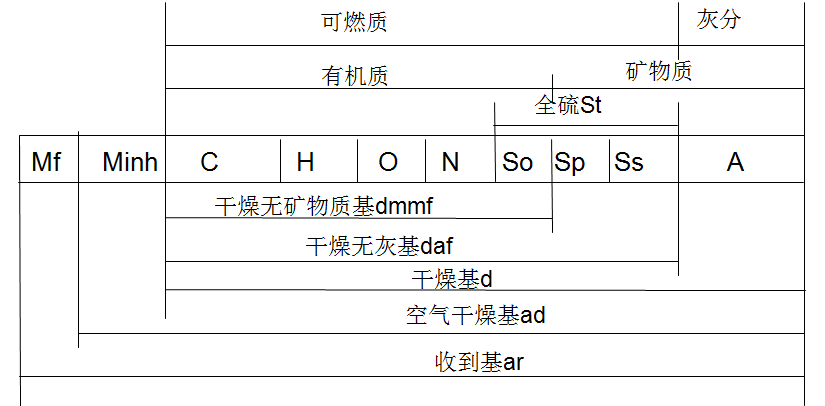
\includegraphics[scale=0.6]{3}
\caption{煤要经历的过程}

\end{figure}
\subsubsection{各基准间的相互换算}
\begin{figure}[h]
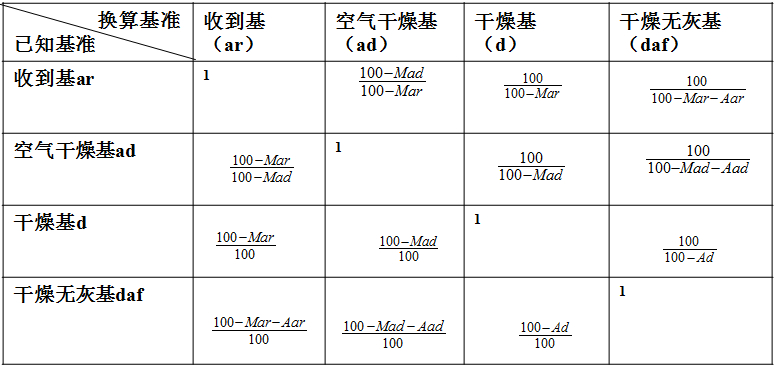
\includegraphics[scale=0.7]{4}
\caption{各基准间的相互换算}

\end{figure}
%%%%%%%%%%%%%%%%%%%%%%%%%%%%%%%%%%%%%%%%%%%%%%%%%
\subsection{煤的物理性质和工艺性质}
\subsubsection{煤的物理性质}
煤的物理性质包括:煤的机械性质(密度和硬度)、光学性质、电磁性质和煤的热稳定性等。
\paragraph{煤的密度}
可分为:真密度(TRD)、视密度(ARD)和堆积密度(BRD)。

  $$ \mbox{孔隙度}=\dfrac{TRD-ARD}{TRD}\%$$

\paragraph{煤的机械性质}
是指煤在机械力作用下所表现出来的各种特性,如硬度、脆度、可磨性等,这些性质对煤的开采、破碎、燃烧、气化和成型等工艺过程有实用意义。
\paragraph{煤的热稳定性}  是指块煤在高温下保持原来粒度的能力,用TS表示。一般褐煤的稳定性最差,其次是无烟煤,烟煤较好。
\subsubsection{煤的工艺性质}
\paragraph{煤的发热量} 也称煤的热值,是指单位质量的煤完全燃烧后所释放出的热能,用KJ/g或MJ/g表示。一般采用氧氮法测定煤的发热量,用Q$_{b,ad}$表示,即弹筒发热量。为了得到接近实际的发热量值,需对弹筒发热量进行校正,发热量均是指恒容发热量。
\subparagraph{弹筒发热量与恒容高位发热量的校正}  从弹筒发热量中扣除稀硫酸和稀硝酸生成热,称为恒容高位发热量,简称高位发热量,用Q$_{gr,v,ad}$表示,计算公式如下:
$${Q_{gr,v,ad}=Q_{b,ad}-(95S{_{b,ad}}+\alpha *Q_{b,ad})}$$
\begin{flushleft}




~~~~~~~~~~~$Q_{gr,v,ad}$—空气干燥基的恒容高位发热量,J/g;\\
~~~~~~~~~~~$Q_{b,ad}$—空气干燥基的弹筒发热量,J/g;\\
~~~~~~~~~~~$S_{b,ad}$—由弹筒洗液测得的硫含量\%,\\ 满足下列条件之一时可用全硫代替:\\
~~~~~~~~~~~$Q_{b,ad}$>14.6KJ/g  或  $S_{b,ad}$<4\%\par
 ~~~~~~~~~~~   $\alpha$ —硝酸生成热校正系数。\\试验证明,$\alpha$  与$Q_{b,ad}$有关,取值如下:\\
   ~~~~~~~~~~~    $Q_{b,ad}$ $\leq$16.7KJ/g时,$\alpha$ =0.0010; \\
   ~~~~~~~~~~~     16.7KJ/g$<$ $Q_{b,ad}$ $\leq$25.10KJ/g时,$\alpha$=0.0012\\
   ~~~~~~~~~~~   $Q_{b,ad}$>25.1 KJ/g时,$\alpha$  =0.0016 \\

\end{flushleft}
\subparagraph{弹筒发热量与恒容低位发热量的校正}  从恒容高位发热量中扣除水(煤种的吸附水合氢燃烧生成的水)的汽化热,称为恒容低位发热量,简称低位发热量,用符号Q$_{ent,v,ad}$表示,计算公式如下:
$$Q_{ent,v,ad}=Q_{gr,v,ad}-206H_{ad}-23M_{ad}$$
\begin{flushleft}




~~~~~~~~~~~$Q_{ent,v,ad}$——空气干燥基的恒容低位发热量,J/g;\\
~~~~~~~~~~~$Q_{gr,v,ad}$——空气干燥基的恒容高位发热量,J/g;\\

~~~~~~~~~~~$M_{ad}$——空气干燥基的水分,\%;\\
 ~~~~~~~~~~~$H_{ad}$——空气干燥基的氢含量,\%;\\
   ~~~~~~~~~~~    206—0.01g氢生成水的汽化热,J;\\

   ~~~~~~~~~~~     23—0.01g吸附水的汽化热,J。


\end{flushleft}
\paragraph{煤的粘结性和结焦性}
煤的粘结性是指煤在干馏时产生的胶质体粘结自身和惰性物料的能力。煤的结焦性是指单种煤或配和煤在工业焦炉或模拟工业焦炉的炼焦条件下,粘结成块并最终形成具有一定块度和强度的焦炭的能力。粘结性是结焦性的必要条件,而煤的塑性、流动性、膨胀性、透气性、热稳定性等对煤的结焦性也有较大的影响。\par
煤的粘结性和结焦性的评定方法主要有以下几种。
\begin{itemize}
\item  罗加指数:用RI表示。
\item  粘结指数:用G表示。
\item  胶质层指数:以胶质层最大厚度Y值表示。
\item 奥亚膨胀度 :用b表示。
\item  坩埚膨胀序数:用CNS表示。
\end{itemize}

\section{中国煤炭分类}
中国煤炭分类国家标准是1989 年 10 月 1 日正式实行的,它具有广泛的实用性、科学性和权威性 , 为煤炭的合理利用及不同煤种比价合理的调整提供了技术依据。
\subsection{分类方案 }
分类方案首先根据表征煤化程度的干燥无灰基挥发分 V$_{daf}$(\%), 将所有煤炭按 V$_{daf}$ 《 10\% 、 V$_{daf}$>10\%$\sim$20\% 、  V$_{daf}$>20\% $\sim$28\% 、  V$_{daf}$>28\%$\sim$37\% 和  V$_{dd}$>37\% 共分为五部分,再分别根据透光率或粘结指数等其它指标把各类煤再细分为褐煤、烟煤和无烟煤三部分。     \par
在褐煤阶段,利用透光率 (P$_m$,\%) 和恒湿无灰基煤的高位发热量 (Q$_{gr,maf}$, MJ/Kg) 来区分褐煤和长焰煤,并用 PM 再把褐煤细分为两小类。\par
    在烟煤阶段,利用粘结指数 (G) 和胶质层最大厚度 Y 值(mm)( 或奥亚膨胀度 b值 ,\%) 再细分为 12 类煤。\par
    在无烟煤阶段,根据氢含量 (H$_{daf}$,\%) 或挥发分 (V$_{daf}$,\%) 再细分为 3 小类。\par
 \begin{figure}[!ht]
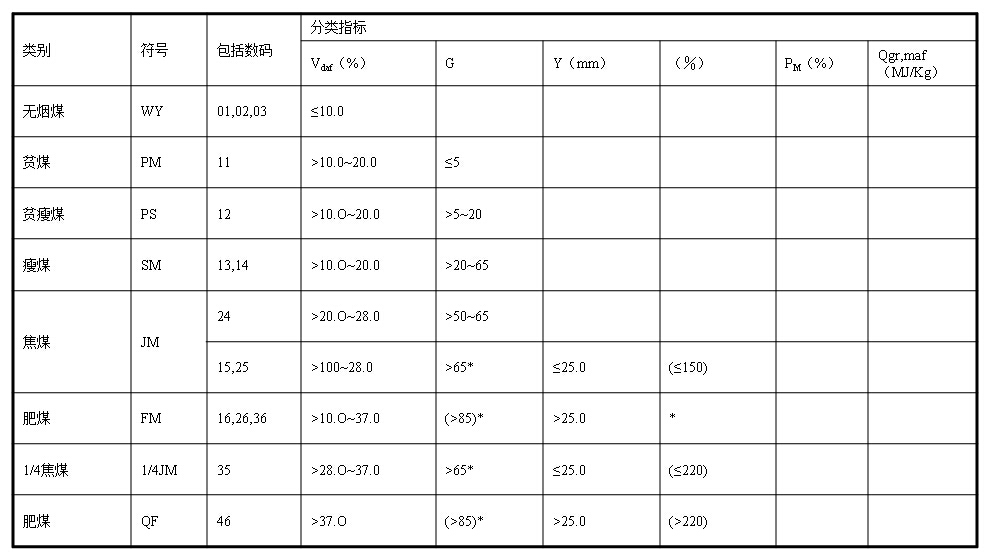
\includegraphics[scale=0.6]{5}
\caption{中国煤炭分类简表1}
\end{figure}
 \begin{figure}[!ht]
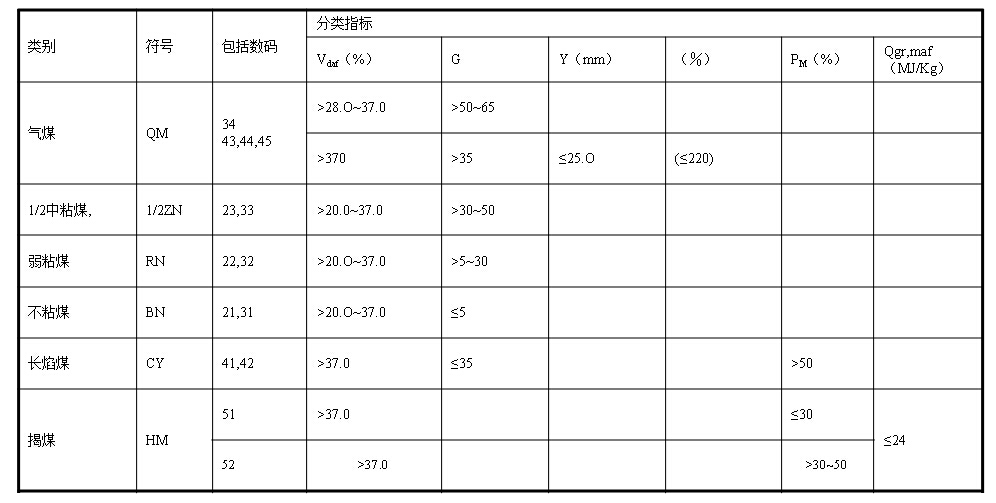
\includegraphics[scale=0.6]{6}
\caption{中国煤炭分类简表2}
\end{figure}
\subsection{各类煤的基本特性及其主要用途}
\subparagraph{无烟煤(WY):}特点是固定碳高 , 挥发分低 , 纯煤真密度高达1.35$\sim$1.90, 无粘结性 , 燃点高 , 一般达 360$\sim$420 ℃左右。燃烧时冒烟少。这类煤又细分为 01 号 ( 年老 )、02 号 ( 典型 ) 和 03 号 ( 年轻 ) 三个小类。\par
无烟煤主要供民用和作合成氨造气的原料;低灰、低硫,且质软易磨的无烟煤,不仅是理想的高炉喷吹和烧结铁矿石用的还原剂与燃料,而且还可以作制造各种碳素材料如碳电极、炭块,阳报糊和活性炭、滤料等原料;某些无烟煤制成的航空用型煤还可用于飞机发动机和车辆马达的保温。
\subparagraph{贫煤 (PM):}是烟煤中变质程度最高的一小类煤,不粘结或呈微弱的粘结,在层状焦炉中不结焦。发热量比无烟煤高,燃烧时火焰短 , 耐烧,, 但燃点也较高,仅次于无烟煤,一般在 350$\sim$360 ℃ 左右。主要代为电厂燃料,尤其是与高挥发分煤配合燃烧时更能充分发挥其热值高又耐烧的优点。一般也可作民用及工业锅炉的燃料。
\subparagraph{贫瘦煤 (PS):} 是炼焦煤中变质程度最高的一种 , 其特点是挥发分较低 , 但其粘结性仅次于典型瘦煤。单独炼焦时,生成的粉焦多; 在配煤炼焦时配人较少比例时也能起到瘦煤的瘦化作用,对提高焦炭的块度起到良好的作用。这类煤也是发电机车、民用及工业炉窑的燃料。
\subparagraph{瘦煤(SM):} 是具有中等粘结性的低挥发分炼焦煤。炼焦过程中能产生相当数量的胶质体 ,Y 值一般在 6$\sim$10mm 左右。单独炼焦时能得到块度大、裂纹少、抗碎强度较好的焦炭,但其耐磨强度较差,其作为配煤炼焦使用较好。高硫、高灰的瘦煤一般只作电厂及锅炉燃料。
\subparagraph{焦煤 (JM):}焦煤 (JM):是一种结焦性较强的炼焦煤 , 挥发分 (Vdaf) 一般在16\%$\sim$28\% 之间。加热时能产生热稳定性很高的胶质体。单独炼焦时能得到块度大、裂纹少,抗碎强度和耐磨强度都很高的焦炭。但单独炼焦时膨胀压力大有时易产生推焦困难。一般以作为配煤炼焦使用较好。
\subparagraph{肥煤 (FM):}是中等挥发分及中高挥发分的强粘结性炼焦煤,其挥发分多在 25\%$\sim$35\% 左右。加热时能产生大量的胶质体。单独炼焦时能生成熔融性好、强度高的焦炭,耐磨强度比相同挥发分的焦煤炼出的焦炭还好。它是配煤炼焦中的基础煤。但单煤炼焦时炼出的焦炭有较多的横裂纹,焦根部分常有蜂焦。
\subparagraph{1/3 焦煤 (1/3JM):} 是中等偏高挥发分的较强粘结性炼焦煤,它实质上是一种介于焦煤、肥煤和气煤之间的过渡煤。在单煤炼焦时能生成熔融性良好,强度较高的焦炭。焦炭的抗碎强度接近肥煤,耐磨强度则又明显地高于气肥煤和气煤。因此它既能单煤炼焦供中型高炉使用,也是良好的配煤炼焦的基础煤。在炼焦时配入量可在较宽范围内波动而能获得高强度的焦炭。
\subparagraph{气肥煤 (QF) } 气肥煤是一种挥发分和胶质体厚度都很高的强粘结性炼焦煤。结焦性高于气煤而低于肥煤,胶质体虽多但较稀薄 ( 即胶质体的粘稠度小 )。单煤炼焦时能产生大量的煤气和液体化学产品。最适合于高温制造城市煤气,也可用于炼焦以增加化学产品的产率。
\subparagraph{气煤(QM)} 气煤是一种变质程度较低,挥发分较高的炼焦煤,结焦性较强,加热时能产生较高的煤气和较多的焦油。胶质体的热稳定性较差,也能单独结焦。但焦炭的抗碎强度和耐磨强度多低于其它炼焦用煤牌号。焦炭多呈细长条而易碎,并有较多的纵裂纹。一般在配煤炼焦时多配入气煤后可增多煤气和化学产品的产率。有的气煤也可单独高温干馏来制造城市煤气。
\subparagraph{10、1/2 中粘煤 (1/2ZN):} 是一种过渡煤。但这类煤的储量和产量不多。可作为配煤炼焦的原料。但单煤炼焦时的焦炭强度差,粉焦率高。故主要可作为气化或动力用煤。我国目前尚未发现单独生产1/2中粘煤的矿井。
\subparagraph{弱粘煤 (RN)} 是一种粘结性较弱的从低变质到中等变质程度的非炼焦用烟煤。隔绝空气加热时产生的胶质体少,炼焦时有的能结成强度差的小块焦,有的只有少部分能凝结成碎屑焦,粉焦率很高。一般适用于气化及动力燃料。
\subparagraph{不粘煤 (BN)} 是一种在成煤初期已经受到相当程度氧化作用的低变质到中等变质程度的非炼焦用烟煤。焦化时不产生胶质体。煤的水分大,纯煤发热量仅高于一般褐煤而低于所有烟煤,煤中含氧量多在 10\%$\sim$15\% 左右。 主要可作为发电和气化用煤,也可作为动力和民用燃料,最好与其他煤类配合燃烧,可充分利用其低灰、低硫的优点。
\subparagraph{长焰煤 (CY)} 是变质程度最低的高挥发分非炼焦用烟煤,其煤化程度仅高于褐煤而低于其它各类烟煤。煤的燃点低,纯煤热值也不高。从无粘结性到弱粘结性均有,有的还含有一定数量的腐植酸。贮存时易风化、碎裂。有的长焰煤加热时能产生一定数量的胶质体,也能结成细小的长条形焦炭,但焦炭强度差,焦粉率高。一般不用于炼焦,作为电厂、机车燃料以及工业炉窑燃料。也可作气化用煤。
\section{中国煤质特征}
中国是世界第一产煤大国 , 但煤炭质量不甚理想。
\subsection{煤的硫分 } 中国煤中硫分的分布特点是南方煤田中部硫分较高,北方煤田则下部煤层的硫分较高;从不同煤化度煤的硫分看,总的趋势是低阶煤如褐煤、长焰煤、不粘煤和弱粘煤等动力用煤的硫分较低,炼焦煤中则以气煤的平均硫分最低,肥煤的硫分最高。高变质的贫煤和无烟煤的高硫煤比例也相对较多;按我国各地区煤储量划分的煤中硫分,西南区煤的平均硫分最高,S$_{t,d}$ 平均达1.61\%, 其次为中南区,S$_{t,d}$ 平均 1.04\%, 东北区煤的平均硫分最低,S$_{t,d}$ 为 0.36\%, 西北区煤的平均硫分也低至0.60\% 以下。按我国不同炼焦煤的储量平均硫分看,以焦煤的硫分最高,平均达1.65\%,其次为肥煤类,S$_{t,d}$ 平均为 1.41\%,气煤和1/3焦煤的硫分最低,S$_{t,d}$ 平均仅0.62\%。瘦煤和贫瘦煤的平均硫分也达1.2\%。 \par
从我国动力煤按储量的平均硫分看,以贫煤的硫分最高,S$_{t,d}$ 平均达1.67\%, 无烟煤的平均硫分也高至1.24\%, 但低阶煤如褐煤、不粘煤和长焰煤的平均硫分相对较低,S$_{t,d}$分别低至0.55\% 、0.60\%和0.75\%。
  \subsection{煤的灰分} 由中国煤种资源数据库的资料统计,中国生产矿区煤层和商品煤的平均灰分都在20\%以上,由于机采程度的不断提高,所以近年来毛煤的灰分也不断增高。在商品煤中,以炼焦精煤灰分最低,全国平均仅稍高于10\%;动力煤的平均灰分达25\% 以上,其中以发电用煤的平均灰分较高,Ad多在27\%$\sim$28\% 左右, 且有不少在30\% 以上甚至40\% 以上,仅少数电厂用煤的灰分在20\% 以下。
  \subsection{煤的发热量}
  的发热量大小除了与灰分有关以外 , 还与煤的类别有显著关系 , 如灰分相同的焦煤和褐煤之间 Q$_{g,daf}$ 值可相差 4$\sim$6MJ/kg 以上。由统计结果表明 , 中国褐煤的收到基低位发热量Q$_{net,ar}$r多在14.63MJ/kg(3500kcal/kg)以下,且其中不少在12.54MJ/kg(3000kcalAEg)以下。不粘煤和弱粘煤矿区商品煤的发热量大部较高,如大同、东胜 、神府等矿区煤的 Q$_{net,ar}$ 值平均在25.09MJ/kg(6000kcal/kg)以上,其中有不少可达29.4MJ/kg(7000kcal/kg)以上 , 最低的一般也在 20.91MJ/kg(5000kcal/kg)以上。无烟煤矿区在北方的一些矿井的发热量也普遍较高, 如阳泉三、四矿、晋城各矿的平均发热量Qnet,ar也都在24MJ/kg以上;炼焦煤的发热量则普遍较高,尤其是洗精煤的发热量Q$_{net,ar}$ 一般都在 25.09MJ/kg(6000kcal/kg) 以上,但洗煤厂的洗混煤和洗中煤的发热量Q$_{net,ar}$则普遍较低,多在 20.91MJ/kg(5000kcal/kg) 以下。
\subsection{中国煤的其它质量指标}
\subparagraph{煤的挥发分} 中国煤的平均挥发分较高, 由统计结果表明, 全国按储量划分时的平均挥发分 ( Vdaf) 约为 28\%, 其中Vdaf>28\%$\sim$37\% 的中高挥发分煤的比例约占 30\%,Vdaf>37\%$\sim$50\% 的高挥发分煤约占 25\%弱 ,Vdd>50\% 的特高挥发分煤的比例则不到1\%, 挥发分 (Vdaf) 低于10\% 的无烟煤的比例11\%,Vdaf=10\%$\sim$20\% 之间的低挥发分煤的比例约为 20\%。我国商品煤的平均挥发分约比原煤的降低 1\%$\sim$2\% 左右。
\subparagraph{煤的灰成分和灰熔融性}
通常煤灰中的 $Al_2O_3$含量较高 , 灰熔融性软化温度也较高。
\section{中国煤炭质量分级标准}
目前,已制订出十余项有关煤炭质量的分级标准,其中七项为国家标准 ( 或报批稿 ), 其余均为行业标准 ( 报批稿 ) 。
\subsection{煤灰分分级}
 \begin{figure}[!ht]
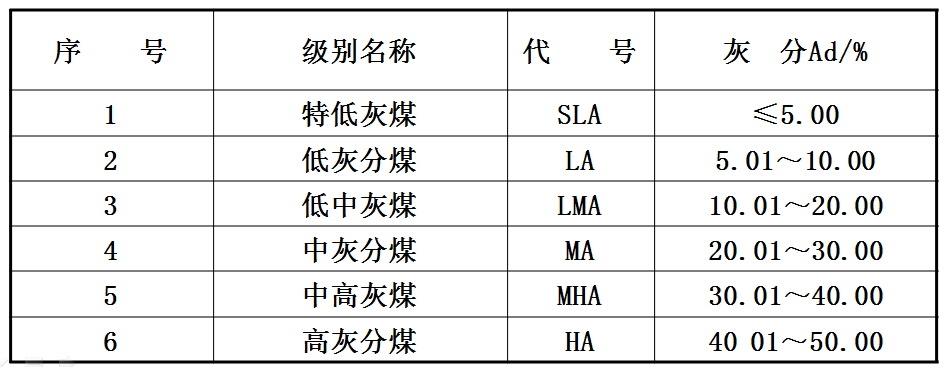
\includegraphics[scale=0.6]{7}
\caption{煤炭灰分分级标准 }
\end{figure}
\subsection{硫分分级}
 \begin{figure}[!ht]
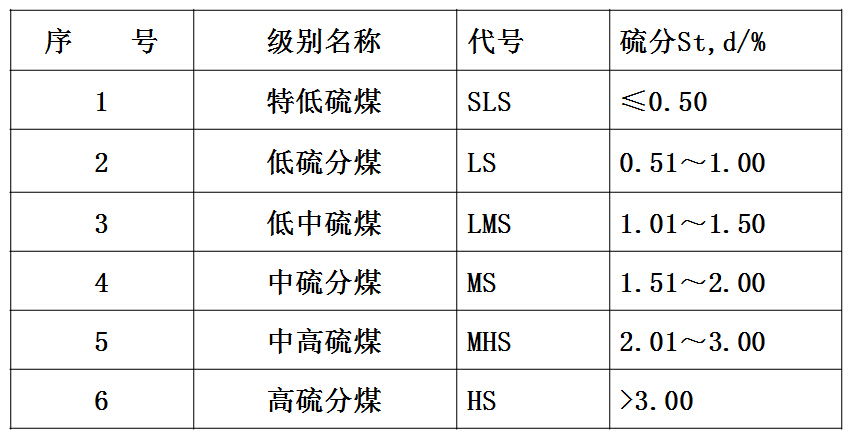
\includegraphics[scale=0.67]{8}
\caption{煤炭硫分分级标准}
\end{figure}
\subsection{煤炭发热量分级 }
 \begin{figure}[!ht]
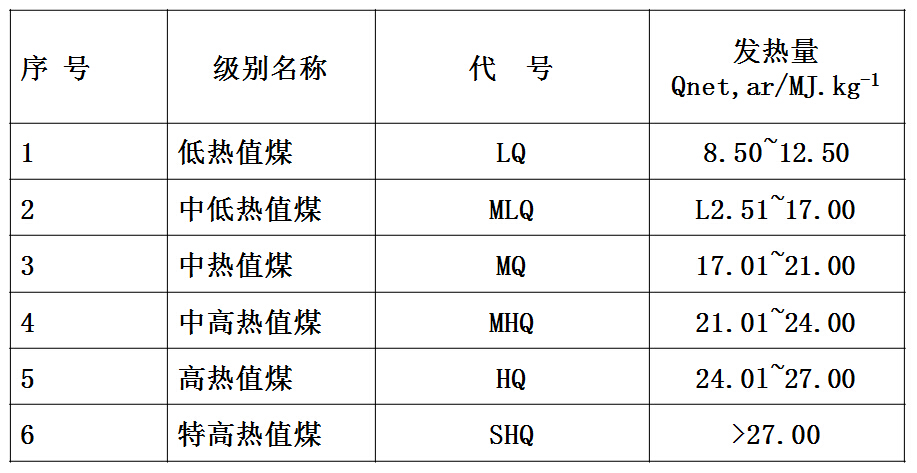
\includegraphics[scale=0.65]{9}
\caption{煤炭发热量分级标准}
\end{figure}
\subsection{煤的挥发分产率分级 }
 \begin{figure}[!ht]
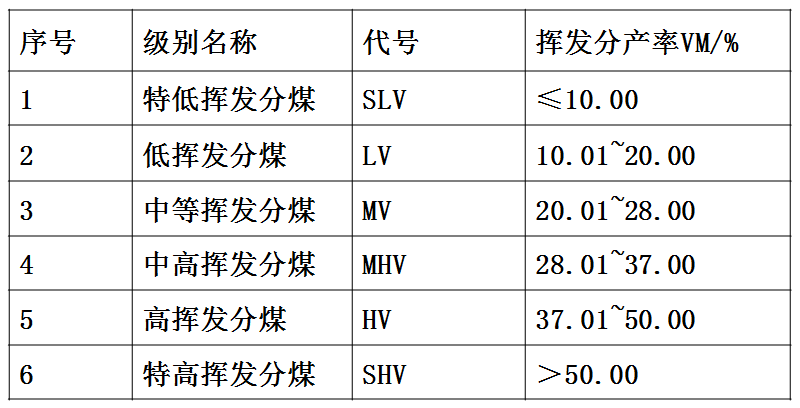
\includegraphics[scale=0.736]{10}
\caption{煤的干燥无灰基挥发分产率分级标准}
\end{figure}
\section{各种工业用煤质量指标}
煤炭既是燃料 , 也是卫业原料 , 广泛地用于冶金、电力、化 工、城市煤气、铁路、建材等国民经济各部门。不同的行业、不同的用煤设备对煤炭的质量均有不同的要求。
\subsection{炼焦用煤的质量要求}
 \begin{figure}[!ht]
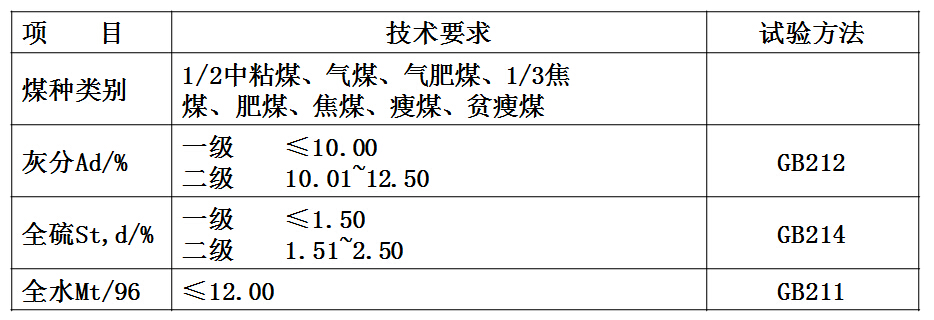
\includegraphics[scale=0.6]{11}
\caption{冶金焦用煤质量要求 }
\end{figure}


 \begin{figure}[!ht]
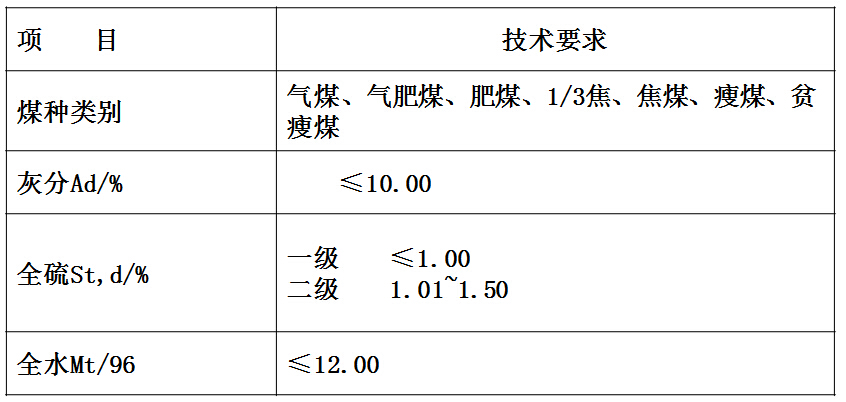
\includegraphics[scale=0.66]{12}
\caption{铸造焦用煤质量要求 }
\end{figure}
\subsection{发电用煤的质量要求}
 \begin{figure}[!ht]
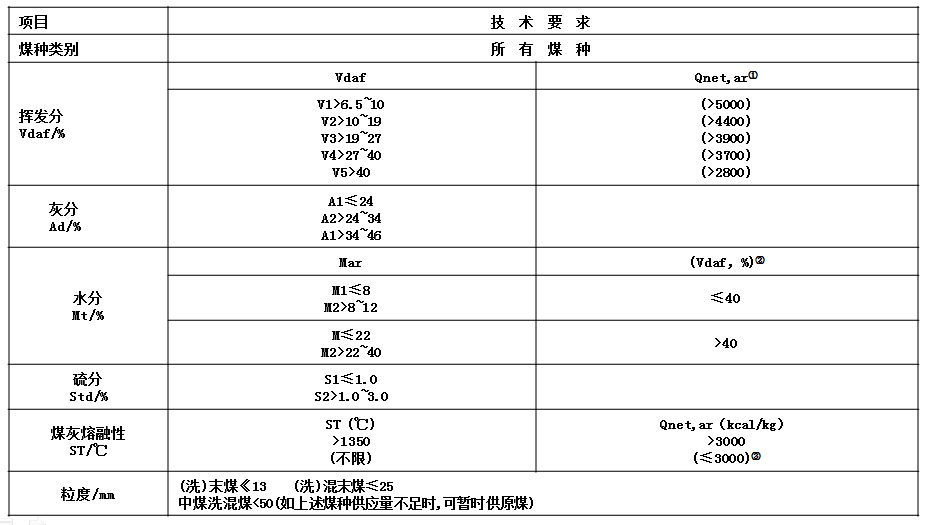
\includegraphics[scale=0.6]{13}
\caption{铸造焦用煤质量要求 }
\end{figure}

\subsection{气化用煤的质量要求}
 \begin{figure}[!ht]
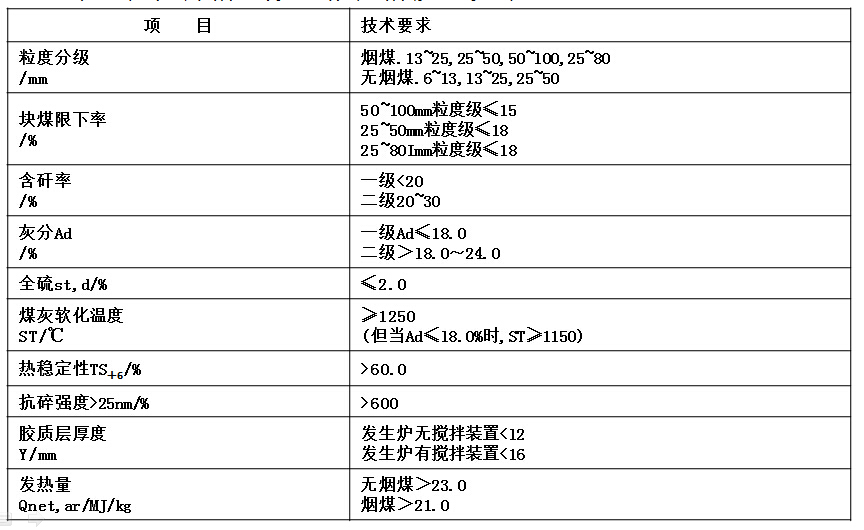
\includegraphics[scale=0.67]{14}
\caption{常压固定床煤气发生炉用煤质量要求  }
\end{figure}

 \begin{figure}[!ht]
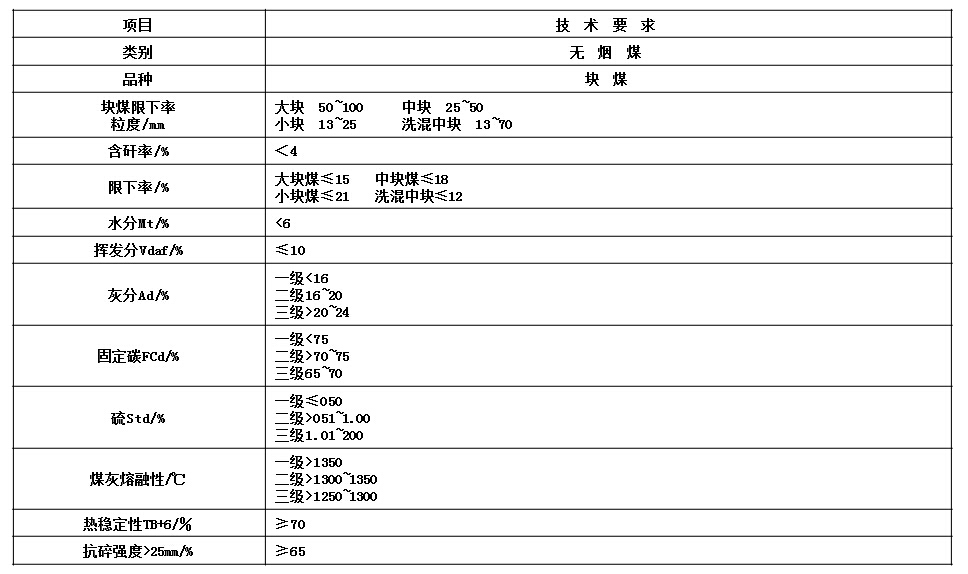
\includegraphics[scale=0.6]{15}
\caption{合成氨用煤质量要求 }
\end{figure}

\subsection{蒸汽机车用煤的质量要求}
 \begin{figure}[!ht]
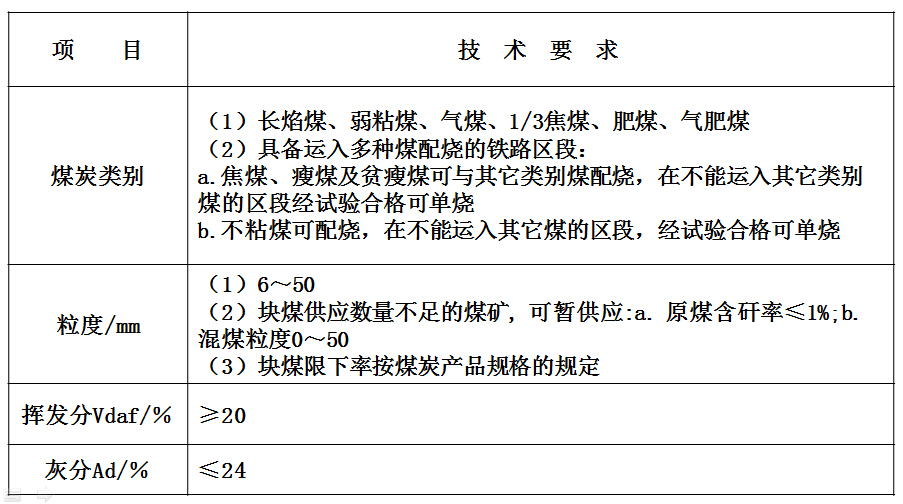
\includegraphics[scale=0.64]{16}
\caption{蒸汽机车用煤质量要求 }
\end{figure}

\subsection{水泥回转窑用煤的质量要求}
 \begin{figure}[!ht]
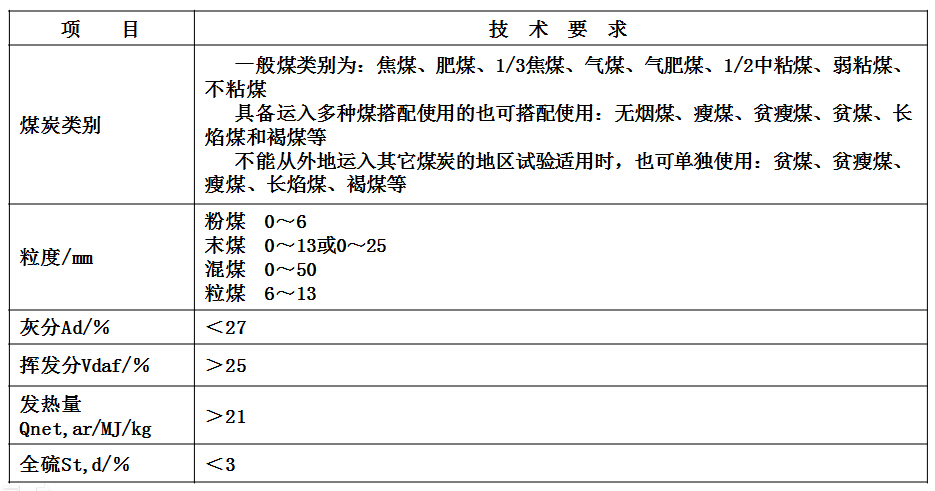
\includegraphics[scale=0.6]{17}
\caption{水泥回转窑用煤的质量要求}
\end{figure}

\subsection{高炉喷吹用无烟煤质量要求}
 \begin{figure}[!ht]
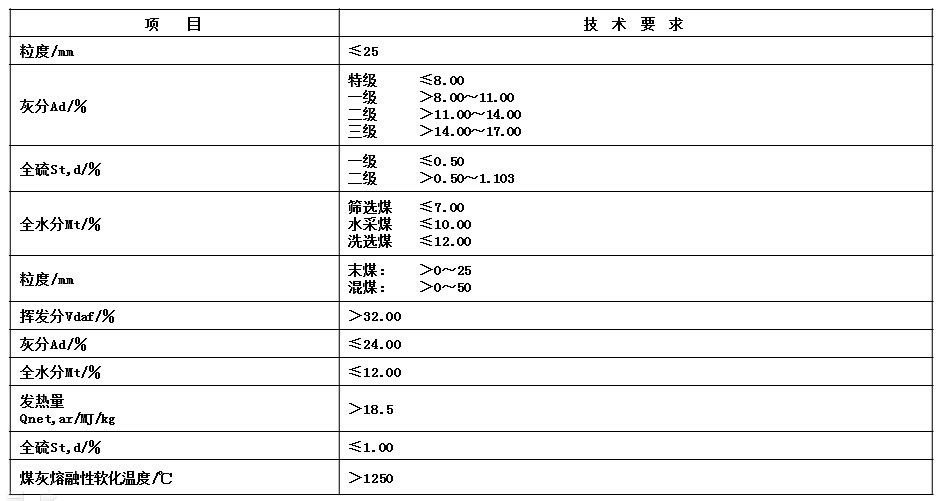
\includegraphics[scale=0.6]{18}
\caption{高炉喷吹用无烟煤质量要求}
\end{figure}

\chapter{煤炭洗选、脱硫与动力配煤}
\begin{itemize}
\item 本章主要讲述煤炭洗选加工、脱硫技术和动力配煤。
 \item 要求掌握动力配煤基本原理及其优化、动力配煤的固硫技术;
\item 熟悉煤炭洗选新工艺、新方法、新设备。
\item 了解贵州煤炭洗选现状及发展趋势。
\end{itemize}
\section{煤炭洗选加工现状}
\subsection{煤炭能源在我国的地位和作用}
我国是一个多煤少油的国家,已探明的煤炭储量占世界煤炭储量的33.8\%,可采量仅次于前苏联和美国,位居第三。我国煤产量位居世界第一位,出口量仅次于澳大利亚而居于第二位。煤炭在我国一次性能源结构中处于绝对主要位置,50年代的比例曾高达90\%。随着大庆油田、渤海油田的发现和开发,一次性能源结构才有了一定程度的改变,但煤仍然占到70\%以上。《中国可持续能源发展战略》研究报告中,20多位中科院和工程院院士一致认为,到2050年,煤炭所占比例不会低于50\%。可以预见,在未来几十年内,煤炭仍将是我国的主要能源和重要的战略物资,具有不可替代性,煤炭工业在国民经济中的基础地位,将是长期的和稳固的。 \par
    我国煤炭资源从开采、加工到消费的过程仍然是传统的经济模式,对煤炭的利用是粗放型的,在资源存量和环境承载两个方面承受着高强度的资源消耗和严重的环境污染。目前我国燃煤二氧化硫排放量占二氧化硫排放总量的90\%,粉尘对大气的污染还很严重。所以,我国在20世纪80年代中期启动了洁净煤技术,即以煤炭生产加工技术、煤炭燃烧技术、煤炭转化技术及污染控制技术为一体的技术体系。而煤炭洗选加工是洁净煤的源头技术,是国民经济可持续发展的重要条件。

\subsection{中国煤炭洗选加工现状}
中国选煤工艺从50-70年代的以跳汰、浮选为主,发展到80年代的跳汰粗选、重介旋流器精选、浮选流程,再到90年代的跳汰、重介分选、动筛跳汰选、风选、微泡浮选等工艺共存的状态。近几年,由于解决了介质回收、高效泵送、设备及其管道的耐磨等问题,重介选煤工艺的基建投资和生产成本不断降低,重介质选煤技术在我国得到了迅速发展,其易操作和高效率的特性越来越受到欢迎,并逐渐成为主导工艺。各种类型的重介质分选机、重介质旋流器已投入工业应用。如刮板重介分选机、三产品重介质旋流器、小直径重介质旋流器、大直径重介质旋流器等。\par
目前我国原煤入洗比例在38\%左右。这个比例与世界主要产煤国家相比还存在很大差距,如德国、加拿大已经达到95\%,英国、澳大利亚达到75\%以上。不仅原煤入洗比例低,而且发展不平衡。炼焦煤选煤厂占选煤厂总能力的68.2\%,动力煤选煤厂占选煤厂总能力的31.8\%,动力煤的入洗比重仅有14.6\%。\par
    尽管一些新技术、新工艺已在我国部分选煤厂得到采用,但我国选煤厂总体技术、装备、自动化水平仍落后于发达国家。由于我国传统工业的技术水平与国际先进水平还存在着差距,选煤设备无论从规模、质量及可靠性上,与发达国家都有一定的距离。尽管我们有着国际一流水平的三产品重介旋流器,但在筛分、脱水等选煤厂主要设备的性能方面,国产设备仍赶不上进口设备。
    \subsection{选煤工业发展趋势}
    \subparagraph{选煤厂类型} 未来我国选煤厂建设类型应大部分为动力煤选煤厂,提高动力煤的入洗率。
    \subparagraph{选煤厂规模}  从我国目前的国情看,选煤厂的规模一般取决于矿井规模。未来选煤厂的建设主要有三种形式,一是新建,二是原有矿井配套选煤厂,三是现有选煤厂的技术改造。后两种形式中,选煤厂的规模依赖于矿井的规模,而技术改造一般不增加规模或少量的增加规模。新建选煤厂特别是动力煤选煤厂,其大、中型厂的比重将会增高。
    \subparagraph{选煤技术} 重介选将占主导地位,跳汰选仍是易选煤的首选,微泡浮选将取代传统浮选、浮选粒度上限将会降低至0.2mm左右,其它选煤方法将会在特定条件下合理应用。
\section{煤炭洗选工艺}
\begin{itemize}
\item 原煤入选比例继续提高,选煤厂规模及选煤设备趋向大型化
\item  重介质选煤比例迅速上升,重介质旋流器选煤已成为发展重点
 \item 基础理论研究的深入,提高了传统选煤方法与设备的分选效果。

\end{itemize}

应用计算机技术、信息技术和现代化科学仪器、仪表,运用数值模拟、过程仿真、图像识别、信息管理、建立数学模型等方法,对各种选煤工艺进行基础理论研究,改进选煤设备结构、优化工艺参数、提高分选效果,是近年许多学者的研究重点。

 \subsection{跳汰选煤方面}
   \begin{figure}[!ht]
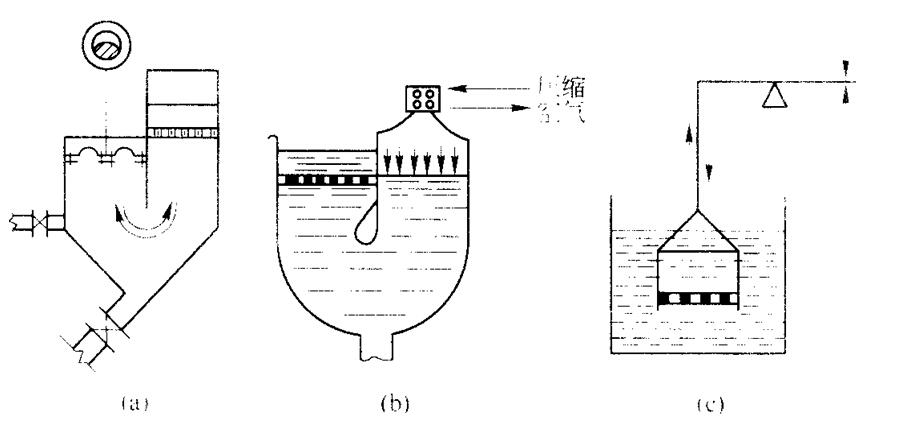
\includegraphics[scale=0.6]{19}
\caption{跳钛选矿图1}
\end{figure}
   \begin{figure}[!ht]
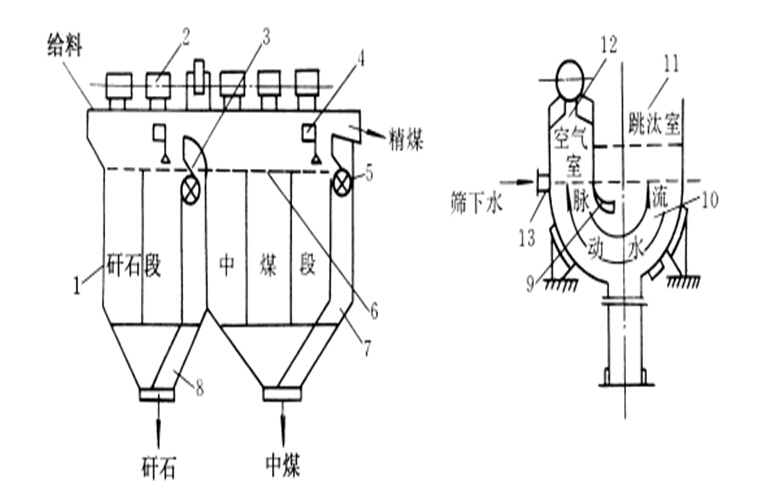
\includegraphics[scale=0.6]{20}
\caption{跳钛选矿图2}
\end{figure}
我国选煤设计研究院在研究跳汰理论、改善末煤及粉煤跳汰分选效果的过程中,研制了多次进气的X系列复合脉动跳汰机,取得了下列效果:①跳汰物料处于松散状态的时间占总脉动周期的比例,由原来的40\%延长到70\%以上,改善了分层状况,增加了有效分选时间;②通过多次进气补充能量,使物料床层达到更好松散状态,可有效控制因吸啜而产生的透筛损失,并降低了耗水量;③降低了分选下限(最低可达0.125mm),加大了分选的粒度范围;④提高了脱硫效果。\par
近年来,动筛跳汰机作为一种块煤分选设备,以其处理量大、用水量少、工艺系统简单、分选效率高、运营费用低等优点,备受选煤界的关注。
\subsection{重介选煤方面}
\begin{center}

   \begin{figure}[!ht]
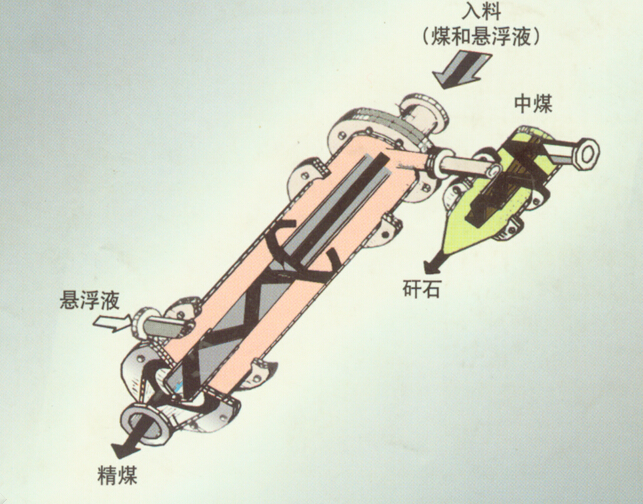
\includegraphics[scale=0.6]{21}
\caption{重介质选矿图1}
\end{figure}

\end{center}
国际普遍采用的重介质选煤技术存在着一些缺点,如原煤入选前需要脱泥和分级,且单机只能出两种产品,而通常要求除了纯精煤和纯矸石外还必须生产中煤,需要两套设备和系统才能满足需要。由于上述原因造成了工艺系统复杂,使投资和加工成本较高。研究如何既能保持重介质选煤的优势又能降低投资和加工成本是世界各国选煤界的热点、难点和努力方向。中国研制的三产品重介质旋流器是目前国际上首次应用于工业生产的、规格最大、技术指标最先进的无压给料三产品重介质旋流器。\par
在重介质旋流器生产过程自动控制方面,由于自动化测控仪表及计算机技术的广泛应用,已实现了悬浮液入口压力变频控制,悬浮液密度、磁性物含量、料液位的自动测控和产品灰分智能控制及技术经济指标的优化控制,提高了设备的处理能力、稳定了产品质量,增强了市场竞争力。目前国际上较为先进的重介质选煤过程自动测控系统属美国PID公司研制的“53SU1000”型重介质选煤过程自动测控系统,其控制算法仍采用PID控制。我国重介质悬浮液密度自校正控制方法和技术比传统的PID方法更精确,将重介质悬浮液密度控制精度稳定在±0.006kg/L,与国外的±0.01kg/L相比,精度提高了40\%。采用精煤灰分仿人工智能控制方法,能实现精煤灰分在线回控。尚未发现国外的重介质选煤过程自动测控系统具备此功能的报道。\par
通过基础研究,完善重介质旋流器分选工艺及设备结构受到许多学者的极大关注。尤其对重介质旋流器内的液相流、颗粒分选规律及其模型化、介质流变学的研究,取得不少成果。如采用不同的入料口结构、加长筒体部分长度等,改善旋流器的分选效果。\par
为改善细粒级煤的分选效果,促使人们重视发展煤泥重介质旋流器分选工艺及设备。过去一般采用小直径(150mm)旋流器、较高入料压力(150kPa)和微细磁铁矿介质(-10μm占50\%)进行分选。实践证明,其操作难度大、介质回收困难。目前研究的方向是采用低压给料和市场可得到的介质实现细粒级煤的精确分选。\par
微细磁铁矿粉重介质旋流器工艺是美国能源部匹兹堡能源中心20世纪80年代末开发的,该工艺目前存在的主要问题是介质的回收、粒度和稳定性问题。Custom煤炭总公司的初步试验表明,采用微细磁铁矿粉重介质旋流器工艺可以有效地处理0.105-0.025mm级粉煤,但介质回收问题尚未根本解决。\par
唐山分院的科研人员较详细地研究了工业生产中使用大直径(Φ≥500mm)重介质旋流器分选不脱泥原煤时,其中的细粒煤的分选效果明显变差的问题。理论研究结果表明,要使细粒级物料在重介质旋流器中得到有效的分选,首要的问题是使细粒级矿粒在旋流器内获得相应高的离心系数。而矿粒在旋流器中所受到的离心力与旋流器直径成反比,因而对细粒级分选宜采用小直径重介质旋流器,并适当增加入料压力,以获得比大直径旋流器较高的离心系数,强化作用于矿粒上的离心力和有效分离速度。同时要改善分选悬浮液的流变特性,采用微细介质以保持悬浮液的稳定性。生产实践证明,采用微细介质小直径重介旋流器分选细粒煤,可使有效分选下限达到0.045mm,且Ep值在0.06-0.08左右,0.5-0.045mm级无机硫脱除率可达65\%以上。\par
    为了提高重介质选煤系统可靠性,人们重视开展耐磨材料的研究,并取得了一定成果。选煤厂材料磨损的类型,即有磨粒磨损、粘附磨损、侵蚀磨损、接触疲劳磨损、磨蚀磨损、微动磨损、高温及高速磨损、塑性变形等。在选煤厂,以上几种磨损类型或单独或几种同时存在于不同使用场合。田庄选煤厂使用耐磨材料结果表明:不锈钢溜槽比普通碳素钢的寿命可延长2-3倍;用特种合金钢整体铸造的重介质旋流器使用寿命可提高2倍以上;特种合金钢铸管使用寿命为碳素钢管的3-5倍。西曲选煤厂使用耐磨陶瓷复合管,其使用周期为普通钢管的13.1倍。
\subsection{浮游选煤方面}

   \begin{figure}[!ht]
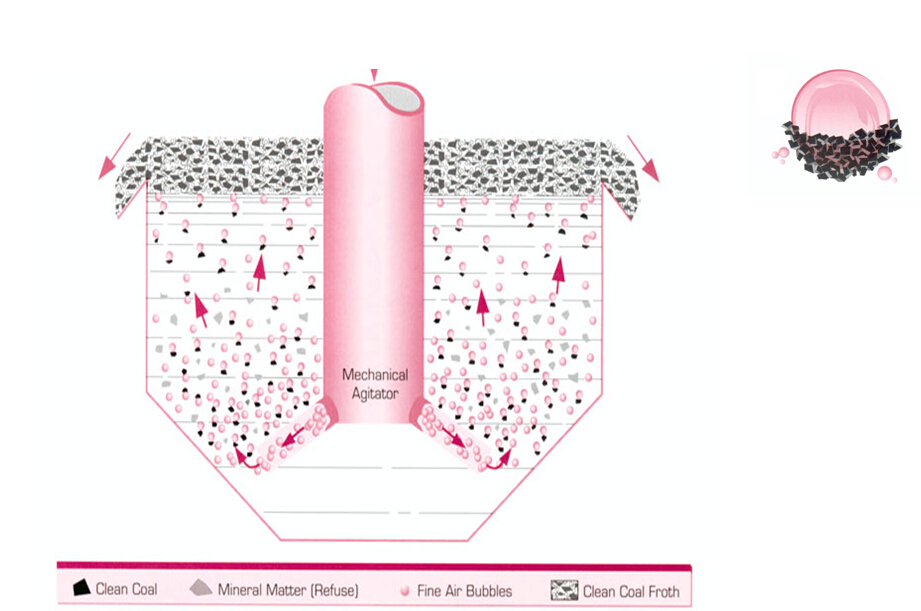
\includegraphics[scale=0.6]{23}
\caption{浮游选煤方面}
\end{figure}
微细煤泥浮选及提高煤泥浮选选择性,始终是国内外研究的技术难点和重点。\par
    在研究提高极细煤泥浮选效果的同时,在国际上还进行了提高浮选粒度上限以简化工艺流程的研究。美国R-Yoon等应用新开发的药剂对韩国的无烟煤煤样进行了实验室试验,可成功地分选上限为2-3mm的煤炭。并对1.41-0mm煤泥进行了半工业性试验,取得了很好结果。 \par
 在浮选设备研制方面特别应该提到的是,为了强化细粒级煤的浮选效果,继20世纪60年代以后,浮选柱再次成为研究热点。在工业上当采用冲洗水喷淋泡沫时,浮选柱的精煤灰分可比机械搅拌式降低1-2个百分点。中国开发的主要为FCMC型旋流——静态微泡式和FXZ型浮选柱,目前在工业上应用的主要是旋流—静态微泡浮选柱和静态浮选柱。 \par
    当前各国对浮选柱研究的侧重点主要是柱体高度和气泡发生器。大量研究工作表明,浮选柱总的发展趋势是气泡发生器由内部充气型向外部充气型发展,柱体由高柱型向低柱型发展。
    \subsection{干法选煤方面}
干法选煤由于不用水、工艺系统简单、投资省、建设周期短、运行费用低和粉尘污染问题已得到解决,近年来在研究和应用方面又有上升的趋势。中国由于西部大开发战略的实施,西部又处于高寒、缺水地区,因此干法选煤技术的应用得到迅速推广。FX型风选机在继续扩大应用范围。今后的发展方向是提高设备的可靠性,并继续向大型化方向发展。
    \subsection{辅助工艺及设备方面}
    \subsubsection{分级破碎设备}
分级破碎机的出现,使选煤厂原煤准备系统的简化成为可能。其特点是集破碎和筛分于一体,能严格控制碎后产品的粒度,过粉碎率低,可省去传统的用预先筛分构成的系统,因而大大简化了工艺环节。\par
    我国煤炭科学研究总院唐山分院吸取国内外各种破碎筛分机的特点,也研发成功系列破碎筛分机,并已推广应用,但规格型号较小,处理能力一般≤300t/h,目前正向大型化方向发展。
\subsubsection{筛分设备}
国内外在筛分设备的研究方面,除了提高可靠性外,其发展的趋势是规格大型化、品种多样化和制造材料多元化。在大型化方面,国外已生产出面积为40-50$m^2$的大型筛分机;在品种上,应用机械振动力、离心力、电磁振动力设计成功多种振动筛分机;在制造材料方面,采用了复合材料、塑料及橡胶等。中国学者对筛机也进行了不少的研究工作。如圆运动梯流棒条筛的研究、复频振动筛的研究、离心振动筛的研究、弹性振杆筛的研究,以及难筛物料堵塞筛孔原因和防堵措施的研究等,取得了不少成果,对推动中国煤用筛分技术的进步发挥了重要作用。
\subsubsection{煤泥水处理}
煤泥水处理是选煤厂生产过程中关键的辅助环节,国内外学者为提高煤泥沉降、回收和洗水澄清效果开展了有针对性的研究工作。 \par
    为强化煤泥水的浓缩、回收,通过试验证明,经磁处理后,煤泥水中悬浮颗粒的沉降速度增加,澄清水的清洁度提高,其固体含量可降低至0.1g/L。通过试验表明,磁处理可降低物料表面电位,改变浆体中的粒度组成,使固体颗粒总的表面积减少,粒径增大,改善物料的过滤性能,提高脱水效率。\par
    为了充分回收、利用煤泥压滤机滤饼,唐山分院研制成功集滤饼定量破碎、穿流干燥作业于一体的煤泥滤饼碎干工艺与设备。生产实践表明,碎干产品水分13\%,粒度<13mm×25mm,可满足商品动力煤的质量要求,已在一些选煤厂推广应用。
\subsubsection{细粒级煤的分选和脱水技术成为研究开发的重点}
对于细粒级煤的分选,除了开发各式浮选柱、高选择性浮选机和微细介质重介质旋流器外,许多学者正注重研究运用综合力场来进行分选。\par
    英国研究在摇床上施加离心力形成为“MGS”’多重力分选机,美国研制了INDECD离心跳汰机,英国研制了PYRADYNE离心跳汰机,德国研制了干选离心跳汰机,澳大利亚研制了较为有名的、可有效分选0.063-0.038mm煤的Kelsey离心跳汰机。\par
    目前在国内外还开展了全氯乙烯(PCE)分选煤泥、粉煤静电选、高梯度磁选、选择性絮凝以及水基磁流体分选技术的试验研究,均尚处于实验室试验阶段。
总的看来,重力与离心力结合对细粒煤进行分选,由于其分选效率高、处理能力大,将具有很好的发展前景。  \par
    在细粒煤的脱水回收方面,取得的最大成果是研制成功和推广应用加压过滤机、超高速离心机和强气压穿流式隔膜挤压压滤机,很大程度上降低了浮选精煤水分,改善了煤泥水处理系统的工况。为了进一步降低细粒煤产品的水分,一些学者建议开展将压滤脱水与热力干燥构成一体的蒸汽压滤脱水技术的研究,预期将具有节能和简化工艺系统等技术特点。
\subsubsection{模块化成为选煤厂设计和建设的新模式}
模块式选煤厂又称装配式选煤厂,由于其系统单机化、工艺简化、布置紧凑化和设备成套化,与传统选煤厂相比,显示出建设周期短、运行成本低和投资效益好的特点,因而近年来在国内外都得到推广。
\subsubsection{选煤生产过程自动控制和全厂自动化水平不断提高}
 由于选煤厂用检测仪表的发展,国外大多数选煤厂实现了高度自动化。在中国,近年来选煤厂自动化技术也取得可喜的进步,研发了一批适应选煤厂生产、管理需求的软、硬件。
 \section{脱硫技术}
 \subsection{重选脱硫}
     重力脱硫法是目前广泛采用的一种脱硫方法,在常用的重力脱硫设备中,较为新型的设备是圆筒形无压给料三产品旋流器,常用的脱硫设备和脱硫率见表2-1。
   \begin{figure}[!ht]
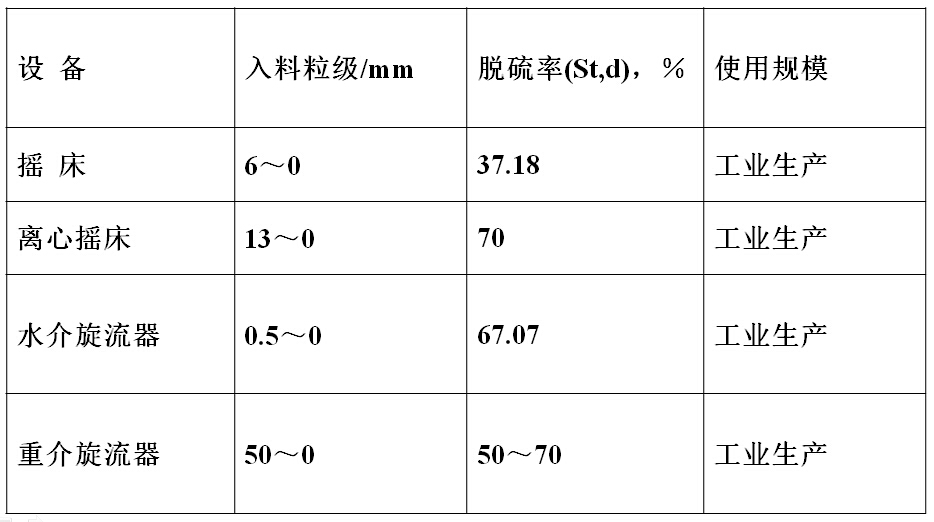
\includegraphics[scale=0.646]{24}
\caption{重力脱硫设备2-1}
\end{figure}
 \subsection{电磁选}
干法摩擦电选技术:用于细粒煤的脱硫降灰。利用充分分散的细粒群在强气体的夹带下,经与摩擦器碰撞,以及颗粒间的碰撞,从而使煤中的有机质和矿物质分别带上极性相反的电荷,有机质颗粒带正电,矿物质颗粒带负电。将不同电荷的有机质和矿物质颗粒群引入高压电场中,吸附到极性相反的极性上。从而实现两者的分离。
煤的磁选脱硫技术:利用煤中黄铁矿有弱磁性和有机质的非磁性差异在强磁场中将黄铁矿从煤中分离;分为煤的湿式高梯度磁选和干式高梯度磁选。有较好的脱硫效果,无机硫脱除60\%以上,但降灰效果不理想,生产成本高,难以推广。

  \subsection{化学脱硫}
  化学脱硫技术主要是利用强碱、强酸和强氧化剂通过化学还原、氮抽提、热解等步骤来完成煤中硫的脱除,常用的有氧化法、熔融法等,通过化学方法脱硫尽管可以脱去煤中几乎所有的无机硫和许多有机硫,但存在工艺条件复杂,成本高等问题。
   \subsection{生物脱硫技术}
   微生物脱硫的原理是利用某些嗜酸耐热菌在生长过程中消化吸收Fe$^{3+}$,S0等特性,从而促进黄铁矿氧化分解与脱除,硫的脱除率在90\%以上。主要有堆浸法、表面氧化法、浸出法等方法。但脱硫反应时间长,微生物繁殖慢,并有酸性处理液产生,形成二次污染,难以适应工业化脱硫的需要,至今未达到实用阶段。
   \subsection{微生物表面处理浮选法}
利用亲水性的细菌微生物,如氧化硫杆菌或氧化亚铁杆菌等。利用它们对黄铁矿的选择性吸附和大量吸附后对黄铁矿表面的活性作用-增加亲水性,使得黄铁矿被抑制,通过浮选尾矿排除。与传统的微生浸出脱硫法不同,主要是通过细菌在矿浆中对黄铁矿的快速吸附,而改变黄铁矿表面性质。存在的问题仍然是多数细菌生长和左右作用都是在酸性条件下,且细菌生长较慢。目前正致力于发现和培育能在中性条件下快速生长和改性的微生物。
 \subsection{煤泥脱硫技术}
 常用的方法有选择性絮凝,油团聚技术等方法。\par
   选择性絮凝根据可燃体与非可燃体两部分颗粒表面性质的不同进行分选。是一种较为理想的极细粒煤泥分选方法。该方法可以脱除煤泥中单体解离的微细粒黄铁矿,从而降低煤泥中黄铁矿硫的含量。\par
   油团聚法是将选择性絮凝与重液旋流分选技术合二为一,可以得较好得降灰和脱硫效果,但生产成本比正常得选煤成本高得多,且处理量远低与选煤厂中的煤泥处理量,目前还没有应用到工业生产中。



  \subsection{其他脱硫}
旋流水膜脱硫、超音波脱硫、螺旋分选机脱硫和热解脱硫技术等。
\section{动力配煤}
\subsection{动力配煤的意义}
根据工业锅炉对煤质的特定要求, 将几种不同性质的单种煤, 按一定比例进行配合而得到一种对锅炉燃烧最有利的燃料煤, 就称为动力配煤。\par
    目前, 我国的工业锅炉数量已达40~50万台, 蒸发量约 80~100万吨, 年耗煤量达3~4 亿吨, 约占全国煤炭消耗总量的 1/3 左右, 这些锅炉平均运行热效率只为 60\%-65\%, 其中占工业锅炉总量的 40\% 小型锅炉有不少热效率还达不到 60\%, 每年浪费煤炭约 3000 多万吨。 \par
    从 70年代末到 80 年代初 , 上海、天津等一些工业锅炉比较集中的大城市就曾采用好煤次煤搭配或不同性质煤炭混合 , 向用户供应质量相对稳定的煤炭 , 这种初步的配煤办法 , 很受用户欢迎。到 90 年代全国已建成动力配煤生产线 200 余条 , 年配煤量已达000~3000 万吨 , 其中以天津、上海、北京等大城市比较集中, 这些大城市年配煤量已近 1000 万吨。
    \subsection{动力配煤的主要优点}
 煤炭作为燃料使用, 一般都应按照就地取材, 就近使用的方针, 充分利用当地的煤炭资源 , 特别是一些低质煤和小窑煤都要充分利用, 但这些煤往往因为质量较差和质量不稳定, 造成使用困难, 也使锅炉热效率大大降低, 采用动力配煤可以使用户得到质量稳定的煤炭, 即使煤炭质量差些, 如能保证煤质稳定, 用户也可通过改造锅炉和提高司炉工人的操作技术, 掌握燃用一定质量煤炭的最佳条件, 使质量较差的煤也能充分发挥其作用, 使煤的利用效率和锅炉热效率得到提高。另外, 在进行配煤时还可使煤中块末分开, 将块煤以较高价格供给需用块煤的用户以提高经济效益, 这样即可实现煤炭的就近使用, 节约运力, 物尽其用, 使煤炭得到合理的利用。
 \subsection{工业锅炉对煤质的要求}
   现代工业锅炉燃烧方式各异, 设计制造差别甚大, 不同的燃烧方式对煤质也有不同的技术要求。锅炉燃烧方式主要分为层状燃烧、室式悬浮燃烧和沸腾燃烧三大类。
\subsubsection{室式悬浮燃烧}
  室式悬浮燃烧是指燃料在无炉排的火室内悬浮燃烧方式, 要求煤粉磨在很细 (20-50 μm), 对煤质要求不太严格 , 这类锅炉需煤量大, 炉型设计针对性强, 燃煤多是定点供应 , 一般不需采用动力配煤。
\subsubsection{沸腾燃烧}
沸腾燃烧是将燃料布置在布风板( 即流化床 )上 , 由强风吹到沸腾状态下的燃烧方式。这种燃烧方式主要用于燃用低质煤,但要破碎到 8mm 以下才能使用, 一般也不需采用动力配煤。
\subsubsection{层状燃烧}
层状燃烧是指燃料在炉排上以固定不动或沿炉排表面移动,但不离开炉排,空气通过炉排与燃料接触进行燃烧的方式。动力配煤主要是针 对这种燃烧方式的锅炉。  \par
现仅就采用层燃方式的工业锅炉对煤质的要求及煤质对锅炉燃烧及运行的影响简述于下 :
\subparagraph{水分}  一般认为, 煤的外在水分应根据煤的粉末含量而定, 如煤粉过多, 外加水量就应多些, 当 <6mm 的煤粉含量在 20\%-40\% 时, 添加外水量以 6\%-8\% 为宜。
\subparagraph{灰分} 由于灰分在煤燃烧时因分解吸热使煤难于着火和使炉温降低, 灰分在煤燃烧中还能形成灰壳, 使煤难以燃尽 , 因此燃用高灰分煤, 锅炉热效率普遍降低。如对燃用发热量较高的烟煤时, 灰分与锅炉热效率相关的经验公式为 :
$$\eta =80+0.17A_{ar}-0.017(A_{ar})^2 $$
\begin{center}
	式中η一锅炉热效率,\%;\\
	Aar一燃煤收到基灰分,\%
\end{center}
\subparagraph{挥发分}
挥发分是评价动力用煤的重要指标。工业锅炉一般要求煤的挥发分要高一些, 煤的干燥无灰基挥发分以 20\%-30\% 较好。
\subparagraph{发热量}
发热量高的煤不一定热能利用率就高 , 它还必须与锅炉的炉型相适应 , 才能提高锅炉的热效率以充分利用煤的热能。一般工业锅炉使用的煤炭, 其发热量以 14.63-23.OOMJ/kg (3500- 550Okcal/kg) 较为合适.
\subparagraph{灰熔点}
当工业锅炉炉膛温度达到或超过灰渣的软化温 度 (ST) 时 , 煤炭即会结成渣块 , 影响通风和排渣 , 造成局部高温、恶化传热, 使灰渣含碳量增高, 影响锅炉正常运行。层燃锅炉炉膛温度一般在 1350 ℃左右 , 通常只要煤炭熔点达到 1250 ℃以上 , 煤灰就不会结渣。
\subparagraph{硫分}
动力配煤中要求煤的硫分越低越好, 一般应控制在2\%以下, 个别高硫煤地区不应超过3\%。
\subparagraph{结焦性或粘结性} 一般可用煤的挥发分测定中的焦渣特征 (1-8 级 ) 来表示煤的粘结性, 以焦渣特征为 2-5 级为宜。
\subparagraph{粒度}  入炉煤的最大粒度不宜超过 30mm, 小于6mm 的碎煤不超过30\%, 小于0.2mm 的煤粉不超过2.5\%, 一般层燃锅炉以烧用 <25mm 的混未煤即可。
\subsection{动力配煤的优化配置}
动力配煤应遵循以下原则 :
\subsubsection{动力配煤的原则}
\begin{itemize}
\item 生产的配煤必须满足工业锅炉的基本要求使煤质与锅炉特点相适应, 并能保证配煤质量有相对的稳定性
\item 配煤要有利于提高锅炉热效率, 保证锅炉的正常出力,以节约煤炭
\item 本着节约优质煤的原则, 在配煤中要尽量扩大低质煤的比例, 做到物尽其用
\item 要注意延长锅炉寿命和保护环境, 配煤中的硫分要控制合适的界限
\item 要充分考虑尽量缩短煤炭运输距离, 就近找煤 , 以缓解运输紧张局面
\item  配煤品种要尽可能地少些, 以简化配煤工艺, 降低配煤成本
\end{itemize}
\subsubsection{. 动力配煤的优化设计}
动力配煤的优化设计的原则是在一定约束条件下追求目标函 数的极值, 具体分为四个步骤 : 即确定约束条件 , 确定目标函 数 , 建立数学模型和解出最优配方。
\subparagraph{确定约束条件} 工业锅炉对煤质的各种指标都有特定的技术要求 , 这就是动力配煤的基本约束条件。
\subparagraph{确定目标函数} 目标函数的确定是依据实际情况 , 针对所要达到的目标而确定,在动力配煤中应追求的目标主要有以下三方面 :
\begin{itemize}
\item 追求成本最低
\item 追求优质煤配比最小
\item 追求低质煤配比最大
\end{itemize}
\subparagraph{建立数学模型}
根据上述的约束条件和目标函数, 可建立动力配煤优化配方的数学模型。
\subparagraph{解出优化配方} 优化配方就是使配成的新品种煤的各项技术指标能符合锅炉设计制造的要求, 在这基础上再追求配煤的最低成本, 以达到配煤的最佳效果。
\subsection{动力配煤的固硫技术}
\subsubsection{国内外燃煤脱(固)硫技术现状} 燃煤脱(固)硫技术可分为三大类:①燃烧前脱硫,如选煤等;②燃烧中脱(固)硫,如工业型煤固硫、动力配煤加固硫剂固硫、炉内喷钙、循环流化床固硫等;③燃烧后脱硫,即烟气脱硫。
\subparagraph{燃烧前脱硫}  该方法可分为物理法、化学法及生物法三大类。
\subparagraph{燃烧后脱硫(FGD)}
   FGD技术主要是利用吸收剂或吸附剂去除烟气中的SO$_2$,并使其转化为较稳定的硫的化合物或单体硫。
 \subparagraph{燃烧中脱硫}
该技术使在煤中添加一定的固硫剂,将煤在燃烧气化时生成的气态硫氧化物在炉内吸收,气相中残存的硫氧化物与刚进入炉内的脱硫剂接触而被吸收,这样排出的气体中二氧化硫含量就大大降低了。这种方法可大大减少燃烧后脱硫设备,但固硫剂部分或全部参与燃烧过程,将会影响煤的燃烧性能。此外,固硫剂中的碱性物质等的利用率低,以及形成的硫酸盐的再分解等,导致脱硫效果下降。目前,使用最普遍的是以石灰、石灰石、方解石、白云石等为主的钙系固硫剂。
\subsubsection{固硫剂及其助剂的研制开发}
凡能与煤在燃烧过程中生成SO$_2$或SO$_3$起化学反应或物理吸附形成固态残渣而留在煤灰中的物质均可作为固硫剂。\par
    目前使用最多、价廉易得得仍是碳酸钙、氢氧化钙等,俗称钙基固硫剂。普通的钙基固硫剂具有钙的利用率低、高温固硫效果差的不足。因此,为了提高固硫率,在制备固硫剂的过程中往往添加一定量的助剂来改善其表面性质,以提高固硫率;或者将固硫剂进行活化改造,以利于提高固硫的利用率与固硫率。
 \subparagraph{固硫技术的基本原理}
  a煤中硫的赋存状态及其在燃烧过程中SO$_2$的析出特征
燃煤中硫形态可分为有机硫和无机硫两大类。有机硫在煤加热到400℃时开始发生分解,但不同煤化程度的煤稍有差异.
$$\mbox{有机硫}+O_2\longrightarrow SO_2 ······$$

黄铁矿硫在300℃时开始失去硫分,形成磁硫铁矿Fe$^{1-x}S$
   (0<x<1)和赤铁矿Fe$_2$O$_3$,但FeS2大量分解则是在650℃以上,其分解产物与气氛有关.由黄铁矿形成SO2过程可写成如下分步方程:

\begin{eqnarray}
\begin{split}
           4FeS_2+11O_2→2Fe_2O_3+8SO_2↑\\
  7FeS_2+6O_2→Fe_2O_7+6SO_8↑\\
  3Fe_7S_8+38O_2→7Fe_3O_4+24SO_2↑\\
  R-S_x+nO_2→nCO+xSO_2↑+mH_2O\\
  \end{split}
\end{eqnarray}
一般来说,硫酸盐中的硫难于分解出来,为不可燃硫,进入灰分中。但在高温下有些金属盐是可以分解的。如:

\begin{eqnarray}
\begin{split}
  CaSO_4+CO→CaO+CO_2+SO_2↑\\
 2CaSO_4→2CaO+O_2↑+2SO_2↑
  \end{split}
 \end{eqnarray}
 \subparagraph{固硫剂的固硫反应}
燃烧过程中最常用的固硫剂是钙基固硫剂和在钙基固硫剂中掺加一定比例的含金属或金属氧化物的工业废料的添加剂。如石灰石(CaCO$_3$),电石渣(Ca(OH)$_2$)、白云石(CaCO$_3$、MgCO$_3$)和含铁废料、含锌废料、含钠盐废料等。其反应如下:
石灰石反应式
\begin{eqnarray}
\begin{split}
  CaCO_3→CaO+CO_2 \\
  CaCO_3+SO_3→CaSO_4+CO_2 \\
  CaO+SO_2→CaSO_3 \\
  CaSO_3+\dfrac{1}{2} O2→CaSO_4 \\
  CaO+SO_2+\dfrac{1}{2} O2→CaSO_4 \\
   \end{split}
\end{eqnarray}
电石渣硫化反应式
\begin{eqnarray}
 Ca(OH)_2+SO_2+\dfrac{1}{2} O_2→CaSO_4+H_2O
\end{eqnarray}
白云石反应式
\begin{equation}
\begin{split}
CaCO_3·MgCO_3→CaO·MgO+CO_2\\
  CaO·MgO→CaO+MgO
\end{split}
\end{equation}
MgO与SO2反应速度很低,可忽略。CaO在有富余氧气时与SO2发生如下硫酸盐化学反应:
\begin{equation}
\begin{split}
  CaO+SO_2+\dfrac{1}{2} O_2→CaSO_4   \\    CaO+SO_3→CaSO_4
\end{split}
\end{equation}
其他金属氧化物与SO2发生硫酸盐化学反应式
\begin{equation}
\begin{split}
  MO+SO_3→MSO_4     \\     MO+SO_2+\dfrac{1}{2} O_2→MSO_4
\end{split}
\end{equation}
固硫产物的再分解
\begin{equation}
\begin{split}
  MSO_x→MO+SO_2
\end{split}
\end{equation}
\subparagraph{提高钙基固硫剂高温固硫效果的途径分析}
一般认为钙基固硫剂高温固硫效果差,主要原因:\par
①煤中硫在燃烧过程中的析出规律各不相同;
②高温下CaSO$_4$稳定性下降,易分解成CaO和SO$_3$;
③高温下固硫剂表面烧结失活,比表面积减小;
④高温下煤中硫的分解速度大于CaCO$_3$的分解速度,使含硫气体未来得及与固硫剂发生反应而排出;
⑤实际固硫反应中,含硫气体首先在固硫剂表面发生固硫反应,使固硫剂表面及内孔被CaSO$_4$覆盖或堵塞,从而影响固硫效果。\par
从以上分析可知,提高钙基固硫剂高温固硫效果的关键:\par
①在固硫剂中添加具有促进作用的化合物,使之在固硫过程中形成高温下稳定的固硫产物。如硫酸盐的络合物等,减少固硫产物在高温下分解;
    ②采用多种化合复合型添加剂捕捉煤中不同化合成分的硫;
    ③利用促进剂改善固硫剂的微观结构,提高抗烧结能力;
    ④降低固硫剂开始分解温度,从而改善固硫剂捕捉在550℃以下分解的低温硫能力;
    ⑤固硫剂固硫能力应与煤种,尤其是硫含量、硫成分及煤中灰分、产率及成分相适应。
    \subparagraph{影响动力配煤固硫效果的因素}
    \begin{itemize}


\item    Ca/S摩尔比的影响:
\item   固硫剂粒度的影响
\item  燃烧温度对固硫率的影响
\item  燃烧工况的影响
\item  添加方式的影响
\item  固硫剂与煤种的适应性

   \end{itemize}
 \subparagraph{几种固硫剂的基本配方及其固硫率}
 HZ系列节能清洁燃烧剂:是以矿物质、生物质、碱金属促进剂为基本部分,再加入具有催化燃烧的含金属盐或金属氧化物工业废料与钙基固硫剂按一定比例配合而制成,形成既可直接在燃烧过程中固硫,又有一定催化作用。\par
 ZD系列洁净燃烧添加剂:
  与HZ系列的组成成分和作用基本相同,在加入相当于煤中硫含量4.13-7.21倍时,其固硫率约38\%-41\%。\par
  HN固硫剂:
  主要成分CaCO3,在固硫剂加入量为煤中硫含量的2.75-3.88倍时,固硫率为41\%。固硫剂粒度越细,固硫效果越好,加大用量无明显固硫效果。\par
MY941和MY942型烟煤添加剂:主要成分CaO、Al$_2$O$_3$、Fe$_2$O$_3$、MgO等工业废弃物及氧化剂。其中MY941为液体添加剂可溶于水中使用,加入量为0.8\%,MY942为固体添加剂,于煤掺混后使用,对含硫1.9\%的煤,加入量为3\%,用MY941固硫率为6.7\%,加入MY942固硫率为10.39\%。\par
MHS系列添加剂:
由Al$_2$O$_3$、SiO$_2$、Fe$_2$O$_3$、CaO、MgO等金属氧化物和适当的助燃剂组成,与钙基固硫剂配合使用,加入量约为煤样量0.5\%-1.5\%,其作用一是加快低温时析出的SO$_2$与钙基固硫剂的固硫反应,提高固硫剂利用率和固硫反应速度;二是在高温下生成含硫的金属复合物,改变固硫产物的结构形态,阻止CaSO$_4$的分解。
\chapter{型煤}
本章主要讲述型煤的概念、种类;型煤粘结剂;民用型煤和工业型煤在我国的应用情况及特点。\par
要求掌握型煤常用的粘结剂;熟悉型煤的工艺;了解型煤的分类。
\section{型煤种类}
型煤是用机械方法 ,将粉煤制成具有一定强度和形状的煤制品。型煤按用途可分为两大类:民用型煤和工业型煤。\par
    蜂窝煤是民用型煤的主要品种。普通蜂窝煤以无烟煤为原料,上点火蜂窝煤以烟煤、褐煤、煤泥、劣质煤等多种资源为主要原料添加各种易燃物质加工而成。\par
    工业型煤的形状有椭球形、笼形、中凹形、枕形、马赛克形、圆柱形、砖形等;按成型方式可分为辐压、冲压、挤压、圆盘造粒型煤; 按生产工艺可分为冷压、热压成型、高压、低压成型及有无粘结剂成型。我国普遍采用加粘结剂、冷态、低压条件下辊压成型工艺 , 工业型煤大多为椭球形。\par
    \section{型煤粘结剂}
    不同用途的型煤对粘结剂有一定的要求,型煤粘结剂通常应具备如下条件:
    \begin{itemize}
 \item   粘结能力强、流动性好、在煤粒表面易扩散、分布均匀;
  \item  能很好润湿煤表面也且增加粒子间的作用力;
  \item  来源广、价廉、无污染;
  \item  无机物含量低、尽量少增加型煤灰分、固硫效果好;
 \item  制备工艺简单;
  \item  使型煤具有抗湿防水性能。

    \end{itemize}
   国内外研究开发和应用的粘结剂达几百种, 根据其基本性质可分为四大类。
 \subparagraph{有机粘结剂} 焦油、沥青、淀粉、腐植酸、本质素磺酸盐、聚乙烯醇、聚醋酸乙烯、聚氨酶等。
 \subparagraph{无机粘结剂 } : 粘土、膨润土、高岭土、石灰、水玻璃、石膏、水泥、氯化纳等。
 \subparagraph{工业废物粘结剂} 纸浆废液、制糖废液、制革废液、酿酒废液、糠隆渣、电石渣、血浆、生化污泥等。
 \subparagraph{复合粘结剂 } : 粘土一纸浆废液、淀粉一膨润土、麦秸一石灰等上述2种或3种粘结剂的复合物。\par
粘结剂的粘结能力决定型煤的抗碎强度;粘结剂的热性能对型煤的发热量、热态强度、灰熔融性与灰渣强度等有较大影响。\par
    有机粘结剂粘结能力强, 本身具有一定的发热量,可提高型煤的冷态机械强度,对型煤的热性能作用不明显,其优点是不增加型煤灰分;\par
    无机粘结剂粘结能力不如有机粘结剂 , 本身没有发热量 , 但多数无机粘结剂来源广,价格低, 制取的型煤热态强度高。\par
    国内蜂窝煤应用最广的粘结剂是石灰、粘土、煤泥类无机物,可保证足够的灰渣强度。上点火蜂窝煤的易燃层,烧烤炭,火锅炭,手炉煤球等采用淀粉类粘结剂,粘结性能强而无污染。 \par
工业型煤的粘结剂, 许多国家采用煤焦油和沥青, 型煤强度高, 防水性能好, 但来源有限, 价格高, 且生产使用中对环境有污染;石灰碳化煤球早已在小合成氨厂推广应用, 其后腐植酸煤球, 纸浆废液煤球也得到应用。煤科总院北京煤化所开发出了钙系复合粘结剂和有机复合粘结剂等。\par
    国外研究重点是直接从煤中提取粘结剂。国内开发重点是价廉、易得的工农业废弃物,已有多种系列粘结剂用于褐煤、烟煤、无烟煤成型。某些粘结剂生产的型煤还有脱硫和提高反应性的功能。
\section{民用型煤}      我国民用型煤加工已有成熟技术, 蜂窝煤成型机械制造厂已发展到 200 多家。以无烟煤为原料的普通蜂窝煤得到全面推广;以烟煤、褐煤为原料的上点火蜂窝煤消烟技术取得很大进展,已开发出多种粘结剂, 如石灰、煤泥、电石渣、烟道灰等, 改变了传统的黄土粘结剂,且有的粘结剂还可起到固硫作用。\par
    作为我国民用型煤主体的蜂窝煤, 配以先进的炉具, 热效率比烧散煤提高 20\%-45\%, 一般可节煤 20\%-30\%, 烟尘减少 40\%-60\%,CO2减少 80\%;加固硫剂后SO2 减少40\%-60\%, NO$_x$ 减少 55\%,Bap 减少90\%, 烟气黑度达到林格曼 1/4 级。节能、环保效益显著。\par
  我国民用型煤的普及率还很低。目前全国约 85\% 的城镇居民和15\%的农民以原( 块 ) 煤作为生活燃料, 全国居民生活用煤年消耗量在2亿吨以上,目前民用型煤年产量在 7000 万吨以上,型煤普及率为 30\% 强, 发展潜力仍很大。因此必须开发和推广以烟煤、褐煤为原料的上点火蜂窝煤及配套炉具,但需解决成本较高的问题。
  \section{工业型煤}
 \subsection{工业型煤的种类 }
 \begin{itemize}
 \item   造气型煤
\item 锅炉型煤:生产分为集中成型和炉前成型。后者成型工艺简单,通常
无需加粘结剂,不用烘干,使型煤生产成本大幅度降低, 得
到越来越多的用户欢迎。
\item 型焦及炼焦配用型煤
\item 工业型煤市场:我国现有层燃工业锅炉数十万台,工业窑炉 10 余万台,
年耗煤约 4 亿吨,蒸汽机车7千台,年耗煤约 2500 万吨;
小型氮肥厂1306家,制气用无烟煤3500万吨,总计年耗煤约5
亿吨。    \par 固定床气化炉需块状原料, 块煤不足部分由型煤补充。工业锅炉、窑炉、蒸汽机车对原料煤粒度有一定要求, 如直接用原煤散烧会造成严重的粉尘污染和能源浪费。 如能充分利用粉煤资源, 生产型煤用于燃烧, 市场前景相当广阔。
\end{itemize}
\subsection{工业型煤的特点}
工业锅炉与民用炉具有本质上的区别, 一台工业锅炉所消耗的煤量是一台民用炉具燃煤量的几千甚至上万倍。如果还按照民用型煤的制作方式, 由型煤厂生产型煤, 然后分送到各用户, 势必造成型煤制造厂的规模庞大, 一方面需要大量的投资;另一方面需要大量的粘结剂以保证在运输过程中型煤不大量破碎。\par
    过去在工业型煤试制过程中曾经采用过的粘结剂有两大类:一类是憎水性粘结剂, 如各种沥青, 气化焦油, 焦油渣等;另一类是亲水性粘结剂, 如纸浆废液, 腐植酸盐, 糠醒渣废液, 电石渣和粘土等。\par
由于型煤制作量和制作成本的关系, 制作民用型煤大都用粘土作为粘结剂, 但作为工业锅炉燃用的型煤, 如果也采用粘土作为粘结剂就会出现增加型煤的灰分、运输量增大、锅炉热效率降低、成本有所增加的弊病;而采用其它种类的粘结剂 , 也存在着可利用的数量有限, 或者加工成本提高较大造成节能不节钱而不受用户欢迎的被动局面。因此, 要使工业锅炉能普遍使用型煤, 节约能源, 就必须完全抛弃原有型煤的制作模式, 采用无粘结剂, 不经运输, 直接入炉的炉前成型模式, 也叫自成型模式。所谓自成型就是指利用煤本身的水份,经过挤压成型而不需要任何粘结剂的一种强度较低的型煤制作工艺, 其型煤的成型力主要是依靠毛细水分的粘附力和不规则煤粒之间的相互联结。
\subsection{工业型煤的应用}
型煤在工业锅炉中试验和应用的情况表明:工业锅炉燃用型煤有如下的优点:
\begin{itemize}
\item 型煤尺寸均一, 孔隙率高, 能强化燃烧, 灰渣含碳量明显减少。
\item 型煤有较好的热变形特性, 确保型煤能完全烧透。
\item  型煤燃烧时, 飞灰和漏煤量大为减少, 能消烟除尘, 减轻污染人节约能源。
\item 型煤可以有较合适的焦渣特性 , 以满足层燃的要求。
\item 型煤可以获得较高的灰熔融性。
\item 使用型煤可以降低炉内空气过剩系数, 减少床层通风阻力, 降低风机功耗, 减少排烟损失, 提高锅炉效率。



 \end{itemize}
型煤如在成型前加入石灰石粉或电石渣等脱硫剂, 还可以降低烟气中SO$_2$的排放量。也可以加入一定量的助燃剂, 有助于在层燃炉中燃用劣质煤。\par
    此外, 自成型型煤不仅仅局限于在工业锅炉中应用, 还可以广泛地适用于层燃方式的各种工业炉窑、蒸汽机车等场合。因此,研究并推广使用自成型型煤是当前工业锅炉,工业炉窑节能的一项重要措施,有十分广阔的前景。
\section{型煤生产工艺}
 目前,普遍使用的粉煤成型方法主要有无粘结剂冷压成型、有粘结剂冷压成型及热压成型三种。
 \subsection{无粘结剂冷压成型}
     即粉煤不加粘结剂,只靠外力作用而成型。许多国家已广泛采用这种方法来制造泥煤、褐煤型煤,作为家庭燃料或工业燃料。对于烟煤和无烟煤,由于煤化度高,其粉煤的无粘结剂成型较为困难。粉煤无粘结剂成型不需要添加任何粘结剂,不但节约大量原材料,相应地保持型煤的碳含量,而且简化成型工艺等,是粉煤成型的一个重要发展方向。
\subsubsection{年轻褐煤无粘结剂成型} 根据煤化度的高低,褐煤可分为3类,其中最为年轻的褐煤结构疏松,容易粉化,刚刚开采出来时的水分含量高达45%以上,热值很低,因而工业价值也低。为充分利用褐煤资源,将其制成型煤,以改善煤质,提高使用价值。年轻褐煤制取燃料型煤的主要工艺流程如下:

    \begin{figure}[!ht]
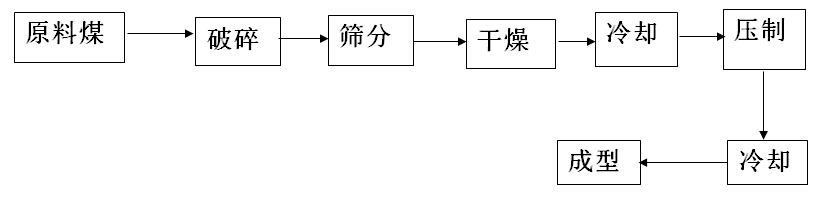
\includegraphics[scale=0.6]{25}
\caption{燃料型煤的主要工艺流程}
\end{figure}

\subsubsection{烟煤无烟煤无粘结剂成型}
烟煤、无烟煤无粘结剂成型被认为是有一定困难的。随着煤化度的增高,煤中的氢含量逐渐减少、碳含量逐渐增加的同时,煤的胶团结构越来越大,排列更加整齐,煤的硬度、弹性越来越高,塑性越来越低。因此,成型性能越来越差。\par
    烟煤、无烟煤无粘结剂成型在克服煤的硬度大、弹性高所造成的成型困难方面主要采用强制高压和改善成型的方式。\par
    使用强制高压方法的实质就是破坏煤粒弹性,消除它对成型的不利影响。由于该方法成型压力高,成型机结构复杂,动力消耗大,材质要求高,生产能力较低,因而生产成本较高,工业上很难广泛采用。\par
    在型煤压制方式上做必要的改进,可以在一定程度上克服煤粒弹性的影响,增加塑性变形,达到成型的目的。粉煤在承受较高压力下,煤粒彼此紧密接触后,使煤粒扭动。煤粒的表面积就会发生适当的剪切变形,这样煤粉内部的“架桥”就会被破坏,内摩擦减小,从而使煤粒进一步接近。同时由于剪切能增加煤粒的塑性变形,这种塑性变形产生于煤粒表面上,这样就有利于粘结。\par
    对于某些质软的烟煤、无烟煤的粉煤无粘结剂成型并不困难,也不需要特殊的成型方式即可直接成型。
\subsubsection{清水湿煤棒}
清水湿煤棒的生产流程图见图。
    \begin{figure}[!ht]
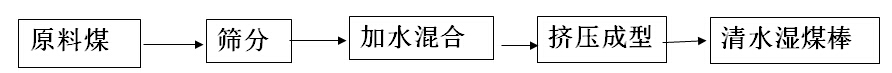
\includegraphics[scale=0.6]{26}
\caption{水湿煤棒的生产流程}
\end{figure}
原料煤经筛分,得到10mm以下的粉煤加水混合均匀,物料水分控制在15\%-18\%范围内,送入螺旋挤压机中挤压成型。\par
煤质较软的煤种或者风化后的煤塑性强,成型后可得到质量较好的清水湿煤棒。

 \subsection{粉煤有粘结剂冷压成型}
尽管有粘结剂成型的工艺流程很多,但这种类型的型煤生产过程必须包括成型原料的制备、成型和生球固结三个程序。其简要的生产流程如下
    \begin{figure}[!ht]
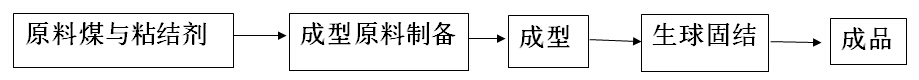
\includegraphics[scale=0.6]{27}
\caption{燃料型煤的主要工艺流程}
\end{figure}
成型原料制备包括干燥、破碎、配料、混合4个主要环节。 \par
采用疏水性有机粘结剂成型时,原料煤的水分含量大于4%时,就不能正常粘结,因此,需把原料煤的水分干燥至4%以下;采用亲水性有机粘结剂或水溶性无机粘结剂时,一般成型水分控制在8\%-10\%之间。一般采用的粒度在0-3mm。\par
    刚从成型机出来的型煤强度很低,不能直接应用,这时型煤里的煤粒暂时被粘结在一起,水分含量较高。为了保证粘结剂能成为骨架,使煤粒之间能牢固地粘结,生球固结就成为不可缺少的一个环节。\par
    采用的粘结剂不同,因而有不同的生球固结方法。以石灰为粘结剂的石灰炭化型煤,生球固结采用碳化方式。以水泥为粘结剂的型煤,生球固结采取养护方式。以亲水性有机物、水溶性无机物以及不溶性无机物为粘结剂的型煤,型煤固结一般采用干燥的方式。
 \subsection{粉煤热压成型}
 煤加热到一定温度时就会发生热解,一般而言,温度在340-500℃时,就有气体和液体产生,同时形成胶质体,煤逐渐软化熔融,但随着加热温度的提高,热分解进一步加剧,软化了的煤便逐渐固化。利用煤在加热过程中产生的胶质体作为粘结剂将煤制成型煤。热压成型工艺按加热的方式可分为气体热载体快速加热热压成型工艺和固体热载体快速加热热压成型工艺两大类。
 \subsubsection{气体热载体快速加热热压成型工艺}
 该工艺主要由煤的干燥预热、快速加热后维持温度以及热压成型3个工序组成。
    \begin{figure}[!ht]
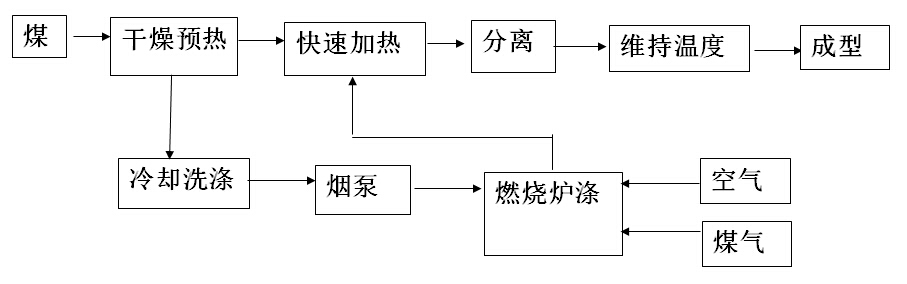
\includegraphics[scale=0.6]{28}
\caption{热压成型3个工序}
\end{figure}
\subsubsection{固体热载体快速加热热压成型工艺}
这种工艺主要由固体热载体加热;烟煤的预热、混合及维持温度;热压成型3个工序组成图1。

    \begin{figure}[!t]
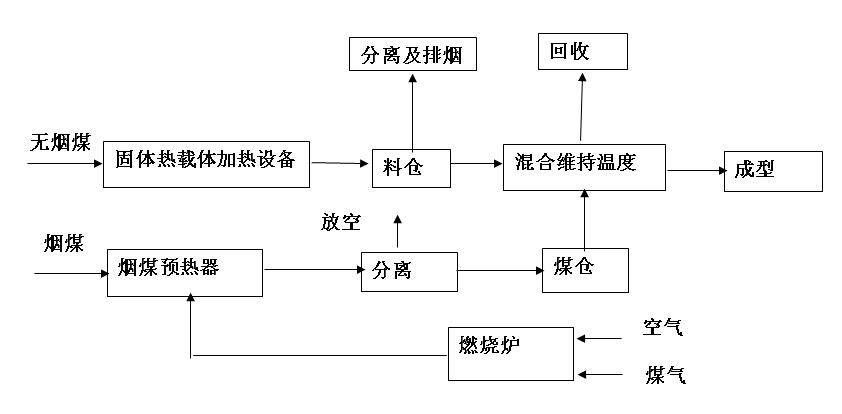
\includegraphics[scale=0.6]{29}
\caption{热压成型3个工序组成图1}
\end{figure}
该工艺特点:由于采用两种煤粉通过在混料机内混合达到快速加热的目的,烟煤热分解的产物可单独回收利用;热效率高;调节加热温度方便。缺点是不能使用单一煤种的热压成型。
\chapter{水煤浆技术}
本章主要讲述水煤浆的概念、产生及发展;煤的成浆性;水煤浆的制浆工艺及添加剂;水煤浆在贵州省的应用。\par
要求掌握煤的成浆性及制备技术;熟悉水煤浆添加剂。了解水煤浆的产生及发展、水煤浆管道输送和水煤浆在贵州的应用。
\section{水煤浆的产生及发展}
\subsection{水煤浆的产生}
水煤浆(CWM)是70年代兴起的以代油为目标的新型燃料,它是把洗选后的低灰分精煤加工研磨成微细煤粉,按煤约70\%,水约30\%的比例和适量(约1.0\%)的化学添加剂配制而成的一种煤水混合物,这种煤水混合物又称水煤浆(CWS)或煤水燃料(CWF) 。由于水煤浆既能保持着煤的物理化学性能,又能象石油一样具有良好的流动性和稳定性,可以泵送,又易储运和调整,可以雾化燃烧,又属低污染洁净燃料,而且燃烧效率高,有着代油、节能、环保、综合利用等多种效益,受到世界各国工业界的高度重视,在不久的将来,水煤浆将会成为煤炭深加工利用诸多技术中最具有竞争力的一项技术。
\subsection{水煤浆在我国的发展}
中国的水煤浆研制始于1982年。1983年1月,国家科委“水煤浆制备与燃烧技术”正式列为国家“六五”攻关项目。1983年5月,中国矿业大学北京研究生部制备的“大同水煤浆”首次在我国浙江大学试烧成功。1984年2月,第二次制备的4吨“抚顺及思口水煤浆”再次试烧成功。1984年8月,中国矿业大学北京研究生部在实验室制备70吨水煤浆在北京造纸厂的20蒸吨/时工业锅炉上代油燃烧成功。进入“七五”后,该项目得到了国家进一步支持,组建了“华煤水煤浆技术联合中心”
\section{煤的成浆性}
\subsection{煤的成浆性}
水煤浆作为均匀悬浮流体,除了水煤浆中煤的固有特性(发热量、灰熔点、含硫量等)还有流体特性(浓度、流变性、稳定性等)。所谓煤的成浆性,即将煤制成水煤浆的难易性,包括水煤浆的流变性和稳定性。成浆性好,说明该煤易制成水煤浆,反之,说明该煤难制成水煤浆。
\subsection{水煤浆特性}
水煤浆作为流体燃料,煤质一定后,其流体特性直接影响到它的贮存、运输及燃烧,通常用以下指标描述水煤浆流体特性。
 \subparagraph{水煤浆浓度}  即水煤浆中固体含量,通常用重量百分数表示。水煤浆的浓度确定需根据煤质、制浆工艺及燃烧要求综合考虑,一般水煤浆浓度在62\%-70\%之间。
 \subparagraph{水煤浆流变性}

\begin{equation}
\begin{split}
 \tau =\tau y +\eta r^n ——\mbox{屈服-幂定律方程}\\
\end{split}
\end{equation}

\begin{center}
\begin{tabular}{r l}

$\tau$ &  ——\mbox{剪切应力} \\

$\tau y $ & ——\mbox{屈服应力} \\

 $\eta$ & ——\mbox{刚性系数或塑性粘度} \\

 r &  ——\mbox{剪切速率} \\

n & ——\mbox{流动指数} \\


\end{tabular}
\end{center}
\begin{center}


~~~~~~$\tau$y=0 n=1时, $\tau$=$\eta$r——牛顿流体\\
~~~~~~n=1时, $\tau$=$\tau$y+$\eta$r——宾汉塑性体\\
~~~~~~~~~~~~~~~~~~~~~~~~~~~当$\tau$y=0, $\tau$=$\eta$rn ,n>1——胀性体,
                  n<1——假塑体\\
~~~~~~$\tau$=$\tau$y+$\eta$rn ——屈服假塑体
\end{center}
制备水煤浆时,希望静态时,有较大粘度,以防止沉淀.动态时有较低粘度,便于泵送,雾化燃烧。符合此要求的有宾汉塑体,屈服假塑性体,它们均有剪切变稀效应.目前制备的水煤浆属宾汉塑性体(或屈服假性体),且具有一定的触变性,浆体随着存放时间的延长粘度减小。
\subparagraph{水煤浆的稳定性}
它直接影响到水煤浆的贮存、运输和燃烧。其稳定性要求根据用户距水煤浆生产厂的距离及燃烧要求确定,一般在一个月以上。
\subsection{煤成浆性的影响因素及评价}
\subsubsection{影响水煤浆特性因素}
主要有煤的煤质特性、煤粉的粒度组成、添加剂的类型及数量、水质、制备工艺(磨制工艺、设备、搅拌强度、时间等)、温度等,对水煤浆产品总的要求是在较低粘度和较好稳定性下,尽量提高其浓度。
\paragraph{粒度组成对成浆性影响}
水煤浆中煤粉粒度组成~级配技术,是影响水煤浆特性的关键技术之一,它要求煤颗粒的粒度分布能达到较高的堆积效率,即颗粒相互堆积时,大颗粒间的空隙被小颗粒充填,小颗粒间的空隙又被更小的颗粒充填,可使空隙量小,固体容积浓度高,这样减少了空隙的耗水量,有更多的水参加流动,提高了制浆浓度,改善了流动性。
\paragraph{煤质对成浆性影响}
\subparagraph{变质程度} 从元素分析C、H、O、N、O/C、N/C、H/C中,O/C比对成浆性影响较大,O/C比增大,成浆性变差,煤中O/C比反映含氧官能团的多少,含氧官能团羰基-C=O,羟基-OH,羧基-COOH等随煤的变质程度增加,煤中O/C比,极性官能团减少,成浆性变好。
\subparagraph{煤表面的孔隙特性}
    煤表面的孔隙特性一般有真密度、视密度、最高内在水分、孔隙度、比表面积、平均孔径以及孔分布等表征。\par
               最高内在水分,它是煤表面的极性和孔隙度的综合体现,这些水分分布在煤的内表面,当浆的重量浓度相同时,就要减少起流动介质的水,使粒度升高,因此,煤的内在水分越高,成浆性越差。
  \subparagraph{煤岩组分}
煤中的官能团主要分布在镜质组分中,因此,镜质组分越高的煤越难成浆,另外,煤岩组分高,孔隙大,可磨性指数(HGI)减小,不易成浆。
\subparagraph{矿物质(灰分)} 煤中的矿物质包括粘土类、硫化物类、碳酸盐类、氧化物类、硫酸盐类。\par
    灰分对成浆性的影响随煤种和添加剂而异,O/C比低,添加剂复杂时,煤的成浆性随灰分升高而变好,否则相反。当添加剂简单时,因灰分升高,成浆性变差。
    \subparagraph{可磨性} 可磨性好的煤实际上可以得到更多的微细颗粒,因而提高了堆积效率,易制得高浓度得水煤浆。低变质程度强极性褐煤,难以制备出高浓度低粘度的水煤浆,但由于它的强极性,在水中能稳定存在。高变质程度的无烟煤,疏水性强,虽能制备出高浓度低粘度水煤浆,但稳定性较差。
\subsubsection{煤成浆性评定(张荣增模型)}
评定煤成浆性难易指标D分类如表
 \begin{figure}[!ht]
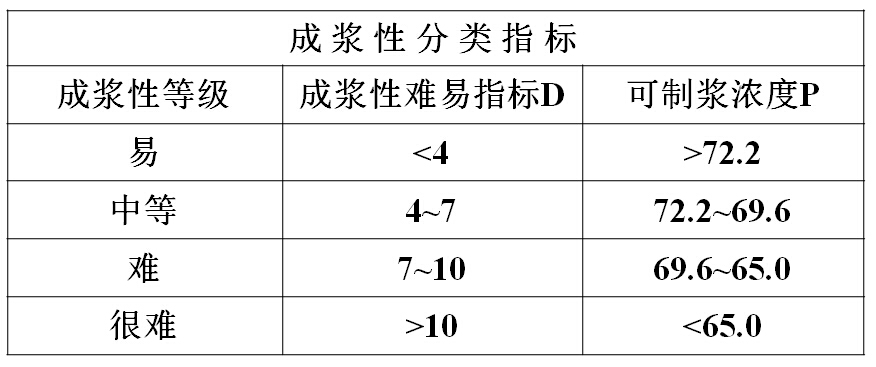
\includegraphics[scale=0.7]{30}
\caption{煤的成浆性评定表 }
\end{figure}
表中指标只供评价煤成浆性难易的相对比较而用,实际制浆浓度还取决于制浆的粒度分布与添加剂配方等因素。
$$D=7.5+0.5Mad-0.05HGI $$
$$C=77-1.2D(\%) $$
~~~~~~~~~~~~~~~~~~~~~~~~~~~式中:D——煤成浆性难易指标,\par
 ~~~~~~~~~~~~~~~~~~~~~~~~~~~ HGI——煤炭可磨性指数,\par
  ~~~~~~~~~~~~~~~~~~~~~~~~~~~~~~C——成浆浓度,\%;\par
 ~~~~~~~~~~~~~~~~~~~~~~~~~~~~ Mad——分析基水分,\%。
\subsection{改善煤成浆性的措施}
\begin{itemize}
\item 配煤成浆
 \item 压力处理
\item 热力处理
\item 新型添加剂的研究与应用。

\end{itemize}
\section{水煤浆制浆工艺}
水煤浆根据厂址划分,可分为用户型、矿区型和中央型三种。用户型水煤浆厂建在用户附近,使用外来煤,就地制浆,就地使用,使用管理方便,缺点是用户需新增一套水煤浆制备设施,并需培训专门人才;矿区型水煤浆厂建在选煤厂或矿区附近,原料供给方便可与选煤厂某些设施;中央型水煤浆厂建在矿区和用户以外的独立工业场地,生产的水煤浆供给若干用户,其投资最大。\par
    根据水煤浆厂处理能力的大小,又分成几种厂型:①小型厂:<10万t/a;②中型厂:10-50万t/a;③大型厂:50-100万t/a;④特大型厂:>100万t/a.
 \subsection{确定制浆工艺的依据}
制浆工艺即CWM制备工艺,水煤浆制备的关键技术有煤种选择、级配技术和添加剂技术。水煤浆主要技术参数见表
     \begin{figure}[!ht]
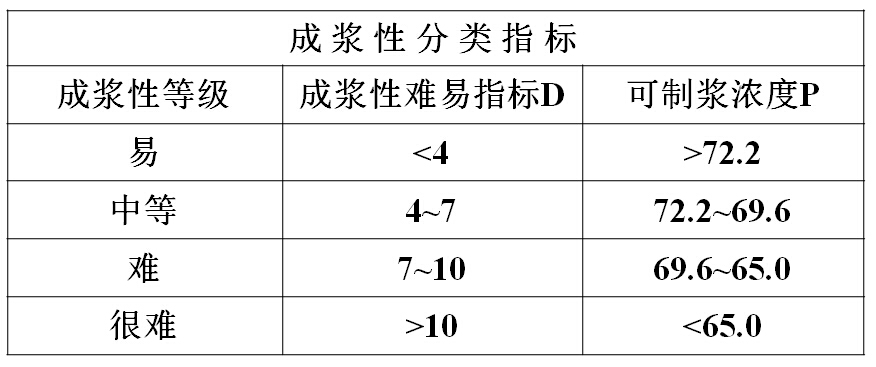
\includegraphics[scale=0.6]{30}
\caption{水煤浆主要技术参数}
\end{figure}
\subsubsection{原料煤特性}
原料煤是制浆的基础,从确定工艺的角度要掌握煤的可磨性、粒度组成、密度、成浆性等。
\subsubsection{级配技术}
级配技术为水煤浆产品中颗粒大小的组成情况,将原料煤磨成水煤浆产品,要求产品的粒度组成有较高的堆积效率,堆积孔隙最小,大颗粒间孔隙被小颗粒充填,以次减少空隙的水量,提高制将浓度,改善产品流动性。
\subsubsection{添加剂特性}
CWM添加剂,根据在CWM中所起作用不同分成分散剂、稳定剂、助剂等。\par
分散剂的主要作用是改变煤表面亲水性,降低煤水界面张力,使煤粒充分润湿和均匀分散在少量水中,改善CWM的流动性,降低CWM的粘度。\par
    稳定剂的作用是使煤粒在水中保持长期均匀分散,防止其中的粗粒在重力或振动力作用下发生沉淀。\par
    不同的煤种适应的添加剂不尽相同,在CWM制备中,不仅与所用添加剂的类型、数量有关,还与添加剂的添加方式和添加点有关。\par
 在确定CWM制备工艺时,应注意以下三点:\par
 1)选择满足用户要求的煤种,作为流体燃料CWM。对制备CWM的原料要求:灰分<10\%,硫分<1.0\%,Vdaf>30\%,ST>1300℃,成浆性要好,易于制成高浓度CWM.(根据D,判断成浆难易)。\par
    2)添加剂选择要遵循性能价格比最优原则,同时对煤种适应性要强,无毒无环境污染。\par
    3)在CWM级配上,CWM中煤粉的堆积效率要高。
\subsection{制浆方法的主要环节及功能}
 CWM制备工艺通常包括选煤(降灰、脱硫)、破碎、磨矿、加入添加剂、捏混、搅拌于剪切,以及为剔除最终产品中的超粒与杂物的滤浆等环节。
\subsection{制浆工艺 }

干法制浆工艺, 典型的干法制浆工艺流程如图所示:
     \begin{figure}[!ht]
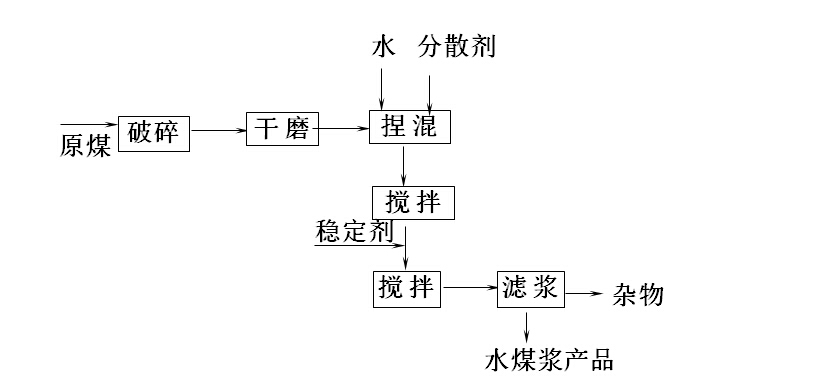
\includegraphics[scale=0.6]{32}
\caption{干法制浆工艺}
\end{figure}
\subsubsection{湿法制浆工艺}
湿法制浆工艺,从制浆原料上分,有末精煤制浆工艺和浮选精煤制浆工艺两种;从制浆浓度上分,有高浓度湿法制浆、中浓度湿法制浆和高、中浓度磨矿级配制浆工艺。
\section{水煤浆添加剂}
化学添加剂主要作用在于(1) 改变煤颗粒间的表面性质,提高煤炭表面的亲水性,降低煤水界面间的张力;(2) 促使煤粒表面能更容易被水润湿, 使煤颗粒均匀地分散在水中,防止颗粒团聚;(3)借助于添加剂调节煤浆的酸碱度、消除浆体中的气泡和有害成分等不利因素。 \par
    制浆时所用添加剂,按其功能不同,有分散剂、稳定剂、及其他一些辅助化学药剂,如消泡剂、PH调整剂、防霉剂、表面改性剂及促进剂等多种。在这些添加剂中,不可缺少的是分散剂与稳定剂。
    \subsection{分散剂的作用机理}
分散剂是一种可促进分散相(如水煤浆中的煤粒)在分散介质(如水煤浆中的水)中均匀分散的化学药剂。\par
       在水煤浆制备中分散剂的主要作用是降粘。分散剂的作用机理可从三个方面即润湿分散作用、静电斥力分散作用和空间位阻力与熵斥力分散作用得到解释。
       \subsubsection{润湿分散作用}
润湿是指固体表面上的气体被液体取代的过程,在讨论水煤浆问题时,润湿是指煤炭表面为水所润湿。\par
    水是一种极性物质,具有较高的表面张力,煤炭是非极性碳氢化合物,具有较低的表面能,被称为疏水性物质。但也存在容易为水所润湿的亲水部分,主体是芳烃,并通过烷烃链或原子彼此相连成为大分子结构。这些芳烃与烷烃属疏水性物质,杂原子或杂原子团属亲水性物质。杂原子主要是氧、氮和硫等,其中氧官能团有羟基(-OH)、羰基(=C=O)、羧基(-COOH)。羟基和羧基的亲水性最强,但羧基随煤化程度加深而减少,所以煤炭对水的亲疏程度与煤中芳烃及烷烃与羟基含量比有关。\par
    煤中的芳环数随煤化程度的加深而增加,所以,煤炭表面的润湿性也大体上是随煤化程度的加深而增强,各类煤炭表面接触角见表。此外,煤炭中的矿物质也属亲水性。

     \begin{figure}[!ht]
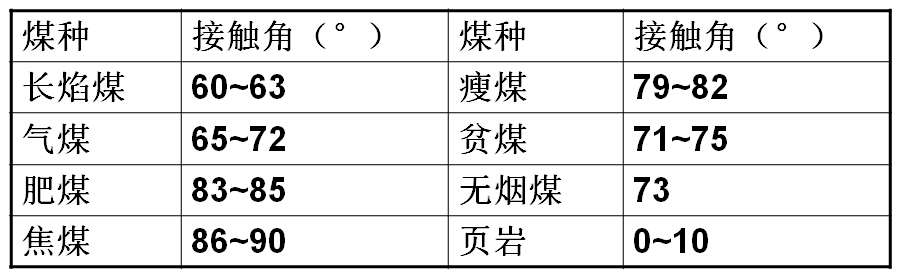
\includegraphics[scale=0.6]{33}
\caption{煤炭表面接触角}
\end{figure}
润湿过程可分为三种类型,即沾湿、浸湿和铺湿。\par
    沾湿是液体和固体表面接触,接触部分以固液界面取代了原有的固气界面和液气界面。\par
    浸湿是固体浸没在液体中,固气界面已为固液界面所取代,而液气界面未变。\par
    铺湿是在固液界面取代固气界面的同时,增加了液气界面。\par

通常将矿物的润湿性按接触角分成四类:\par
~~~~~~~~$\theta$=0° –强亲水性矿物;\par
~~~~~~~~0°<$\theta$<40°—弱亲水性矿物\par
~~~~~~~~40°<$\theta$<90°—疏水性矿物;\par
~~~~~~~~$\theta$>90°—强疏水性矿物\par
    我们在制备水煤浆时,既希望煤粒易于在水中分散,又希望能防止它再度发生聚结,并保持较稳定状态,应降低固液间的界面张力。

 \subsubsection{静电斥力分散作用}
         当颗粒相互接触时,如果没有其他力量的阻挡,聚结是不可避免的。微小粒子的热运动为颗粒间相互碰撞、接触创造了机会。\par
       颗粒间的吸引力来源于分子间的范德华作用力,它是由相互作用粒子内部偶极矩产生的,属电磁力。这种电磁力引起的吸力效果通常用吸引位能VA表示。\par
V$_A$/kT=A(d/s)\par
kT –动能,与颗粒直径立方成正比\par
V$_A$与颗粒直径四次方成正比。\par
颗粒间还存在静电的斥(吸)力。固体颗粒在水中由于表面物质电离,晶格取代或从溶液中吸附离子而表面带电。煤粒通常带负电。带电粒子总是要从周围溶液中吸引极性与它相反的离子,构成“双电层”。紧靠颗粒表面有一层溶液和反离子与颗粒实际上似为连成一体,可随颗粒一起运动。滑动面与溶液内部间的电位差ξ,称电动电位。\par
  两相同电荷的颗粒之间静电排斥电位V$_R$与kT之比为:V$_R$/KT=0.01 ξ$^2$ln(1+e$^{-s/δ}$ )
ξ对静电排斥力影响最大。 \par
    两个颗粒最终是吸引还是排斥,取决于范德华吸力与静电排斥力两者的综合效应V$_T$。在相距较远时,吸引力占优势,随着颗粒相互靠拢达到彼此的扩散层重合后,静电斥力开始起作用,且在某处达到最高值。由于吸引位能随距离减小增长比斥力位能快,越过能峰后,总位能迅速变成负值,进入净吸引区。由此可知在有足够的静电斥力作用下,如果颗粒所获外加能量不足以克服能峰就不会产生聚结。这就是依靠静电斥力的分散原理。\par
  一般外界因素不会对范德华引力产生影响,但颗粒间的静电斥力却受溶液环境影响很大。如溶液中离子浓度,特别是高价离子浓度增加,将压缩电动电位,使电动电位
ξ降低,双电层厚度δ变薄,使静电斥力迅速降低,甚至消失,使颗粒处于净吸力作用下,很快产生聚结,丧失稳定性。\par
\subsubsection{空间位阻与熵斥力分散作用}
所谓空间位阻分散作用,是指使煤粒表面吸附一层物质如添加剂、分子等,这样就在颗粒间增加了一层障碍,当颗粒相互接近时,可机械地阻挡聚结。制浆用分散剂都是一些表面活性剂,一端是由碳氢化合物构成的非极性的亲油基,另一端是亲水的极性基。非极性基疏水端易与煤炭表面结合,吸附在煤粒上,将另一端亲水基朝水。使煤粒的疏水表面转化为亲水表面,形成一层水化膜。使颗粒之间形成一种空间位阻。\par
    颗粒表面的吸附层具有一定的厚度,当两个带吸附层的颗粒相互接近,彼此重合时,由于吸附层中的高分子物质运动的自由度受到妨碍,吸附分子的熵减少,因为体系的熵总是自发地向增加方向发展,所以颗粒有再次分开的倾向,这就是熵斥力作用的后果。\par
    另外,添加剂在煤粒表面吸附膜的厚度能反映空间障碍的程度。
    \subsection{分散剂}  分散剂是最重要的化学添加剂,它一般是具有亲水基的物质,其作用主要是靠煤非极性表面天然疏水作用对分散剂疏水部分的吸附,使其亲水基朝外,以大大提高煤粒表面的润湿性,增厚稳定的水化膜,这种吸附作用也同时导致煤表面电性变化。但是,某种分散剂对某种煤制浆性能的好与坏,主要取决于煤表面对分散剂吸附能力以及这种分散剂亲水基的强弱。
分散剂属表面活性剂,大致可分离子型 ( 阳离子型、阴离子型 ) 和非离子型两大类。用于水煤浆的分散剂主要是阴离子和非离子型。阴离子型分散剂主要包括磺酸盐、羧酸盐及少量磷酸盐类;普遍应用的是荼黄酸盐、磺化腐植酸盐,木质素磺酸盐和烯烃磺酸盐等。这类阴离子型分散剂亲水基多为具有碱性的钠离子,其分散性能多不如非离子型,但由于原料来源较为广泛,生产工艺简单,价格低廉。非离子型分散剂,其特点是分子量大。这类分散剂分子的亲水端是聚氧乙烯链或再配以少许的磺酸基;亲固端是烷基、烷基苯或烷基苯羧酸等。此类分散剂的主要优点是亲水性好, 分子量和质量易调节、控制,不受水质及煤中可溶性物质的影响,但价格昂贵,一般用量在 0.5\% 以上。 \par
  对分散剂要求是:稳定性好,煤种适应性强,用量少,效能高,降粘效果明显;此外,价格也要经济。
\subsection{稳定剂} 水煤浆的稳定性是指煤浆在储存与运输期间保持性态均匀的特性。水煤浆的稳定剂应具有使煤浆中已分散的颗粒能与周围其他颗粒及水结合,成为一种较弱但又有一定强度的三维空间结构作用。稳定剂应在加入分散剂经捏混搅拌后,再另行加入。能起这种作用的稳定剂有无机盐、高分子有机化合物。如常见的聚丙烯酰胺絮凝剂,羧甲基纤维素以及一些微细胶体粒子(如有机膨润土)等。一般用量为煤量的几万分之几至几千分之几。
\subsection{其他辅助添加剂}
由于分散剂往往同时具有起泡作用,而煤浆中的气泡对浆体流动性有害,所以当分散剂带有较强的起泡性能时,需补加消泡剂。制浆时常用的消泡剂有醇类及磷酸酯类。\par
    为了取得较好的制浆效果,制浆时往往要调整煤浆的PH值,制浆时以弱碱性的溶液环境较好。\par
    助剂可改变煤炭表面性质、促进添加剂分子更好地在煤粒表面吸附。
    \section{水煤浆在贵州的应用}
 我省煤炭资源丰富,煤种齐全,又处在周边多是缺煤省的优越地理环境,生产适应市场的煤炭产品,既是我省经济发展的必然,也是适应国民经济发展的必须。\par
    水城矿区和盘江矿区是我省煤炭规模开发的两个矿区,已建成的煤炭生产能力13.3Mt/a,选煤能力10.6Mt/a.具备很好的启动水煤浆产业的基础条件.两矿区主要制浆原料煤煤质特征见表。

    \begin{figure}[!ht]
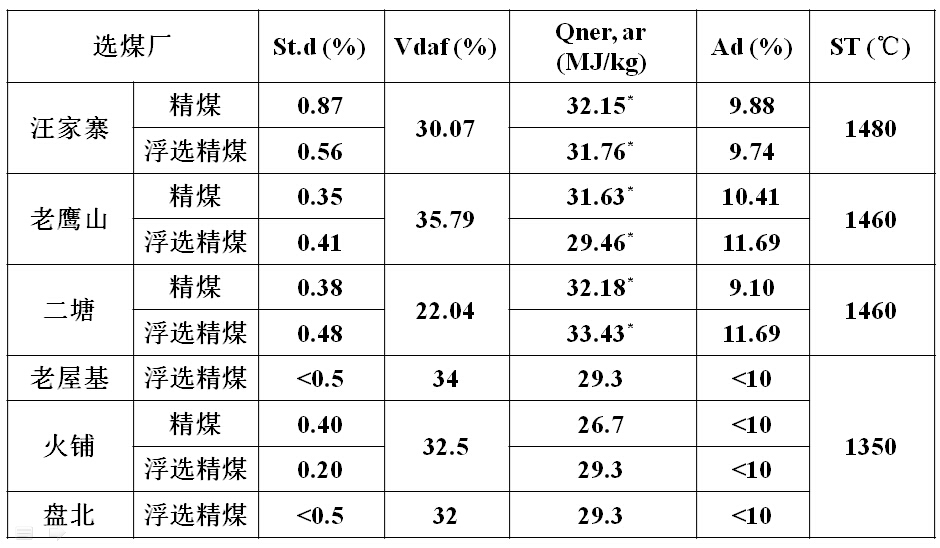
\includegraphics[scale=0.6]{34}
\caption{水城矿区和盘江矿区主要制浆原料煤煤质特征 }
\end{figure}

    \begin{figure}[!ht]
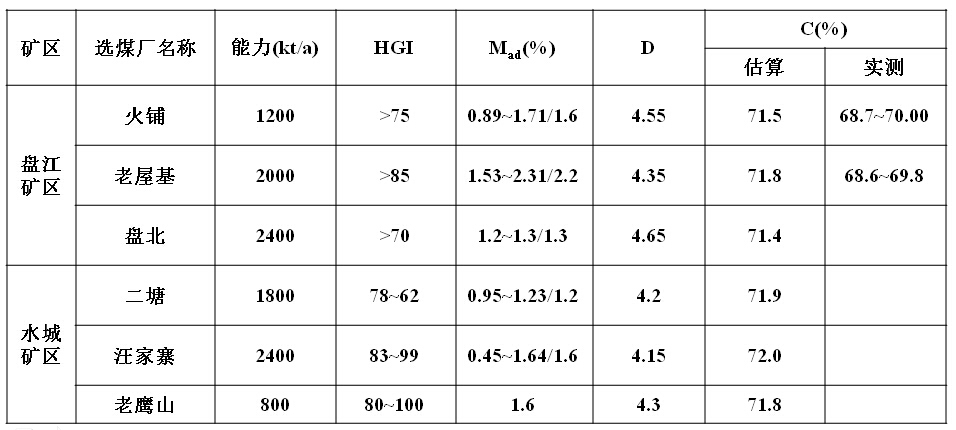
\includegraphics[scale=0.6]{35}
\caption{按照前述的成浆性数学模型~~ 水城矿区和盘江矿区煤成浆性预测}
\end{figure}
我省水煤浆技术产业化,按水煤浆的用途不同,近期宜从两个方面开展。
\subsection{精煤水煤浆}
    精煤水煤浆的主要用途是代油,我省燃油设备很少,据统计,贵阳市有50余台小规模的燃油锅炉,所以我省水煤浆的代油潜在市场在省外。\par
      广东省电力工业改烧水煤浆示范工程已经启动。
      茂名是 “盘浆”(盘江局生产水煤浆)南下进入广东省的第一站,铁路运输900km可直接达厂,于北浆(现使用的兖日水煤浆厂)海运到岸后再经车转运到厂比较,运输环节少,运输费省,另外盘江煤完全能制出比北浆更高品质(特别是发热量)的水煤浆,具有较强的市场竞争力。 \par
    海南省油电装机容量550MW,如全改烧水煤浆需1600~1800kt/a.这块市场的竞争对手是东方1-1天然气.初步估算,盘江水煤浆到厂价控制在420元/t内就有竞争力。\par
    水煤浆产业最大的特点是 “产浆”和 “用浆”几乎要一一对应,这是因为水煤浆作为一种新能源,传统的燃烧设备必须进行改造才能燃用,但一经改造设备又只能燃烧水煤浆,所以,在水煤浆用户不落实的情况下,建设浆厂必然存在很大的风险。\par
    用水煤浆代散煤锅炉主要是其节能、环保效益的体现。
    贵阳市的中、小型锅炉有1300余台,每年燃用原煤约1200kt,其中多为贵阳近郊的高硫散煤。这是造成贵阳市大气污染以二氧化硫和悬浮颗粒为主的煤烟型污染的主要污染源之一。用水煤浆替代散煤是解决这一难题的有效途径。若全改烧水煤浆,二氧化硫的排放量将降低为原来的20\%以上,烟尘污染将降低三分之二以上,燃煤垃圾将减少70-80\%,节能在20\%以上。但推广水煤浆代散煤需要解决以下问题。第一,锅炉必须改造,并且独立锅炉房都必须建设一套炉前储、送浆系统;第二,改烧水煤浆后燃料成本肯定增加,初步估算增加70\%左右,这比燃用城市煤气仍低约60\%。第三,同步建设水煤浆厂,若在贵阳市建设一座0.15Mt/a的水煤浆厂,投资在1800-2300万元之间,这可以避免水煤浆长途的运输。
    \subsection{煤泥水煤浆}
  我省水城和盘江两矿区上规模的选煤厂能力1060万t/a,按此计算,每年将产生近百万吨煤泥,目前利用这些煤泥的主要为低热值电厂,约占40\%。其它多作为排弃,甚至成为新的污染源。我国已有多处利用煤泥制浆就近供锅炉燃烧的成功先例。我省1994~1997年已在六枝局进行了煤泥制浆在35t沸腾炉掺烧的研究工作,项目由贵州省煤炭科学研究所和六枝矿物局承担,研究用地宗选煤厂洗选尾矿---煤泥,最大粒度600μm,平均粒度74.7μm,只需搅拌,而不用添加添加剂,即可制成水煤浆。水煤浆浓度55-58\%,稳定性一周,表观粘度在剪切率100S-1时为230mPa.s。水煤浆用泵直接送入给煤斗掺烧。该研究取得了成功,并通过了鉴定,取得了很好经济和环保效果。矿区利用煤泥,就近制成经济型煤泥水煤浆,供矿区厂矿锅炉燃烧,这样既可以利用这部分资源,改善矿区的环境,又可以降低成本,减少污染。
\chapter{煤的气化技术}
本章主要讲述煤的气化原理;气化用煤的特性;煤气化工艺分类,移动床、流化床、气流床和地下气化煤气化典型工艺以及煤气化技术的应用。 \par
    要求掌握煤气化的基本原理。
    熟悉气化用煤的特征;煤气化工艺分类。
    了解典型煤气化工艺;煤气化技术的应用。\par
    煤的直接燃烧带来的环境问题到目前为止仍不能得到有效地解决。而煤的气化技术可以说是未来煤的洁净利用技术的基础,被认为是最清洁的煤转化利用方式。\par
      煤的气化产物在电力生产、城市供暖、燃料电池、液体燃料和化工原料合成等方面都有极其广泛的应用,能够达到充分利用煤炭资源的目的,所以煤的气化技术理所当然成为未来洁净煤技术的核心。
      \section{概述}
      \subsection{煤气化的定义和实质}
    煤的气化过程是一个热化学过程,它以煤或煤焦为原料,以氧气(空气、富氧或纯氧)、蒸气或氢气为气化剂(又称气化介质),在高温的条件下,通过部分氧化反应将原料煤从固体燃料转化为气体燃料(即气化煤气,或简称煤气)的过程。煤气化是指煤在一定的温度和压力下,通过加入气化剂而被转化为煤气的过程。它包括煤的热解、气化和燃烧。\par
    煤炭气化时必须具备三个条件:气化炉、气化剂、供给热量。三者缺一不可。
    \subsubsection{气化与燃烧的区别}
从化学反应的角度,煤的气化和燃烧都属于氧化过程。当煤点燃时,它潜在化学能就会以热的形式释放出来,即空气中的氧气和煤中的碳、氢反应生成CO$_2$和H$_2$O,并释放热量;\par
  在氧气充足的情况下,煤将发生完全氧化反应,其所有的化学能都将转化成热能,这个过程就是燃烧。\par
 如果此时减少氧气量,那么煤将不能发生完全氧化反应,释放的热量也会减少,煤中剩余的潜在的化学能就会转移到生成的气体产物中,如H$_2$、CO、CH$_4$等。\par
  如果希望使气体产物中的化学能更大的话,从逻辑上讲就是继续减少供氧量。但实际上得有个限度,因为随着供氧量的减少,更多的煤将不能转化为气体而成为未反应碳,气化效率将大打折扣。所以控制供氧量至关重要。
 \subsubsection{气化与液化的区别}
 无论从工艺还是化学反应角度,两者都有很大不同。液化的目的是获取液体燃料或液体化学产品,其实质是通过将煤中大分子裂解成为小分子并同时调整煤中的C/H(减小)比以获得液体产物。包括加H$_2$直接液化和间接液化。
  \subsubsection{气化与干馏的区别}
干馏是煤在隔绝空气的条件下,在一定的温度范围内发生热解,生成固定焦炭、液体焦油和少量煤气的过程。\par
  而气化不仅是高温热解过程,同时还通过与气化剂的部分氧化过程将煤中碳转化为气体产物。\par
  从转化的角度看,干馏是将煤本身不到10\%的碳转化为可燃气体混合物,而气化则可将碳完全转化。\par
  对于气化和干馏还有一种理解:即将煤的气化分为完全气化和部分气化。其中部分气化就是指干馏技术。\par
  根据干馏温度的高低,又可以分高温干馏和低温干馏。高温干馏俗称高温炼焦,即冶金工业中炼焦;低温干馏又称温和气化,其工艺简单、条件温和,可同时获得煤气、焦油和半焦,因而是一项重要的洁净煤技术。
  \section{煤气化的基本原理}
\subsection{基本气化反应}
以典型的固定床气化炉为例,讨论煤在气化炉内经历的干燥、干馏、气化和燃烧几个过程。\par
气化炉中的燃料从上到下分为干燥层、干馏层、还原层、氧化层和灰渣层。
\subparagraph{干燥层}
湿煤加入气化炉后,依靠气体的显热,使煤中水分蒸发
\begin{center}
 湿煤——>干煤+H2O

\end{center}
\subparagraph{干馏层}
\begin{center}
干煤 ——>煤气(CO$_2$、CO、H$_2$、CH$_4$、H$_2$O、NH$_3$、H$_2$S)+焦油+焦
\end{center}
\subparagraph{还原层}
经干馏后得到的焦炭与气流中H2、CO2、H2O反应,生成可燃气体。
\begin{center}
C(焦)+H$_2$O  $\longrightarrow  $     CO+H$_2$+118.8 KJ/mol    \\
C(焦)+2H$_2$O $ \longrightarrow $     CO$_2$+2H$_2$+752.4 KJ/mol   \\
C(焦)+CO$_2$  $\longrightarrow  $     2CO +162.4 KJ/mol\\
C(焦)+2H$_2$  $\longrightarrow  $     CH$_4$-87.4 KJ/mol\\

\end{center}
\subparagraph{氧化层}
经气化后残留的焦与气化剂中的氧进行燃烧,放出热量以供气化反应所需。
\begin{center}
C(焦)+1/2O$_2$O  $\longrightarrow  $    2       CO~~-126.2 KJ/mol        \\
C(焦)+O$_2$O $ \longrightarrow $     2        CO$_2$~~-408.8 KJ/mol   \\


\end{center}
\subparagraph{灰渣层}
燃烧反应后残渣称为灰渣,进入灰渣层,气化剂在灰渣层与热灰渣进行热交换,使气化剂预热、灰渣冷却。\par
    在干燥层上部有一自由空间,干馏煤气与气化气混合,煤气中部分组成在此进行二次反应,决定出口煤气的组成。
\begin{center}
CO+H$_2$O $\longrightarrow  $     CO$_2$+H$_2$~~~-42.3 KJ/mol     \\
CO+3H$_2$ $\longrightarrow $     CH$_4$+H$_2$O~~~-206.2 KJ/mol    \\
CO$_2$+4H$_2$      $ \longrightarrow  $    CH$_4$+2H$_2$O~~~-162.9 KJ/mol


\end{center}

在气化炉中,煤气化分层过程实际上并不明显,层与层之间是交错的,尤其对其它型式床层气化炉(如流化床)就无分层现象。\par
为了使气化过程顺利进行,必须具备三个基本条件:
\begin{itemize}
\item 有足够数量的气化剂;
\item 有足够的热量;
\item 及时引出生成的煤气并排出灰渣。
\end{itemize}
\section{气化用煤的特性}
在选择煤气化工艺时,考虑气化用煤的特性及其影响极为重要,因为不同的气化工艺对原料煤质的要求不同。气化用煤的特性主要包括煤的反应性、粘结性、结渣性、热稳定性、机械强度、粒度组成以及水分、灰分和硫分等。
\subsection{煤的反应性}
是指在一定的外部条件下,与气化剂(氧气、水蒸气)相互作用并发生反应的能力。它直接影响煤在气化过程中的氧耗量、煤气组成、带出物与灰渣的含碳量、产气率及热效率等生产指标。不论何种气化工艺,反应性好有利于煤的气化。一般煤化程度越低,挥发分含量越高,干馏后焦炭的比表面积越大,其反应活性就越好;煤中的丝碳含量越高,反应活性就越强。
\subsection{煤的粘结性}
煤的粘结性是指煤被加热到一定温度时,受热分解而先变为塑性状态,然后煤粒之间受膨胀压力的作用再相互粘结在一起的程度。它会影响气体在料层内流动的通畅性与在料层截面上分布的均匀性。传统煤气化用煤采用弱粘结性的煤。
\subsection{煤的结渣性}
      煤的结渣性是指煤中矿物质在燃烧和气化过程中由于灰分的软化熔融而形成渣块的能力。容易结渣的煤不宜作为气化原料。一般来说,煤的灰熔点(ST)越低,越容易结渣,因此,固态排渣气化工艺通常要求ST≥1250ºC。
\subsection{煤的热稳定性}
      煤的热稳定性是指煤在燃烧和气化过程中对热的稳定程度,即煤块在高温状态下保持原来粒度的能力。对于使用块煤作原料的固定床气化工艺来说,煤的热稳定性差将会增加煤料层内气体流动的阻力和带出物量,降低气化效率。
\subsection{煤的机械强度}
煤的机械强度是指煤块的抗碎、耐磨及抗压等综合性物理和机械性能。它涉及煤在输送和气化过程中能否保持所要求的粒度和筛分组成,机械强度较低的煤不能直接作为固定床气化的原料
\subsection{煤的粒度分布}
不同气化工艺对所用原料煤的粒度要求不同。固定床气化要求使用13-100mm的块煤,且煤的粒度尽可能均匀;流化床气化要求使用0-8mm的粉煤,且按煤料中的最大颗粒确定气体在气化炉内的流速;气流床和熔浴床气化分别要求使用<0.1 nm 和< 6mm的煤粉和细粒煤,且根据煤料中的最大颗粒确定煤料在气化炉内的停留时间。
\subsection{煤中水分、灰分及硫分}
原料煤中水分对气化过程的稳定运行和热效率有直接影响,且水分越低,越有利于气化。固定床气化时,煤料中水分必须保证气化炉顶部出口煤气温度高于其露点温度;流化床和气流床气化时,为了使煤料在破碎、筛分、输送及加料时能保持自由流动,要求煤料的水分应<5\%特别是采用干法加料的气流床气化,要求煤料的水分<2 \%。
\subparagraph{灰分}
煤料中的灰分往往是影响气化过程正常进行的主要原因之一。煤中灰分既因其影响灰渣含碳而造成碳损失,又因其为惰性成分而造成气化效率降低和气化炉生产能力的浪费。特别当固定床气化时,煤中灰分高往往是造成气化炉内严重“结疤”的主要原因之一。
\subparagraph{硫分} 煤中硫包括黄铁矿硫、有机硫和硫酸盐硫。气化过程中煤中硫主要以H2S形式及少部分以CO$_2$和CS$_2$等形式转入煤气中。含硫气体是产品煤气的有害杂质,须在送用户之前净化脱除。
\section{煤气化工艺分类}  常见的分类方法如下
\subsection{按煤料与气化剂的接触方式,煤气化工艺可分为}
\subparagraph{固定床气化} 也称为移动床气化。因为在气化过程中,煤料与气化剂逆流接触,相对于气体的上升速度而言,煤料下降很慢,甚至可视为固定不动,因此称之为固定床气化;而实际上,煤料在气化过程中确是以很慢的速度向下移动的,故又称其为移动床气化。
\subparagraph{流化床气化} 它是以小颗粒煤为原料,并在气化炉内使其悬浮分散在垂直上升的气流中,煤粒类似于沸腾的液体而剧烈地运动,从而使得煤料层内几乎没有温度梯度和浓度梯度。
 \subparagraph{气流床气化}
这是一种并流气化,用气化剂将煤粉带人气化炉内,也可将煤粉先制成水煤浆,然后用泵打人气化炉内。煤料在高于其灰熔点的温度下被气化剂气化,灰渣以液态形式排出气化炉。
\subparagraph{熔浴床气化} 也称熔融床气化,它是将粉煤和气化剂以切线方向高速喷人温度较高且高度稳定的熔池内,且池内熔融物保持高速旋转。作为粉煤与气化剂的分散介质的熔融物可以是熔融的灰渣、熔盐或熔融的金属。
\subsection{按向气化过程的供热力式,煤气化工艺可分为}
\begin{itemize}
\item 含氧气体鼓风气化。
\item 固体热载体供热气化。
\item 电加热气化。
\item 利用核能加热气化。


\end{itemize}
\subsection{按气化剂种类不同,煤气化工艺可分为}
\begin{itemize}
\item  空气/蒸汽气化。即以空气和水蒸气作为气化剂。
\item 富氧空气/蒸汽气化。即以富氧空气和水蒸气作为气化剂。
\item 氧气/蒸汽气化。即以氧气和水蒸气作为气化剂。
\item 氢气气化。指气化剂中含有高浓度的氢气。

\end{itemize}
\subsection{按气化炉内操作压力的高低,煤气化工艺可分为}
1)常压气化是指煤气化反应基本上在常压条件下进行。\par
2)加压气化。是指煤气化反应在加压条件下进行,且按压力高低又细分为\par
3)中压气化:指气化压力在3.0MPa 以下进行。 \par
4)高压气化:指气化压力高达7.0-10.0MPa 。\par
\subsection{按气化过程的排灰方式,煤气化工艺可分为}
1)固态排渣气化;
2)液态排渣气化。
\subsection{按是否加人催化剂,煤气化工艺可分为}
1)催化气化;
2) 非催化气化
\subsection{按气化过程是否连续进行,煤气化工艺可分为}
l)连续气化;
2)间歇气化。
\subsection{为了与地下气化相区别,煤气化工艺可分为}
l)地面气化;
2)地下气化。
\section{典型煤气化工艺}
所谓典型煤气化工艺,主要指在我国已经长期广泛应用的工艺、近年来我国引进消化和自行开发并已得到应用的工艺以及我国目前尚未使用但却有较好发展前景的工艺。
\subsection{移动床煤气化工艺}
    移动床煤气化工艺是以块煤为原料。煤料与气化剂分别从气化炉的顶部和底部人炉,煤气和灰渣则分别从气化炉的顶部和底部出炉。煤料与气化剂在气化炉内逆流接触,煤气中的大部分显热用于煤料的干燥与干馏,而灰渣的大部分显热用于气化剂的预热。因此,这是一种比较理想的煤完全气化方式。
    \subsubsection{混合煤气发生炉气化工艺}
    该工艺是以空气与水蒸气的混合物作为气化剂,产生的煤气因N2含量较高而热值低,故称为混合煤气发生炉气化工艺。
\paragraph{混合煤气发生炉}
混合煤气发生炉的形式很多,通常可根据气化原料煤种、加料方式、排灰方式及操作方式等特征进行分类。介绍两种最典型的机械化常压混合煤气发生炉。\par
   1)具有凸型炉篦的混合煤气发生炉\par
    在具有凸型炉篦的混合煤气发生炉中,使用较普遍的有两种形式,即 3M21型和 3M13 型。\par
  2)威尔曼一格鲁夏混合煤气发生炉\par
    威尔曼一格鲁夏(又称 WG 型)混合煤气发生炉也有两种形式:一种无搅拌装置,用于气化无烟煤、焦炭等非粘结性煤料;另种带有搅拌装置,用于气化弱粘结性烟煤。\par
\paragraph{气化过程}
根据气化反应进行的情况,气化炉内可分为灰渣层、氧化层、第一还原层、第二还原层及炉内顶部空间5个部分。当气化烟煤或褐煤等含有较高挥发分和含水较高的原料时,则在第二还原层的上部,还存在一个干馏干燥层,在此主要是借助上升气体所带显热,脱除煤料中的挥发分和水分。
\paragraph{主要工艺条件及其影响}
在已选定原料、设备及工艺流程的情况下,为了获得最经济的气化指标,必须选择最佳的工艺条件,主要包括:气化温度、料层移动速度、料层高度、鼓风速度及饱和温度。
\paragraph{气化指标及其影响因素}
煤的气化是一个复杂的物理和化学过程,原料煤、气化剂以及不同的气化方法和操作条件都会影响到煤气化效果,通常衡量煤气化效果的指标包括:\par
气化强度:指气化炉单位面积每小时所能气化的原料煤质量,单位是t/(m2·h),它反映了气化过程的生产能力;\par
碳的转化率:表示原料煤中碳的转化程度,一般碳转化率越高,灰渣中未转化碳的量越少。\par
    煤气组成与热值:煤气质量的好坏是用煤气的组成和热值来表征的。煤气热值的高低则取决于煤气中的可燃组分。比如:混合发生炉中的可燃成分主要是CO和H$_2$。\par
    煤气产率:煤气产率是指气化单位质量的煤料所产生的煤气的体积数,分为湿煤气产率和干煤气产率,前者是指煤气中含有水蒸气,而后者指干煤气体积。煤气的产率与煤料的水分、灰分、挥发分及固定碳含量有关,也受碳转化率和碳损失率的影响。\par
  碳损失率:气化过程中的碳损失包括随煤气带出气化炉的碳损失和随灰渣排出气化炉的碳损失。碳损失的量取决于煤料的性质、鼓风速度、水蒸气的加入形式以及气化炉的结构。一般带出碳损失以干煤计,排出碳损失以纯碳计。\par
    气化效率:气化效率也称为冷煤气效率是指产生煤气的热值与煤气产率的乘积与所用煤料的发热量之比。\par
     当使用热煤气时,分子项中还应考虑煤气的显热,此时,称为热煤气效率。\par
 热效率:指煤气和副产品的热量以及回收利用的热量之和占供给气化过程总热量的百分数。可见,热效率表达了气化过程中热量有效利用的程度。
\subsubsection{水煤气发生炉气化工艺}
所谓水煤气是指水蒸气与炽热的碳反应而生成的煤气由于这种煤气燃烧时火焰呈蓝色,故又称为蓝(水)煤气。
\paragraph{水煤气发生炉}
 水煤气发生炉与混合煤气发生炉的结构较相近,其主要差别在于水煤气发生炉必须采用干法排灰,且为间歇式操作。另外,水煤气生产主要以无粘结性的焦炭和无烟煤为原料,因而水煤气发生炉内通常不设搅拌装置。目前,国内较多使用 U.G.I.型水煤气发生炉。
\paragraph{水煤气生产过程}
水煤气生产亦是以空气和水蒸气作为气化剂,但生产过程是间歇式的。即首先向气化炉内鼓空气,使空气中的氧与煤料中的部分碳发生燃烧反应而放出热量,并将绝大部分热量积蓄在煤料层内。当积蓄的热量使煤料层达到生产水煤气所需的高温时,停止鼓空气。然后向气化炉内通蒸汽,使水蒸气与炽热的碳反应生产水煤气。随着煤料层温度的下降,当水蒸气分解率低到定程度后,停止通蒸汽,再向气化炉内鼓空气,如此循环往复每个操作循环一般由 6 个阶段组成。
\paragraph{气化效率及其影响因素}
水煤气生产过程的气化效率包括吹风阶段的效率和制气阶段的效率,两者综合在一起,便为总过程的气化效率。\\
    1)吹风效率\par
    吹风(即鼓空气)阶段的目的是为了在煤料层内积蓄尽可能多的热量,为制气阶段能分解更多的水煤气创造条件;同时,该阶段又是非生产气阶段,要求占用的时间尽可能短。吹风效率是指积蓄于煤料层中的热量与该阶段消耗的煤料所具有的热量之比。影响吹风效率的因素有料层温度、吹人空气量、氧化层厚度及料层总高度等。\\
    2)制气效率与总过程气化效率\par
  制气阶段是间歇式生产水煤气的生产性阶段,其目的是获得数量多、质量好的水煤气,同时获得较高的水蒸气分解率。制气效率是指生产的水煤气所含的热量与制气阶段所消耗的煤料的热量和积蓄在煤料层中的热量之和的比值。\par
    而总过程气化效率则是指生产水煤气所含的热量与所用煤料总热量的比值。影响制气效率和总过程气化效率的因素有料层温度、煤料反应性及水蒸气用量与流量等。

\subsubsection{两段式发生炉气化工艺}
所谓两段式发生炉,就是在一般单段发生炉上增设一个干馏段,从而将煤的低温干馏和完全气化集中在一起连续进行。它既吸收了煤干馏时产生热值较高的干馏煤气的特点,又吸收了煤完全气化时产生数量较多的气化煤气的特点,因而可生产出热值较高、数量较多的产品煤气。同单段发生炉类似,根据操作方式的不同,两段式发生炉亦分为发生炉型两段炉与水煤气型两段炉。
\subsubsection{鲁奇加压气化工艺}
鲁奇加压气化工艺是最典型和成熟的移动床加压气化工艺。
\paragraph{加压气化过程分析}
    固定床加压气化过程与常压气化类似,所不同的是加压气化为甲烷化反应在气化炉内进行创造了条件。因此,固定床加压气化炉内的煤料自下而上可分为6层。即灰渣层、氧化层、还原层、甲烷层、干馏层及干燥层,其中的氧化层和还原层又被称为第一和第二反应层。
    \paragraph{气化压力的影响}
压力对气化过程的影响主要有以下几个方面:\\
1)气化压力对压缩气体动力消耗的影响\par
气化压力的提高,最显著的效果是节省动力,一体积的氧化对不同的煤种可产生5~10倍体积的煤气,因此,为了得到压力相近的煤气,压缩氧气的体积只占压缩煤气体积的10%-20 %。 \\
2)气化压力对煤气组成的影响\par
煤在加压下气化所产生的煤气中CH4和CO2含量增高,而CO和H2含量降低。净化后的煤气热值要随气化压力的提高而增高。\\
3)气化压力对氧耗量的影响\par
气化过程中所有生成甲烷的反应均是放热的,因而甲烷化反应不仅为吸热的气化反应提供了热量,而且也相应减少了参与吸热气化反应的碳量,从而减少了需碳和氧燃烧提供的热量。所以,加压气化减少了氧气的消耗。\\
4)气化压力对水蒸气耗量的影响\par
加压气化一方面因甲烷化反应所需的氢气而使蒸汽的需求量增加,另一方面又因加压不利于水蒸气气化反应的进行而使蒸汽分解率下降。因此,加压气化的水蒸气耗量明显高于常压气化。\\
5)气化压力对煤气产率的影响\par
加压气化虽然使得甲烷的生成量增加,但却使煤气的总体积减小,从而使得煤气产率下降,且因粗煤气中含有大量CO2而使净煤气产率下降的幅度比粗煤气更大。\\
6)气化压力对气化炉产气能力的影响\par
在加压条件下,气化过程的带出物和料层稳定性情况均有明显好转,因而,气化强度可以通过进一步提高鼓风速度而得
\subsection{流化床气化工艺}
    流化床气化工艺是以≤8mm的细粒煤为原料,同时作为流化介质的气化剂经底部气体分布板进入流化床气化炉并向上通过煤料床层。通过调节和控制气化剂的流速,可使煤料全部处于流化状态,并同时进行着气化反应和热量交换。产生的煤气夹带着大量固体细颗粒由炉顶离开气化炉,部分密度增大后的渣粒由底部排灰机构排出气化炉。
 \subsubsection{流化床的基本原理}
1)当气流速度较低时,固体颗粒保持静止,气体只在固体颗粒间的缝隙中穿过,床层高度基本保持不变,气体通过床层的压力降随气体流速的增大而增大。此时的床层称为固定床.\par
2)当气速增大时,固体颗粒开始松动,床层开始膨胀;如果气速继续增大,固体颗粒会形成最疏松的排列而失去永久接触的状态,如图中的C点。C点称为开始流化点,其对应的气速称为临界流化速度。\par
 3)随着气速的进一步增大,床层逐渐膨胀而增高。到达D点时固体颗粒已完全悬浮在上升的气流中,并呈现出相当不规则的运动状态,此时床层阻力趋于不变,已经进入完全流化状态。当气速继续增大时,床层高度随之增高,固体颗粒的运动更为剧烈,但仍停留在床层内而不被气流带出,且床层有一明显的上界面。此时的床层称为流化床。\par
4)当气速增大至超过图中的E点时,流化床的上界面消失,固体颗粒被上升气流带出,床层阻力随气速的增大而减小。此时的床层称为气流床。E点对应的气速称为流化床的气流极限速度,也称为固体颗粒的极限沉降速度。
    流化床的基本特性便可使用临界流化速度、床层压降、床层空隙率及气流极限速度等参数来表征。
 \subsubsection{流化床气化工艺的主要特点}
由于流化床内气固相间接触与返混良好,传质与传热效果理想,因此,流化床气化炉内的温度和浓度都均匀,从而使得煤的气化过程具有如下特点:\par
1)气化强度远高于固定床气化工艺。\par
2)气化温度低于固定床气化工艺,一般为800-1000 ℃左右。\par
3)煤料在800 ℃以上基本上不含焦油与酚等。\par
4)出炉煤气温度较高,显热损失较大。\par
5)碳的带出损失和排出损失均较大。
 \subsubsection{温克勒气化工艺}
温克勒气化工艺是最典型而成熟的常压流化床煤气化工艺,适合于气化褐煤、不粘煤、弱粘煤直至中等粘结性的烟煤。
\paragraph{温克勒气化炉}
它是一个内衬耐火材料的高大圆筒形容器,下部圆锥部分为流化床.上部圆筒形部分为气流床。煤料中的较大颗粒在下部的流化床中气化,而较小颗粒及气化过程中产生的细煤粒被气流夹带至上部的气流床时被引人的二次气化剂气化。二次气化剂量一般占气化剂总量的25\%-40\%。
\paragraph{温克勒气化工艺的优缺点}
与移动床气化工艺相比,温克勒气化工艺有下列优点:\par
1)单炉生产能力大;2)气化炉结构简单,造价低,操作与维护费用亦低;3)可气化细颗粒煤,而无需使用块煤;4)产生的煤气基本上不含焦油等,净化处理简单;5)生产负荷可在30\%-150\%范围内调节,且对气化效率基本上无影响。
温克勒气化工艺存在的问题主要有:\par
(1)由于气化温度较低,故只宜气化反应性好的煤料。(2)气化炉设备庞大,以体积计的气化强度仅为鲁奇炉的1/ 20,或 K一 T炉的1/ 3。(3)碳的排出损失与带出损失较多。
\subsubsection{高温温克勒气化工艺}
高温温克勒气化工艺(HTW)是在温克勒流化床气化工艺的基础上发展起来的,其改进之处主要在于:\par
1)将气化压力从常压提高到1.0Mpa,从而进一步提高了气化炉的产气能力,并使带出物量有所减少。\par
2)气化温度提高100℃左右,从而使碳转化率和气化强度均有所提高。\par
3)使带出物中的粗颗粒经分离回收后循环回气化炉气化,以提高碳转化率和减少碳损失。
\paragraph{高温温克勒气化炉}
高温温克勒气化炉的主体结构与常压温克勒气化炉并无太大差别,只是由于加压操作、温度提高、加石灰石床内脱硫及粗颗粒带出物循环回炉气化等特性而使其主要附属设备增多.
\paragraph{加压对流化床气化的影响}
所谓高温温克勒气化工艺,与常压温克勒气化工艺相比,实际上温度提高并不多,而压力的提高却对气化过程产生了很大的影响:\par
1)床层膨胀度随着气化压力的提高而急剧下降。\par
2)气化压力提高使床层结构得以改善,带出物量与带出颗粒的尺寸有所减小。\par
3)压力为 P 时的产气能力为常压流化床工艺的P$^{0.5}$倍。
\subsection{U-Gas气化炉}
U-Gas气化工艺借鉴了熔渣排灰的优点,采用灰团聚技术将流化床中的灰渣富集起来而排出,从而实现了流化床气化的选择性排灰。
\subsubsection{U-GaS 气化炉}
U一Gas气化炉的结构简图,它也是加压流化床气化炉。一部分气化剂从底部分布板进入气化炉以维持煤料床层的正常流化,其余气化剂则通过炉底倒锥形顶部的排灰管进人灰团聚区,使得此处温度高于周围的床层温度,且接近煤料的灰熔点。此时,含灰量高的粒子相互团聚、逐渐长大和增重,直到能克服从下逆流而上的气流的阻力时,便从床层中分离出来而落人炉底充水的灰斗内。\par
  随煤气从流化床顶部带出的细粉经过两级旋风分离器。第-级分离器出来的细粉返回流化床内气化;第二级分离器出来的细粉进人炉内的排灰区,经进一步气化和灰团聚后排人炉底灰斗。
 \subsubsection{U一Gas气化工艺的特点}
U一Gas气化工艺的主要特点是在流化床中灰渣与半焦的选择性分离,即煤气化后产生的灰经团聚成球形颗粒后从床层中分离出来。而灰粒的表面熔化及团聚成球则是一个较复杂的物理化学过程。
\subsection{KRW气化工艺 }
KRW气化工艺也是种灰团聚加压流化床气化技术.其基本特性与U 一 Gas 气化工艺相近,但二者间又有一些差别。
 \subsubsection{KRW气化炉}
KRW气化炉的结构简图。圆筒形炉体自上而下按其作用不同分为气固分离、气化、燃烧和团聚灰分离4段。煤料由高压输送气(空气或循环煤气)通过位于炉底中央的输送管连续不断地送人炉内。输送管顶端的喷嘴产生一股向上的射流而形成一个高温燃烧区。在高温燃烧区的上部,由于射流动能的逐渐减小与消失,煤粒便不再上升而转向四周,并沿气化炉内壁下降。就是靠这种环流颗粒的高速循环,把热量输送到整个床层。\par
在射流高温燃烧区内,含碳量较低的颗粒变得越来越软,相互碰撞后粘结变大而团聚成球。当团聚的灰球逐渐长大到不能再被流化时,便会落入炉底的倾斜段内,并被进人的循环煤气所冷却,然后落人下面的灰斗。
 \subsubsection{KRW与U一Gas两种气化工艺的比较}
KRW气化工艺与U 一Gas气化工艺的差别主要在于:\par
1)前者的气化压力高于后者。\par
2)前者以循环煤气作为流化介质,且用量较大,约为加人煤量的l~5 倍(重量比),而后者是以气化剂兼作流化介质。因此,前者的气氧比和气煤比均低于后者。\par
3)前者的煤料全部在高温燃烧区人炉,而后者的煤料则是从侧面人炉,并进人炉内还原区。 \par
4)前者团聚灰的分离和冷却采用循环煤气,余热由循环煤气带回气化炉得以利用,而后者团聚灰是在气化剂流中分离,用水淬冷,余热未利用。因此,前者的热效率高于后者。
\subsection{气流床煤气化工艺}
所谓气流床气化,是指将煤粉和气化剂通过特殊喷嘴喷入气化炉后,瞬间着火发生燃烧反应,燃烧区温度高达1500-2000℃。在气流夹带着煤粉上升的过程中,煤粉在几秒钟之内被气化。在反应区内,由于煤粒是悬浮在气流中并随之运动,煤粒间被气体隔开。因此,每个煤粒均单独经过膨胀、软化、烧尽后而形成熔渣,与其邻近的煤粒毫不相干。这样,煤料的粘结性、机械强度及热稳定性对气化过程几乎己不起作用。但气流床气化对熔渣的粘度一温度特性却有一定要求。
\subsubsection{气流床气化特性分析}
气流床气化的主要特征是煤料在气化炉内只停留几秒钟,气化温度高达1500~2000℃,且为液态排渣,因而要求:\par
  1)尽量用氧气和水蒸气作气化剂,以避免空气中的大量氮气人炉而使气化温度降低,从而有利于气化强度的提高和煤气质量的改善。\par
  2)选用反应性好、挥发分高、固定碳含量低的煤料有利于提高碳转化率和改善气化条件\par
  3)原料煤的粒度越细越好。
\subsubsection{气流床气化操作条件分析}

对气流床气化工艺而言,最重要的操作条件是气化温度、氧煤比及汽煤比。\par
   1)适当提高气化温度,不仅有利于加速气化反应的进行,而且有利于水蒸气气化反应平衡向生成CO和H2的方向移动,从而可提高产品煤气的质量。\par
   2)提高氧煤比是提高气化温度的主要手段,而氧耗又是主要的经济指标。综合考虑,在其它条件不变的情况下,氧煤比有一最佳值。\par
   3)在气化剂中加人适量的水蒸气不仅可以增加煤气中的氢含量,而且可以降低氧耗,同时还能调节和控制气化温度。\par
\subsubsection{K-T气化工艺}
    K一T气化工艺是最早工业化应用的气流床煤气化技术,它采用下部干粉进料、常压操作。 \par
    被磨得很细的煤粉 (90%以上小于0.1mm)同作为气化剂的氧气和水蒸气一起经设在炉头土的喷嘴从相对的方向喷人气化炉内,气化反应主要在炉头内完成。煤料中的大部分灰分在高温火焰区内被熔化,以熔渣形式沿气化炉内壁下流,至炉底后经水淬冷排出。这部分灰渣占总渣量的60%~70%,其余部分随煤气从炉顶带出。炉内煤气接近于该温度下水煤气的平衡组成。
 \paragraph{K 一T气化工艺的优缺点}
与移动床和流化床气化气化工艺相比,K-T气化工艺有以下优点:\par
   1)煤种适应性广,原则上可气化任何种类的煤料,最适宜气化反应性好、灰熔点较低的褐煤及年轻烟煤。\par
   2)水蒸气消耗量低。\par
   3)煤气中有效成分含量高,CO和H2含量合计高达90\%左右。 \par
   4)煤气中不含焦油和烃类,处理过程简单,不产生含酚废水。\par
K一T气化工艺的缺点在于:\par
   1)煤料制粉所需研磨设备较大,耗电较多。\par
   2)出炉煤气温度高,煤气除尘和余热回收负荷大,难度也高。\par
   3)宜用氧气作气化剂,且氧耗高,需昂贵的空分制氧装置。\par
   4)对用作炉衬的耐火材料要求较高。\par
\subsubsection{Texaco气化工艺}
Texaco气化工艺是采用水煤浆进料的加压气流床粉煤气化技术
\paragraph{Texaco气化炉}
Texaco气化炉的结构示意图。它为一个圆筒形压力容器,内壁衬有多层耐火材料。炉内上部为气化区,下部为煤气冷却区。水煤浆和氧气从炉顶喷嘴喷人气化炉后,瞬间着火发生燃烧和气化反应,炉温达1400 一1500 ℃,产生的灰渣呈熔融状态。粗煤气夹带着熔渣并流而下离开气化区进人煤气冷却区。根据煤气用途的不同,煤气冷却可采用水直接激冷式、废热锅炉间接冷却式或采用直冷与间冷相结合的方一式。
\paragraph{主要工艺条件}
影响Texaco气化炉操作工艺条件主要有水煤浆浓度、煤粉粒度、氧煤比、气化温度、气化压力以及煤料在气化区内的停留时间等。其中,水煤浆浓度对Texaco气化工艺是极为重要的,随着水煤浆浓度的提高,氧耗下降,煤气中的有效成分增加,气化效率提高。另外,为了维持正常生产,对水煤浆的稳定性和可泵送性也应给以重视。
\paragraph{Texaco气化工艺的特点}
与干粉进料的气流床气化工艺相比,Texaco气化工艺的优点是:\par
1)采用水煤浆进料,省去了干粉进料的加压煤锁等复杂机构,同时也避免了干粉进料时存在的不安全因素。\par
2)炉顶加煤,炉底液态排渣,有利于煤气与液态熔渣的分离。\par
3)气化炉结构简单,操作稳定。\par
\section{煤气化技术的应用 }
煤气在国民经济的各部门发挥着各种不同的作用,包括工业燃气、民用燃气、化工燃气、冶金还原气以及联合循环发电燃气等。\par
工业燃气:
       一般热值为1100-1350大卡热的煤气,采用常压固定床气化炉、流化床气化炉均可制得。主要用于钢铁、机械、卫生、建材、轻纺、食品等部门,用以加热各种炉、窑,或直接加热产品或半成品。\par
   民用煤气:一般热值在3000-3500大卡,要求CO小于10\%,除焦炉煤气外,用直接气化也可得到,采用鲁奇炉较为适用。\par
化工合成气化: 由于合成气化工和碳-化学技术的发展,使得以煤气化制取合成气,进而直接合成各种化学品的路线已成为现代煤化工的基础。主要包括合成氨、合成甲烷、合成甲醇、醋酐、二甲醚以及合成液体燃料等。\par
  冶金还原气:  煤气中的CO和H2具有很强的还原作用。在冶金工业中,利用还原气可直接将铁矿石还原成海棉铁;在有色金属工业中,镍、铜、钨、镁等金属氧化物也可用还原气来冶炼。\par
 联合循环发电燃气:
       整体煤气化联合循环发电(简称IGCC)是指煤在加压下气化,产生的煤气经净化后燃烧,高温烟气驱动燃气轮机发电,再利用烟气余热产生高压过热蒸汽驱动蒸汽轮机发电。用于IGCC的煤气,对热值要求不高,但对煤气净化度-如粉尘及硫化物含量的要求很高。 \par
       作煤炭气化燃料电池  :
       燃料电池是由H$_2$、天然气或煤气等燃料(化学能)通过电化学反应直接转化为电的化学发电技术。目前主要由磷酸盐型(PAFC)、熔融碳酸盐型(MCFC)、固体氧化物型(SOFC)等。 \par

 煤炭气化制氢  : 氢气广泛的用于电子、冶金、玻璃生产、化工合成、航空航天、煤炭直接液化及氢能电池等领域,目前世界上96\%的氢气来源于化石燃料转化。而煤炭气化制氢起着很重要的作用,一般是将煤炭转化成CO和H$_2$,然后通过变换反应将CO转换成H$_2$和H$_2$O,将富氢气体经过低温分离或变压吸附及膜分离技术,即可获得氢气。\par
煤炭液化的气源 :不论煤炭直接液化和间接氧化,都离不开煤炭气化。煤炭液化需要煤炭气化制氢,而可选的煤炭气化工艺同样包括固定床加压气化、加压流化床气化和加压气流床气化工艺。
 \chapter{煤的液化技术}
本章主要讲述煤的直接液化技术和煤的间接液化技术;
要求熟悉煤的直接液化和煤的间接液化概念;
了解直接液化和煤的间接液化工艺。\par
煤的液化是把“脏”的煤转化成既可高效洁净利用,又便于运输的液体燃料或化工原料的技术,即用煤作原料以制取液体烃类为主要产品的技术。煤液化分为“煤的直接液化”和“煤的间接液化”两大类。
\section{煤的直接液化}
\subsection{概述}
煤的直接液化是煤在适当的温度和压力下,催化加氢裂化(热解、溶剂萃取、非催化液化等)成液体烃类,生成少量气体烃,脱除煤中氮、氧和硫等杂原子的深度转化过程。典型的工艺主要包括原料煤的破碎与干燥、煤浆制备、加氢液化、固液分离、气体净化、液体产物分馏和精制以及液化残渣气化制取氢气等部分。直接液化的主要产品是优质汽油、喷气燃料油、柴油和芳烃以及炭素化工原料,并付产燃料气、液化石油气、硫磺和氨等。工艺热效率高达70\%。
\subsubsection{直接液化过程}
    煤炭直接加氢液化一般是在较高温度(>400℃),高压(>10MPa),氢气(或CO+H$_2$,CO+H$_2$O)、催化剂和溶剂作用下,将煤进行裂解加氢,直接液化为液体油的加工过程。\par
    煤与石油主要都是由C、H、O等元素组成,不同的是:煤的氢含量和H/C原子比比石油低,氧含量比石油高;煤分子量大,一般>5000,而石油约为200,汽油约为110;煤的化学结构复杂,煤还含有相当数量的以细分散组分的形式存在的无机矿物质和吸附水,煤也含有数量不定的杂原子(氧、氮、硫)、碱金属和微量元素。\par
加氢液化的实质是用高温切断化学结构中的C-C键,在键断裂处用氢来饱和,从而使分子量减小和H/C比提高。反应温度要控制合适,温度太低,不能打碎煤分子结构或打碎的太少,油产率低。一般液化工艺的温度为400-470℃。
\subsubsection{直接液化的原料煤}
煤的液化性能主要取决于煤的分子结构、组成和岩相组分含量,并与煤灰成分有关。适宜液化的煤一般是:\par
1)年轻烟煤和年老褐煤;\par
2)挥发分大于37%,灰分小于10\%;煤的灰分组成也对液化过程有影响,灰中的Fe、Co、Mo等元素有利于液化,对液化起催化作用;而灰中的Si、Ca、Mg等元素则不利于液化,它们易产生结垢,影响传热和不利于正常操作,也易使管道系统堵塞、磨损,降低设备的使用寿命。\par
3)氢含量大于5%,炭含量82-85\%,H/C比越高越好,同时希望氧含量越低越好;
\subsubsection{直接液化的溶剂}
在煤液化过程中,溶剂起着溶解煤、溶解气相氢向煤或催化剂表面扩散、供氢或传递氢、防止煤热解的自由基碎片缩聚等作用。根据相似者相溶的原理,结构与煤分子近似的多环芳烃,对煤有较大的溶解能力。煤液化的起始溶剂可以选用高温煤焦油中的蒽油馏分,也可采用石油减压蒸馏的渣油。
\subsubsection{直接液化的催化剂}
煤直接液化工艺使用的催化剂一般选用铁系催化剂或镍钼钴类催化剂,镍钼钴类催化剂活性高,用量少,因价格高,须反复使用。铁系催化剂,活性低,用量较多,但来源广且便宜,可不用再生。氧化铁和硫或硫化钠组成的铁硫系催化剂,也具有较高的活性。
\section{煤的间接液化}
\subsection{概述}
煤的间接液化是以煤基合成气(CO+H$_2$)为原料,在一定的温度和压力下,定向地催化合成烃类燃料油和化工原料的工艺,包括煤炭气化制取合成气、气体净化与变换、催化合成烃类产品以及产品分离和改质加工等过程。典型的工艺是F-T合成法,又称CO加氢法。\par
CO和H2在催化剂作用下的主要反应有:\par
\begin{tabular}{crl}

合成烷烃:& nCO+(2n+1)H$_2$  $\longrightarrow$& CnH$_{2n}$+(2+n)H$_2$O \\

 & 2nCO+(n+1)H$_2$  $\longrightarrow$ & CnH$_{2n}$+(2+n)CO$_2$ \\

合成烯烃:& nCO+2nH$_2$ $\longrightarrow$ & CnH$_{2n}$+nH$_2$O \\

 & 2nCO+nH$_2$          $\longrightarrow$ & CnH$_{2n}$+nCO \\

\end{tabular}
此外还有合成醇类等含氧化合物的反应。\par
对于F-T合成,主要是合成烷烃的反应以及少量合成烯烃的反应,所用的催化剂有Co剂、Ni剂和Fe剂等。因Fe剂便宜、选择性和操作适应性较好,可合成辛烷值较高的汽油,故多在工业上使用。铁剂又分为沉淀铁剂和熔铁剂,前者用于低温(200-280℃)和固定床反应,后者可用于较高温度(280-340℃)和气流床反应。压力升高有利于合成反应,但压力影响催化剂的活性和寿命,铁剂一般用在中压(0.7-2.5MPa)。合成气中H$_2$/CO比值高,有利于生成饱和烃和轻产物,一般还要控制合成气含硫量以防止催化剂中毒。
煤制备其他液体燃料
\subsection{煤制备其他液体燃料}
\subsubsection{煤制甲醇的典型工艺}
20世纪初,人们发现CO和H2体系在铁系催化剂作用下合成的液体油中,有甲醇存在。其后开发出了铬锌(均为氧化物)为催化剂的高压合成甲醇技术,其反应条件为:压力:25-35MPa,温度:320-400℃
其基本原理为:
$$CO+H_2 \longrightarrow CH_3OH~-Q $$
$$CO_2+3H_2 \longrightarrow CH_3OH+H_2O~-Q $$
\subsubsection{甲醇转化成汽油(MTG)}
其原理过程为:CH$_3$OH$\longrightarrow$ CH$_3$OCH$_3$ $\longrightarrow$ 轻烯烃 $\longrightarrow$ 重烯烃
在催化剂选择作用下,烯烃可以重整得到脂肪烃、环烷烃和芳香烃,但一般所得碳原子数不会超过10。
\subsubsection{煤制二甲醚的典型工艺}
二甲醚DME,又称木醚,氧二甲。工业上主要是通过甲醇气相催化脱水工艺和合成气直接合成二甲醚工艺生产二甲醚。
\subsection{我国煤间接液化技术}
由中科院山西煤化所承担的“十五”863能源领域课题“煤间接液化技术”通过验收。该课题在催化剂和浆态床反应器中试技术方面取得了重要突破,并已取得专利20余项。 \par
该课题所建成的750吨级中试装置已实现了1500小时稳定运行,并生产出一批合成粗油品大样,这些样品经处理,柴油产品质量达到了欧4标准,十六烷值达75,技术指标达到国际先进水平。该技术的突破,为我国今后煤炭间接液化技术的工业应用奠定了良好基础,对我国实现煤炭清洁高效利用具有重要意义。\par
兖矿百万吨级煤炼油工业化示范装置将于2007年启动,在“十一五”规划中将实现200万吨的煤制油产能。而神华集团“煤变油”项目一期工程生产线将年生产各种油品320万吨。二期工程生产线将于2010年投产,建成后将年生产各种油品280万吨。\par
 投资288亿元、年产800万吨石油的宁夏煤炭间接液化项目,目前已进入科研论证阶段。宁夏煤业集团“煤变油”项目计划于2008年开工建设,2011年建成投产。
然而,由于项目前期投入巨大、动辄需要数百亿的资金,加之转换过程中产生巨大环境成本的风险问题等,因此,对于煤制油项目也存在诸多争议。持反对观点的专家认为,缓解能源紧张并不意味着必须发展煤制油,虽然中国煤炭总体储量不小,但人均煤炭占有量只有世界平均值的60\%左右。以一种稀缺资源去替代另一种稀缺资源,迟早是要付出代价的。

%\newpage
%~~~
%\thispagestyle{empty}
%\newpage
%~~~
%\thispagestyle{empty}
%\ThisCenterWallPaper{1}{56}
\end{document}
